\documentclass[11pt]{article}

% ============================ PREAMBLE ============================
\usepackage[utf8]{inputenc}
\usepackage[T1]{fontenc}
\usepackage{lmodern}
\usepackage{amsmath,amsthm,amssymb}
\usepackage{booktabs}
\usepackage[margin=1in]{geometry}
\usepackage{graphicx}
\graphicspath{{figures/}}
\usepackage{enumitem}
\usepackage{xcolor}
\usepackage{microtype}
\usepackage[numbers]{natbib}
\emergencystretch=3em        % last-resort stretch to avoid overfull \hbox page overflow
\tolerance=2000
\setlength{\parskip}{2pt}
\usepackage[colorlinks=true,linkcolor=blue!55!black,citecolor=green!45!black,urlcolor=blue!60!black]{hyperref}

% ---- math shortcuts ----
\newcommand{\R}{\mathbb{R}}
\newcommand{\E}{\mathbb{E}}
\newcommand{\N}{\mathbb{N}}
\DeclareMathOperator{\Var}{Var}
\DeclareMathOperator{\Cov}{Cov}
\DeclareMathOperator*{\argmin}{arg\,min}
\newcommand{\clip}{\operatorname{clip}}

% ---- theorem environments ----
\theoremstyle{plain}
\newtheorem{theorem}{Theorem}
\newtheorem{proposition}[theorem]{Proposition}
\newtheorem{lemma}[theorem]{Lemma}
\newtheorem{corollary}[theorem]{Corollary}
\theoremstyle{definition}
\newtheorem{definition}[theorem]{Definition}
\newtheorem{assumption}{Assumption}
\theoremstyle{remark}
\newtheorem{remark}[theorem]{Remark}

\title{An Optimization View of DP LLM Fine-tuning:\\
When Does Bias Correction Help, and Can the Optimizer Be Improved?}

\author{Zixuan Wang}

\date{Optimization Methods for Artificial Intelligence Course Project \\[2pt] \small (compiled \today)}

\begin{document}
\maketitle

% =====================================================================
%  ABSTRACT
% =====================================================================
\begin{abstract}
Differentially private (DP) fine-tuning of large language models runs on DP-SGD/DP-Adam,
and the field's reflex when DP noise hurts utility is to \emph{fix the adaptive
preconditioner}. The reference for this report, DP-AdamBC \citep{tang2024dpadambc}, does this
analytically: it subtracts the closed-form DP-noise variance bias $\Phi=(\sigma_{\mathrm{DP}}C/B)^2$
from Adam's second moment $\hat v$. We take an \emph{optimization view} and ask when that
correction actually helps in LLM DP-LoRA fine-tuning, and whether any principled optimizer
change can beat a well-tuned, privacy-amplified DP-Adam at the same $(\varepsilon,\delta)$.
Our organizing quantity is the \emph{noise share} $\rho:=\Phi/\hat v=\Phi/(v_{\mathrm{true}}+\Phi)\in[0,1]$,
a one-line, a-priori diagnostic for whether bias correction can do anything. We prove and measure
that in the standard recipe $\rho$ \textbf{saturates at $\approx 1$}: the second moment is an inert
noise floor carrying no per-coordinate signal, and learning instead rides the \emph{first} moment
$\hat m$ (a gradient prefix-sum that averages the zero-mean DP noise toward a below-floor signal).
Consequently bias correction \textbf{collapses to momentum-SGD} at $\rho\!\approx\!1$ and is only an
\textbf{effective-learning-rate knob} at $\rho\!<\!1$; four controls (a floor sweep, a floor-only
control, a learning-rate control, and a Muon-geometry probe), two models, and three seeds show it
never robustly beats a tuned DP-Adam, whose learning-rate plateau ($\approx 56.7$ proxy BLEU)
matches the best DP-AdamBC ($56.73$). We then \emph{attempt a positive method}, DP-CorrMom: anti-correlated
DP noise $w_t=z_t-\lambda z_{t-1}$ injected on the first-moment / prefix-sum path
(a DP-FTRL / matrix-factorization mechanism), and find a \textbf{unified negative}---across
Adam-momentum, $\beta_1{=}0$, and the matched plain-SGD workload, $\lambda{>}0$ never beats
$\lambda{=}0$, and a privacy-\emph{amplified} DP-Adam wins at less budget. We explain this with a
\emph{signal-ceiling} theorem: at $\rho\!\approx\!1$ the model is \textbf{signal-limited, not
variance-limited}, so once basic averaging has extracted the recoverable signal, further noise
reduction cannot help---which is precisely why correlated-noise mechanisms that provably help
\emph{from-scratch} SGD do not transfer to LLM DP-LoRA fine-tuning. Beyond the reference, we
contribute (i)~the $\rho$ diagnostic, (ii)~the $\hat m/\hat v$ mechanism, (iii)~a four-control
attribution of DP-AdamBC, (iv)~a verified privacy-sensitivity correction
$\kappa=\sqrt{(1-\lambda^{2T})/(1-\lambda^2)}$ for $w_t=z_t-\lambda z_{t-1}$ (the naive $\sqrt{1+\lambda^2}$
\emph{breaks} privacy), and (v)~the signal-ceiling theorem for first-moment denoising---none of
which appear in DP-AdamBC. \emph{Honesty markers:} the E2E utility is a teacher-forced proxy BLEU,
and the positive-method sweeps are single-seed (consistent across five variants).
\end{abstract}

% =====================================================================
%  INTRODUCTION & MOTIVATION
% =====================================================================
\section{Introduction and Motivation}
\label{sec:intro}

Differential privacy \citep{abadi2016deepdp,mironov2017renyi} has become the default formal
guarantee for fine-tuning language models on sensitive text. The workhorse is DP-SGD: clip each
per-sample gradient to $\ell_2$-norm $C$, add isotropic Gaussian noise of scale
$\sigma_{\mathrm{DP}}C$, and average over a batch of size $B$. The Gaussian mechanism therefore
injects, \emph{per coordinate}, a variance
\begin{equation}
\label{eq:phi-intro}
\Phi \;:=\; \Big(\frac{\sigma_{\mathrm{DP}}\,C}{B}\Big)^2,
\end{equation}
that is \emph{independent of the parameters} and does not vanish at the optimum---it is the
irreducible price of privacy. When DP-Adam is used instead of DP-SGD, this same $\Phi$ silently
contaminates Adam's second-moment estimate $\hat v$, biasing the adaptive preconditioner.

\subsection*{Two-fold motivation}

This report is driven by two questions that the literature poses but, for LLM fine-tuning, leaves
open.

\paragraph{Motivation A --- Does the field's go-to fix actually hold here?}
The dominant response to ``DP noise corrupts the optimizer'' is to repair the adaptive
preconditioner. The reference paper, \textbf{DP-AdamBC} \citep{tang2024dpadambc}, gives the cleanest
instance: because $\E[\hat v]=v_{\mathrm{true}}+\Phi$, it simply subtracts the analytic bias,
$\hat v^{\mathrm{BC}}=\max(\hat v-\Phi,\xi)$, restoring Adam's intended geometry. This is principled
and reports gains. But \emph{when}, in the operating regime of LLM DP-LoRA fine-tuning, does
removing $\Phi$ translate into utility---and is the gain anything other than a step-size effect that
a practitioner could obtain by simply re-tuning the learning rate? An optimization-view answer
requires (i) an a-priori test for whether the correction is even active and (ii) controls that
separate genuine per-coordinate de-biasing from a scalar learning-rate change.

\paragraph{Motivation B --- If the second moment is a dead lever, can a \emph{different}
optimizer change win?}
If bias correction turns out inert, the natural next move is to ask whether \emph{any} principled
change to the private optimizer---changing what we denoise, the update geometry, or the
\emph{temporal structure} of the injected noise---can beat a well-tuned, privacy-amplified DP-Adam
at the same $(\varepsilon,\delta)$. This connects to a deep and currently fashionable line of work:
correlated-noise / matrix-factorization mechanisms (DP-FTRL and successors) that provably reduce the
error accumulated along the gradient \emph{prefix-sum}. The question is whether that provable
advantage, established largely for \emph{from-scratch} training, transfers to gentle LLM fine-tuning.

\subsection*{How the literature attacks DP-optimizer utility (four lines)}

We situate both motivations against the four families of optimizer-side remedies in the DP literature.

\begin{enumerate}[leftmargin=2em,itemsep=2pt,topsep=2pt]
\item \textbf{Fix the second moment.} Subtract the analytic noise bias $\Phi$ from $\hat v$ so the
adaptive preconditioner is no longer poisoned by DP noise---\emph{DP-AdamBC}
\citep{tang2024dpadambc}, our reference. This is the line Motivation~A interrogates.

\item \textbf{Reduce the noised dimension.} Privatize gradients in a lower-dimensional subspace
(random projection or learned low-rank), so less Gaussian noise is needed for the same
$\varepsilon$---e.g.\ \emph{DP-GRAPE} \citep{dpgrape2025} and gradient-embedding perturbation. The
floor's linear dependence on dimension (our Corollary in \S\ref{sec:theory}) is exactly what this
exploits; LoRA is itself a coarse instance.

\item \textbf{Re-allocate the clip/noise budget.} Spend the clipping and noise budget unevenly
across parameter groups so high-signal layers are noised less---group-wise clipping
\citep{he2023groupclip}.

\item \textbf{Correlate the injected noise across time} so it cancels along the gradient prefix-sum:
\emph{DP-FTRL} \citep{kairouz2021dpftrl}, matrix factorization \citep{denisov2022mf},
banded matrix factorization \emph{BANDMF} \citep{choquettechoo2023bandmf}, the proof that
``correlated noise provably beats independent noise'' \citep{choquettechoo2024correlated}, the
single-scalar \emph{DP-$\lambda$CGD} \citep{dplcgd2026}, and buffered linear toeplitz \emph{BLT}
mechanisms \citep{blt2024}. This is the line Motivation~B tests, and the source of our positive-method
attempt.
\end{enumerate}

\subsection*{What we find: numbered prior findings vs.\ our results}

Against these four lines, our optimization-view study produces five results. We number them so the
empirical sections (\S\ref{sec:numerical}) can refer back to each; every number below is grounded in the
project's recorded experiments.

\begin{description}[leftmargin=1.4em,itemsep=3pt,topsep=2pt]
\item[\textnormal{(R1)} The noise share $\rho$ saturates at $\approx 1$.]
Measuring $\rho=\Phi/\hat v$ live during training, we find $\rho=1.00$--$1.07$ across
RoBERTa-large/MNLI (all $\varepsilon\in\{1,3,8\}$, all $B\in[16,2048]$) and Qwen2.5-1.5B/E2E
($B\!\le\!512$); $\rho$ drops below $1$ only when the batch is pushed to $B{=}4096$ at
$\varepsilon{=}8$ ($\rho{=}0.955$). \textbf{The DP-LoRA gradient signal lies below the noise
floor}, so the bias-correction sweet spot $\rho\!\approx\!\tfrac12$ is structurally out of reach.

\item[\textnormal{(R2)} Learning rides the first moment, not the second.]
Models still learn at $\rho\!\approx\!1$ (proxy BLEU $\approx\!56$ vs.\ a DP-SGD floor $\approx\!21$)
because Adam's update is $\hat m/\sqrt{\hat v}$: the \emph{first} moment $\hat m$ (a prefix-sum)
averages the zero-mean DP noise toward the below-floor signal over many steps, while $\hat v$ is a
near-constant noise level---\textbf{adaptivity is effectively switched off}. This resolves the
apparent paradox ``$\hat v$ is all noise yet the model learns.''

\item[\textnormal{(R3)} Against line~1: bias correction collapses to momentum-SGD ($\rho\!\approx\!1$).]
With $\hat v-\Phi\!\approx\!0$, every DP-AdamBC floor is fully clamped, so the update is
$\hat m/\sqrt{\xi}$---momentum-SGD with a \emph{fixed} step scale. Utility tracks the floor (a
learning-rate effect, three seeds), DP-AdamBC at a binding floor is statistically indistinguishable
from a floor-only control with \emph{no} $\Phi$-subtraction, and a Muon-style geometry probe
(line~2's discard-the-second-moment cousin) recovers no signal ($+8\times 10^{-5}$ cosine). The
saturation is fundamental to the noise level, not a preconditioner artifact.

\item[\textnormal{(R4)} Where it is active, bias correction is only an effective learning rate.]
At $\rho{=}0.955$ (large batch) DP-AdamBC genuinely de-biases ($\approx\!3.8\times$ larger step) and
leads at a short budget (step-40 $+1.2$ BLEU), \emph{but DP-Adam catches up and passes it by
convergence}. A learning-rate control settles it: tuned DP-Adam traces a clean inverted-U with a
plateau $\approx 56.7$ over $\mathrm{lr}\in[2,5]\times10^{-3}$ that matches the best DP-AdamBC
($56.73$). An earlier step-40 ``$+1.57$ win'' was correctly flagged as a convergence-speed transient
and overturned---\textbf{not overclaimed}.

\item[\textnormal{(R5)} Against line~4: the positive-method attempt is a unified negative.]
Motivated by R2 (learning rides the prefix-sum), we built \emph{DP-CorrMom}, anti-correlated noise
$w_t=z_t-\lambda z_{t-1}$ on the first-moment path, with verified privacy
($\kappa=\sqrt{(1-\lambda^{2T})/(1-\lambda^2)}$; $\lambda{=}0$ reproduces DP-SGD-momentum bit-for-bit).
Across Adam-momentum, $\beta_1{=}0$, and the \emph{matched} plain-SGD prefix-sum workload (DP-CorrSGD),
$\lambda{>}0$ never beats $\lambda{=}0$, and a privacy-\emph{amplified} DP-Adam beats all of them at
less budget. We explain this with a \textbf{signal-ceiling}: at $\rho\!\approx\!1$ the model is
signal-limited, so further noise reduction is wasted---\textbf{which is exactly why DP matrix
factorization, proven to help from-scratch SGD, does not transfer to LLM DP-LoRA fine-tuning.}
\end{description}

\subsection*{Contributions beyond the reference}

DP-AdamBC contributes the analytic $\Phi$-subtraction and demonstrates gains in its tested settings.
Relative to it, this report contributes, and clearly highlights for the bonus, five new results
(\S\ref{sec:new}): (1)~the $\rho=\Phi/\hat v$ \emph{noise-share diagnostic}; (2)~the $\hat m/\hat v$
\emph{mechanism}; (3)~the \emph{four-control attribution} showing DP-AdamBC $=$ effective LR /
momentum-SGD; (4)~the \emph{verified $\kappa$ sensitivity} for $w_t=z_t-\lambda z_{t-1}$, correcting
the wrong $\sqrt{1+\lambda^2}$ that under-noises and breaks privacy; and (5)~the \emph{signal-ceiling
theorem} for first-moment denoising. The report is organized as: background and setup
(\S\ref{sec:setup}), the mathematical theory with proofs (\S\ref{sec:theory}), the numerical
simulation in a question-driven voice (\S\ref{sec:numerical}), the highlighted new results
(\S\ref{sec:new}), limitations (\S\ref{sec:limits}), the contribution declaration
(\S\ref{sec:contrib}), and a self-evaluation (\S\ref{sec:selfeval}).

% =====================================================================
%  SPINE QUESTION
% =====================================================================
\subsection*{The spine question}
\label{sec:spine}

\begin{quote}
\itshape
The reference DP-AdamBC \citep{tang2024dpadambc} subtracts the analytic DP-noise variance bias
$\Phi$ from Adam's second moment $\hat v$. From an optimization view:
\textbf{when} does this bias correction actually help in LLM DP-LoRA fine-tuning, and
\textbf{can} a principled optimizer change---second-moment de-biasing, update geometry, or
first-moment noise correlation---beat a well-tuned, privacy-amplified DP-Adam at the same
$(\varepsilon,\delta)$?
\end{quote}

\noindent
\textbf{Our answer.} The noise share $\rho=\Phi/\hat v=\Phi/(v_{\mathrm{true}}+\Phi)$ is an a-priori
diagnostic. In the standard recipe $\rho$ saturates at $\approx 1$, so $\hat v$ is an inert noise
floor and learning rides the first moment $\hat m$ (a prefix-sum); bias correction then collapses to
momentum-SGD and is, at most, an effective-learning-rate knob; and because at $\rho\!\approx\!1$ the
model is \emph{signal-limited, not variance-limited}, even a correctly-accounted anti-correlated-noise
mechanism on the first-moment path (DP-CorrMom) cannot beat a tuned, amplified DP-Adam---a unified
negative explained by a \textbf{signal ceiling}. The practical levers are privacy amplification and
momentum, not optimizer cleverness.

% =====================================================================
%  BACKGROUND & SETUP
% =====================================================================
\section{Background and Setup}
\label{sec:setup}

\paragraph{DP-SGD and DP-Adam.}
Given per-example losses $\{\ell_i\}_{i=1}^N$, DP-SGD samples a Poisson minibatch
$\mathcal B$ at rate $q=B/N$, clips each per-sample gradient to $\ell_2$-norm $C$, adds
isotropic Gaussian noise of scale $\sigma_{\mathrm{DP}}C$ (the noise multiplier $\sigma_{\mathrm{DP}}$
calibrates $(\varepsilon,\delta)$), and mean-reduces:
$g_{\mathrm{DP}}=\tfrac1{B}\big[\sum_{i\in\mathcal B}\clip_C(\nabla\ell_i)+z\big]$ with
$z\sim\mathcal N(0,(\sigma_{\mathrm{DP}}C)^2 I)$. DP-Adam feeds this $g_{\mathrm{DP}}$ into the
standard bias-corrected Adam update $\Delta=-\mathrm{lr}\,\hat m/(\sqrt{\hat v}+\epsilon)$, with
first/second EMA moments $\hat m,\hat v$. The per-coordinate Gaussian mechanism injects variance
$\Phi=(\sigma_{\mathrm{DP}}C/B_{\mathrm{eff}})^2$ of \eqref{eq:phi-intro}.

\paragraph{The DP-LoRA recipe.}
All experiments fine-tune with LoRA (rank $r{=}16$), clip $C{=}0.1$, and Opacus Poisson sampling
with PRV accounting at $\delta{=}10^{-5}$. Two model/task pairs: \emph{RoBERTa-large / MNLI}
(accuracy, an unambiguous metric) and \emph{Qwen2.5-1.5B / E2E-NLG} (a teacher-forced argmax
\emph{proxy} BLEU). We log, per step, the noise share $\rho$, the analytic $\Phi$, the measured
median second moment $\hat v$, the clamp fraction (the share of coordinates where $(\hat v-\Phi)$
hits the floor $\xi$), and the median effective step.

\paragraph{The optimizer zoo (method codes).}
The empirical study compares eight optimizer variants, all sharing the DP-Adam learning rate tuned
to the baseline (the conservative choice for surfacing a bias-correction gain):
\begin{description}[leftmargin=1.4em,itemsep=2pt,topsep=2pt]
\item[\texttt{dp-adam}] i.i.d.-Gaussian DP-SGD (Opacus clip$+$noise) feeding the standard
bias-corrected Adam update $\hat m/(\sqrt{\hat v}+\epsilon)$; the well-tuned, amplified reference.
\item[\texttt{dp-adambc}] DP-AdamBC \citep{tang2024dpadambc}: DP-Adam with $\hat v$ replaced by
$\max(\hat v-\Phi,\xi)$, $\Phi=(\sigma_{\mathrm{DP}}C/B_{\mathrm{eff}})^2$; subtracts the
second-moment bias.
\item[\texttt{dp-adam-}$\xi$] floor-only control: $\hat v\leftarrow\max(\hat v,\xi)$ with
\emph{no} $\Phi$-subtraction; isolates the $\xi$-floor (step-size) effect from genuine de-biasing.
\item[\texttt{muon-probe}] a privacy-neutral diagnostic comparing cosine-to-clean-gradient of the
noisy momentum $M$ vs.\ its orthogonalization $\mathrm{msign}(M)=UV^\top$ (never applied,
accountant untouched).
\item[\texttt{dp-adam-lp}] STEP-0 first-moment lever validator: a causal low-pass EMA on the
already-private $\hat m$ (pure post-processing, zero extra $\varepsilon$).
\item[\texttt{dp-corrmom}] DP-CorrMom: anti-correlated DP noise $w_t=z_t-\lambda z_{t-1}$ on Adam's
first-moment / prefix-sum path; per-step std inflated by $\kappa=\sqrt{(1-\lambda^{2T})/(1-\lambda^2)}$;
$\lambda{=}0$ reproduces DP-SGD-momentum bit-for-bit.
\item[\texttt{dp-corrsgd}] DP-CorrSGD: the same anti-correlated noise on plain SGD (momentum $0$),
the textbook DP-FTRL/MF matched workload where the parameter trajectory \emph{is} the gradient
prefix-sum (no momentum-window mismatch, no $\sqrt{\hat v}$ denominator to poison).
\end{description}

\paragraph{Honesty notes (carried throughout).}
The E2E utility is a teacher-forced argmax proxy BLEU, not autoregressive generation; the
positive-method sweeps (\texttt{dp-corrmom}, \texttt{dp-corrsgd}) are single-seed (consistent across
five variants); and correlated noise voids Poisson amplification, so DP-CorrMom uses an
\emph{unamplified} single-participation (route-A) accountant. We calibrate each claim's strength to
its evidence.

% =====================================================================
%  MATHEMATICAL THEORY
% =====================================================================
\section{Mathematical Theory}
\label{sec:theory}

This section develops, with full proofs, the optimization theory behind the spine question. The
thread is a single scalar, $\Phi=(\sigma_{\mathrm{DP}}C/B_{\mathrm{eff}})^2$, shown to play three
roles: it inflates Adam's second moment (Theorem~\ref{thm:vhat-bias}), it governs the diagnostic
$\rho$ that decides whether bias correction is active (Theorem~\ref{thm:rho}), and it is the
irreducible DP term in the DP-SGD convergence floor (Theorem~\ref{thm:floor}). We then turn to the
first moment: it carries the learning at $\rho\!\approx\!1$ (Theorem~\ref{thm:first-moment}), the
correlated-noise mechanism that denoises it admits a verified privacy sensitivity $\kappa$
(Theorems~\ref{thm:corrmom-privacy}--\ref{thm:t6-prefix-noise}), and yet a signal ceiling
(Theorem~\ref{thm:signal-ceiling}) forbids first-moment denoising from helping at $\rho\!\approx\!1$.

\subsection{Second-moment inflation: \texorpdfstring{$\E[\hat v_t]=v^{\mathrm{true}}_t+\Phi$}{E[vhat]=vtrue+Phi}}
\label{sec:theory-inflation}

\begin{theorem}[Second-moment inflation by the DP noise variance $\Phi$]
\label{thm:vhat-bias}
Consider DP-Adam fine-tuning with the per-step privatized gradient produced by an Opacus
\texttt{DPOptimizer} (per-sample $\ell_2$ clipping at threshold $C$, Gaussian noise with
multiplier $\sigma$, mean reduction over the effective batch $B_{\mathrm{eff}}$), fed into
Adam's exponential-moving-average (EMA) second-moment estimator with bias correction.
Fix one coordinate $j\in\{1,\dots,d\}$ and let $\hat v_t$ denote the bias-corrected
second moment at step $t$ for that coordinate. Define the per-coordinate DP-noise variance
\[
\Phi \;:=\; \Big(\frac{\sigma\,C}{B_{\mathrm{eff}}}\Big)^{2},
\qquad
B_{\mathrm{eff}} \;:=\; (\text{expected batch size})\times(\text{accumulated iterations}).
\]
Then, under Assumptions \textnormal{(A1)--(A4)} below,
\[
\boxed{\;\mathbb{E}[\hat v_t] \;=\; v^{\mathrm{true}}_t \;+\; \Phi\;}
\qquad\text{for every }t\ge 1,
\]
where $v^{\mathrm{true}}_t := \dfrac{(1-\beta_2)\sum_{k=0}^{t-1}\beta_2^{\,k}\,\mathbb{E}[\bar g_{t-k}^2]}{1-\beta_2^{\,t}}$
is the bias-corrected EMA of the squared \emph{clipped-mean} gradient (the noise-free target).
That is, the DP Gaussian noise inflates Adam's per-coordinate second-moment estimate by
\emph{exactly} the injected per-coordinate noise variance $\Phi$, independently of the step
index $t$, of the EMA decay $\beta_2$, and of the gradient signal. Consequently the DP-AdamBC
correction $\hat v_t^{\mathrm{BC}}=\hat v_t-\Phi$ is, in expectation, an exact debiasing of the
second moment, and $\Phi$ equals the closed form computed in
\texttt{dp\_adaptive.DPAdaptive.phi}.
\end{theorem}

\begin{proof}
We make explicit the modelling assumptions, identify the exact per-coordinate noise variance
$\Phi$ baked into the gradient that reaches the optimizer, and then propagate it through the
bias-corrected EMA recursion. Throughout, all quantities are for a single fixed coordinate
$j$; we suppress $j$ to lighten notation. Expectations are taken over the DP Gaussian noise
(and, where stated, over the Poisson minibatch sampling), conditioning the clipped signal as
described.

\medskip
\noindent\textbf{Assumptions.}
\begin{description}
  \item[(A1) Opacus clip-and-noise pipeline.] At step $t$ the optimizer receives, in
  \texttt{p.grad}, the gradient produced by \texttt{DPOptimizer.pre\_step()}, namely
  \[
    g_t \;=\; \frac{1}{B_{\mathrm{eff}}}\Big(\underbrace{\textstyle\sum_{i\in\mathcal B_t}\mathrm{clip}_C\!\big(\nabla\ell_i\big)}_{=: S_t}\;+\;z_t\Big),
    \qquad
    z_t \sim \mathcal N\!\big(0,\,(\sigma C)^2 I_d\big),
  \]
  where $\mathrm{clip}_C(v)=v\cdot\min\{1,\,C/\|v\|_2\}$ is the per-sample $\ell_2$ clip,
  $\sigma$ is the noise multiplier (\texttt{noise\_multiplier}), $C$ is the clipping norm
  (\texttt{max\_grad\_norm}), and $B_{\mathrm{eff}}=$ \texttt{expected\_batch\_size} $\times$ \texttt{accumulated\_iterations}
  is the mean-reduction denominator (\texttt{loss\_reduction="mean"}). This is exactly the
  Opacus mechanism: \texttt{clip\_and\_accumulate} forms $S_t$, \texttt{add\_noise} adds
  $z_t$, and \texttt{scale\_grad} divides by $B_{\mathrm{eff}}$. The Gaussian standard
  deviation $\sigma C$ is the gradient $\ell_2$-sensitivity $C$ times the multiplier $\sigma$,
  which is what calibrates the $(\varepsilon,\delta)$ guarantee. Crucially, the noise $z_t$ is
  injected onto the \emph{sum} $S_t$ and then the whole quantity is divided by $B_{\mathrm{eff}}$,
  so the noise inherits the $1/B_{\mathrm{eff}}$ factor (not $1/B_{\mathrm{eff}}^{1/2}$); this is
  what makes $\Phi$ scale as $1/B_{\mathrm{eff}}^2$.

  \item[(A2) Noise model.] The DP noise $z_t$ is drawn from an isotropic Gaussian with
  independent coordinates, and is independent of the data and of the clipped sum $S_t$ (it is
  freshly sampled inside \texttt{add\_noise}, after clipping). In particular, for the fixed
  coordinate, the contribution to $g_t$ is
  \[
    \xi_t \;:=\; \frac{z_{t}}{B_{\mathrm{eff}}}\;\sim\;\mathcal N\!\big(0,\,\Phi\big),
    \qquad
    \Phi := \mathrm{Var}(\xi_t) = \frac{(\sigma C)^2}{B_{\mathrm{eff}}^2}=\Big(\frac{\sigma C}{B_{\mathrm{eff}}}\Big)^2 .
  \]
  Write also $\bar g_t := S_t/B_{\mathrm{eff}}$ for the (data-dependent) clipped-mean signal in
  that coordinate, so that
  \[
    g_t \;=\; \bar g_t + \xi_t,
    \qquad \xi_t\perp \bar g_t,\qquad \mathbb E[\xi_t\mid \bar g_t]=0,\qquad \mathbb E[\xi_t^2\mid \bar g_t]=\Phi.
  \]
  \emph{Scope note (what is and is not used).} Only two facts about $\xi_t$ enter the proof:
  for each fixed $t$, $\xi_t$ is centered with conditional variance $\Phi$ given the
  \emph{same-step} signal $\bar g_t$. Independence of $\xi_t$ \emph{across} distinct steps is
  \emph{not} required for the mean identity, because (as Step~3 shows) no product
  $\xi_{t-k}\xi_{t-k'}$ with $k\ne k'$ ever appears; only the marginal second moment of each
  squared term is used. We retain ``independent across steps'' merely because it holds in the
  code (fresh draws) and is needed for any \emph{variance}/concentration statement, not for the
  expectation here.

  \item[(A3) EMA second moment with bias correction.] Adam maintains, per coordinate,
  \[
    v_t \;=\; \beta_2\, v_{t-1} + (1-\beta_2)\, g_t^2,
    \qquad v_0 = 0,
    \qquad
    \hat v_t \;=\; \frac{v_t}{1-\beta_2^{\,t}},
  \]
  with decay $\beta_2\in(0,1)$. This matches \texttt{v.mul\_(b2).addcmul\_(g,g,value=1-b2)}
  followed by \texttt{vhat = v / (1 - b2**t)} in \texttt{\_adam\_update}, with the standard
  zero initialization $v_0=0$ (\texttt{state["exp\_avg\_sq"] = torch.zeros\_like(p)}).

  \item[(A4) Stationarity of the mechanism within a step.] $\sigma$, $C$ and $B_{\mathrm{eff}}$
  are fixed for the run (equivalently, fixed at each step), so $\Phi$ is a constant across the
  $t$ steps that enter $v_t$. (If they vary, the statement holds per step with the obvious
  step-indexed $\Phi_k$ in place of $\Phi$ in \eqref{eq:Ev}; we take them constant, as in the
  code where \texttt{phi} is a single scalar property.)
\end{description}

\medskip
\noindent\textbf{Step 1: each squared gradient carries an additive bias $\Phi$ in expectation.}
Fix any step index $s$ and condition on the clipped-mean signal $\bar g_s$. Using
$g_s = \bar g_s + \xi_s$ and expanding the square,
\[
  \mathbb E\!\left[g_s^2 \,\middle|\, \bar g_s\right]
  \;=\; \mathbb E\!\left[\bar g_s^2 + 2\,\bar g_s\,\xi_s + \xi_s^2 \,\middle|\, \bar g_s\right]
  \;=\; \bar g_s^2 + 2\,\bar g_s\,\underbrace{\mathbb E[\xi_s\mid\bar g_s]}_{=0} + \underbrace{\mathbb E[\xi_s^2\mid\bar g_s]}_{=\Phi}
  \;=\; \bar g_s^2 + \Phi,
\]
where the first two summands are pulled out because $\bar g_s$ is $\sigma(\bar g_s)$-measurable,
the cross term vanishes because $\mathbb E[\xi_s\mid\bar g_s]=0$ (A2), and the last term equals
$\Phi$ by the conditional-variance identity of (A2). Taking the outer expectation over
$\bar g_s$ and using the tower property $\mathbb E[\cdot]=\mathbb E[\mathbb E[\cdot\mid\bar g_s]]$,
\begin{equation}
\label{eq:gsq-bias}
  \mathbb E[g_s^2] \;=\; \mathbb E[\bar g_s^2] + \Phi
  \qquad\text{for every }s\ge 1.
\end{equation}
This is a statement about the \emph{marginal} second moment of $g_s$ alone; it involves no
other step. Thus each squared gradient that enters the EMA carries the \emph{same} additive
bias $\Phi$ on top of the noise-free target $\mathbb E[\bar g_s^2]$. (Note $\mathbb E[\bar g_s^2]$
itself contains the minibatch-sampling variance of $\bar g_s$; this is part of $v^{\mathrm{true}}$
and is precisely what BC must \emph{not} remove.)

\medskip
\noindent\textbf{Step 2: solve the EMA recursion in closed form.}
With $v_0=0$, unrolling $v_t=\beta_2 v_{t-1}+(1-\beta_2)g_t^2$ gives the standard geometric
sum
\begin{equation}
\label{eq:ema-unroll}
  v_t \;=\; (1-\beta_2)\sum_{k=0}^{t-1}\beta_2^{\,k}\, g_{t-k}^2 .
\end{equation}
We verify \eqref{eq:ema-unroll} by induction on $t$. Base case $t=1$:
$v_1=\beta_2 v_0+(1-\beta_2)g_1^2=(1-\beta_2)g_1^2$, matching the sum with a single term
$k=0$. Inductive step: assume \eqref{eq:ema-unroll} at $t$; then
\[
  v_{t+1}=\beta_2 v_t+(1-\beta_2)g_{t+1}^2
  =(1-\beta_2)\sum_{k=0}^{t-1}\beta_2^{\,k+1} g_{t-k}^2+(1-\beta_2)g_{t+1}^2
  =(1-\beta_2)\sum_{k=0}^{t}\beta_2^{\,k} g_{(t+1)-k}^2,
\]
where the last equality re-indexes $k\mapsto k+1$ on the first sum (covering $k=1,\dots,t$, with
$g_{t-(k-1)}=g_{(t+1)-k}$) and absorbs the $g_{t+1}^2$ term as the $k=0$ summand. This is
\eqref{eq:ema-unroll} at $t+1$, completing the induction.

\medskip
\noindent\textbf{Step 3: take expectations and apply the per-term bias.}
The unrolled $v_t$ in \eqref{eq:ema-unroll} is a \emph{linear combination of single squared
terms} $g_{t-k}^2$; in particular it contains no cross products $g_{t-k}g_{t-k'}$ ($k\ne k'$).
Hence, by linearity of expectation, only the marginal second moments $\mathbb E[g_{t-k}^2]$ are
needed, and we may substitute \eqref{eq:gsq-bias} term by term with $s=t-k$:
\[
  \mathbb E[v_t]
  = (1-\beta_2)\sum_{k=0}^{t-1}\beta_2^{\,k}\,\mathbb E[g_{t-k}^2]
  = (1-\beta_2)\sum_{k=0}^{t-1}\beta_2^{\,k}\Big(\mathbb E[\bar g_{t-k}^2]+\Phi\Big).
\]
(No assumption about dependence between $\xi_{t-k}$ and $\xi_{t-k'}$ is invoked, by the scope
note in A2.) Split the sum into the signal part and the bias part:
\begin{equation}
\label{eq:Ev}
  \mathbb E[v_t]
  = \underbrace{(1-\beta_2)\sum_{k=0}^{t-1}\beta_2^{\,k}\,\mathbb E[\bar g_{t-k}^2]}_{=:\,v_t^{\mathrm{true},\,\mathrm{raw}}}
  \;+\; \Phi\,(1-\beta_2)\sum_{k=0}^{t-1}\beta_2^{\,k}.
\end{equation}
The bias multiplier is a finite geometric series; since $\beta_2\ne 1$,
\begin{equation}
\label{eq:geom}
  (1-\beta_2)\sum_{k=0}^{t-1}\beta_2^{\,k}
  = (1-\beta_2)\cdot\frac{1-\beta_2^{\,t}}{1-\beta_2}
  = 1-\beta_2^{\,t}.
\end{equation}
Substituting \eqref{eq:geom} into \eqref{eq:Ev},
\begin{equation}
\label{eq:Ev2}
  \mathbb E[v_t]
  = v_t^{\mathrm{true},\,\mathrm{raw}} + \big(1-\beta_2^{\,t}\big)\,\Phi.
\end{equation}

\medskip
\noindent\textbf{Step 4: apply the bias correction $1/(1-\beta_2^{\,t})$.}
Since $0<\beta_2<1$ we have $1-\beta_2^{\,t}>0$ for all $t\ge1$, so dividing \eqref{eq:Ev2} by
$1-\beta_2^{\,t}$ is well defined. Using $\hat v_t = v_t/(1-\beta_2^{\,t})$ (A3) and linearity,
\[
  \mathbb E[\hat v_t]
  = \frac{\mathbb E[v_t]}{1-\beta_2^{\,t}}
  = \frac{v_t^{\mathrm{true},\,\mathrm{raw}}}{1-\beta_2^{\,t}}
    + \frac{(1-\beta_2^{\,t})\,\Phi}{1-\beta_2^{\,t}}
  = \underbrace{\frac{v_t^{\mathrm{true},\,\mathrm{raw}}}{1-\beta_2^{\,t}}}_{=:\,v_t^{\mathrm{true}}}
    + \Phi .
\]
By the definition of $v_t^{\mathrm{true},\,\mathrm{raw}}$ in \eqref{eq:Ev}, the first term is
exactly
\[
  v_t^{\mathrm{true}}
  = \frac{(1-\beta_2)\sum_{k=0}^{t-1}\beta_2^{\,k}\,\mathbb E[\bar g_{t-k}^2]}{1-\beta_2^{\,t}},
\]
the bias-corrected EMA of the squared clipped-mean (noise-free) gradient, as claimed. Hence
\[
  \mathbb E[\hat v_t] \;=\; v_t^{\mathrm{true}} + \Phi,
  \qquad\text{for every }t\ge 1.
\]

\medskip
\noindent\textbf{Step 5: identification of $\Phi$ with the code and consequences.}
The bias is the \emph{constant} $\Phi$, with no residual $t$- or $\beta_2$-dependence: the
bias-correction factor $1/(1-\beta_2^{\,t})$ cancels exactly the factor $(1-\beta_2^{\,t})$ that
the EMA places on $\Phi$ in \eqref{eq:Ev2}. This cancellation is the whole point of subtracting
the \emph{constant} $\Phi$ (not $(1-\beta_2^{\,t})\Phi$) in DP-AdamBC. By (A2),
\[
  \Phi=\Big(\frac{\sigma C}{B_{\mathrm{eff}}}\Big)^2
  =\Big(\frac{\texttt{noise\_multiplier}\cdot\texttt{max\_grad\_norm}}{\texttt{expected\_batch\_size}\cdot\texttt{accumulated\_iterations}}\Big)^2,
\]
which is line-for-line the scalar returned by \texttt{DPAdaptive.phi} (this identification is a
consequence of A1--A2 matching the code, not an additional probabilistic hypothesis). Two
immediate corollaries:
\begin{enumerate}
  \item \emph{Exact debiasing in expectation.} $\mathbb E\big[\hat v_t-\Phi\big]=v_t^{\mathrm{true}}$,
  so the DP-AdamBC update $\hat v_t^{\mathrm{BC}}=\hat v_t-\Phi$ (before any numerical floor
  $\xi$) removes precisely the injected-noise inflation and restores Adam's intended
  preconditioner geometry in expectation.
  \item \emph{Degenerate case $\sigma=0$.} If \texttt{noise\_multiplier}$=0$ then $\Phi=0$ and
  $\mathbb E[\hat v_t]=v_t^{\mathrm{true}}$; subtracting $\Phi$ is a no-op, consistent with the
  code comment that DP-AdamBC then reduces to stock Adam.
\end{enumerate}

\medskip
\noindent\textbf{Remarks (scope and tightness).}
(i) The result is an identity in expectation; it does not require unbiasedness of $\bar g_t$
as an estimator of $\nabla F$. Per-sample clipping may bias $\bar g_t$, but that bias lives
\emph{inside} $v_t^{\mathrm{true}}$ (through $\mathbb E[\bar g_t^2]$) and is exactly what BC
must preserve; the theorem isolates only the additive DP-\emph{noise} inflation $\Phi$.
(ii) The only probabilistic inputs are the same-step conditional-mean and conditional-variance
of $\xi_t$ given $\bar g_t$ (A2); they hold because the Gaussian is drawn after, and
independently of, clipping. The proof does \emph{not} use cross-step noise independence for the
mean identity (it would be needed only to control the variance of $\hat v_t$).
(iii) Distributed (DDP) training replaces $B_{\mathrm{eff}}$ by the global batch
$\texttt{expected\_batch\_size}\cdot\texttt{accumulated\_iterations}\cdot\texttt{world\_size}$
because \texttt{reduce\_gradients} applies an extra $1/\texttt{world\_size}$ mean reduction to
the rank-0 noise; substituting this $B_{\mathrm{eff}}$ leaves the statement and proof verbatim,
matching \texttt{DistributedDPAdaptive.phi}.
\end{proof}

\subsection{The \texorpdfstring{$\rho$}{rho}-diagnostic for DP-AdamBC}
\label{sec:theory-rho}

\begin{definition}[Per-coordinate DP-noise variance]\label{def:phi}
Fix a trainable coordinate of the DP-LoRA model. Following the DP-Adam update populated by Opacus (see \texttt{src/dp\_optim/dp\_adaptive.py}, the \texttt{phi} property), the privatized minibatch gradient seen by the optimizer is
\[
g_t \;=\; \bar g_t + \xi_t,\qquad \xi_t \sim \mathcal N(0,\Phi),\qquad
\Phi \;:=\; \Big(\frac{\sigma_{\mathrm{DP}}\,C}{B_{\mathrm{eff}}}\Big)^2,
\]
where $\bar g_t=\tfrac1{B_{\mathrm{eff}}}\sum_{i\in\mathcal B_t}\operatorname{clip}_C(\nabla\ell_i)$ is the clipped, batch-averaged (conditionally deterministic) gradient mean, $\sigma_{\mathrm{DP}}$ is the noise multiplier, $C$ the clipping norm, and $B_{\mathrm{eff}}=\texttt{expected\_batch\_size}\cdot\texttt{accumulated\_iterations}\,(\cdot\,\texttt{world\_size})$ the effective batch size. The DP noise $\xi_t$ is drawn independently of $\bar g_t$ and is zero-mean with the same variance $\Phi$ on every coordinate.
\end{definition}

\begin{theorem}[The $\rho$-diagnostic for DP-AdamBC]\label{thm:rho}
Let $\hat v$ denote Adam's bias-corrected second-moment estimate at the coordinate, and let
\[
v_{\mathrm{true}} \;:=\; \mathbb E[\hat v]-\Phi
\]
be its noise-free counterpart, with $v_{\mathrm{true}}\ge 0$ and $\Phi>0$. Define the \emph{noise share}
\[
\rho \;:=\; \frac{\Phi}{\mathbb E[\hat v]} \;=\; \frac{\Phi}{v_{\mathrm{true}}+\Phi}\;\in\;(0,1].
\]
Then:
\begin{enumerate}[leftmargin=2.4em,labelsep=0.4em,itemsep=4pt]
\item[\textnormal{(i)}] \textbf{(Inflation / debiasing)}\enspace  $\mathbb E[\hat v]=v_{\mathrm{true}}+\Phi$, so the DP-AdamBC corrected denominator recovers the signal second moment in expectation: $\mathbb E[\hat v-\Phi]=v_{\mathrm{true}}$.
\item[\textnormal{(ii)}] \textbf{(Step-correction factor)}\enspace  In expectation (in the ratio-of-expected-denominators sense made precise below) the multiplicative change DP-AdamBC applies to the per-coordinate Adam step is
\[
\kappa_{\mathrm{BC}}(\rho)\;:=\;\frac{\sqrt{\mathbb E[\hat v]}}{\sqrt{v_{\mathrm{true}}}}\;=\;\frac1{\sqrt{1-\rho}},
\]
with relative change $g(\rho):=\kappa_{\mathrm{BC}}(\rho)-1=(1-\rho)^{-1/2}-1$.
\item[\textnormal{(iii)}] \textbf{(Materiality)}\enspace  Writing $r:=\Phi/v_{\mathrm{true}}=\rho/(1-\rho)\ge0$, the correction is an \emph{order-one} relative change iff $r=\Theta(1)$, i.e.\ iff $v_{\mathrm{true}}=\Theta(\Phi)$, equivalently iff $\rho$ is bounded away from both $0$ and $1$. Quantitatively $g(\rho)$ is sandwiched, \emph{for all $r\ge 0$}, as
\[
\tfrac12\,r \;-\;\tfrac12 r^2\;\le\;g(\rho)\;\le\;\tfrac12\, r ,\qquad r=\frac{\rho}{1-\rho},
\]
so $g(\rho)\to 0$ as $\rho\to 0$ (BC inert) and $g(\rho)\to\infty$ as $\rho\to 1$.
\item[\textnormal{(iv)}] \textbf{(Maximal sensitivity / sweet spot)}\enspace  On the natural scale $u:=\log r=\log(\Phi/v_{\mathrm{true}})$ the noise share $\rho(u)=\dfrac{e^{u}}{1+e^{u}}$ is the logistic sigmoid; its sensitivity $\dfrac{d\rho}{du}=\rho(1-\rho)$ attains its unique maximum $\tfrac14$ at
\[
\rho=\tfrac12 \iff \Phi=v_{\mathrm{true}} \iff r=1 .
\]
Thus $\rho=\tfrac12$ is the diagnostic's most sensitive operating point: the crossover where the DP-noise variance exactly equals the true second moment.
\item[\textnormal{(v)}] \textbf{(Saturation)}\enspace  $\rho\to 1$ monotonically as $v_{\mathrm{true}}\to 0^{+}$; equivalently $\rho$ is strictly decreasing in $v_{\mathrm{true}}$ for fixed $\Phi$, with $\rho=1$ attained only in the limit $v_{\mathrm{true}}=0$.
\end{enumerate}
\end{theorem}

\begin{proof}
Throughout, fix one trainable coordinate; all quantities are scalar. We use Definition~\ref{def:phi}: $g_t=\bar g_t+\xi_t$ with $\xi_t\sim\mathcal N(0,\Phi)$ independent of the clipped mean $\bar g_t$, and $\Phi=(\sigma_{\mathrm{DP}}C/B_{\mathrm{eff}})^2>0$. Adam maintains the exponential moving average $v_t=\beta_2 v_{t-1}+(1-\beta_2)g_t^2$ ($v_0=0$) with bias correction $\hat v_t=v_t/(1-\beta_2^{\,t})$, exactly as implemented in \texttt{DPAdaptive.\_adam\_update}. We suppress the time index $t$ where it is inessential and write $\mathbb E[\hat v]$ for the conditional expectation over the DP noise $\{\xi_s\}_{s\le t}$ given the (deterministic) clipped means $\{\bar g_s\}_{s\le t}$; the unconditional statement then follows by the tower property, since $\Phi$ is a fixed constant and the quantities below are affine in $\{\bar g_s^2\}$.

\medskip
\noindent\textbf{(i) Inflation and exact debiasing in expectation.}
We first establish the inflation identity $\mathbb E[\hat v]=v_{\mathrm{true}}+\Phi$ with
\[
v_{\mathrm{true}}\;:=\;\frac{(1-\beta_2)\sum_{k=0}^{t-1}\beta_2^{k}\,\bar g_{t-k}^2}{1-\beta_2^{\,t}} ,
\]
the bias-corrected EWMA of the \emph{clipped, noise-free} squared gradients (note $v_{\mathrm{true}}\ge0$ since every summand is nonnegative). Conditioning on $\bar g_s$ and using $\mathbb E[\xi_s]=0$, $\mathbb E[\xi_s^2]=\Phi$, and the independence of $\xi_s$ from $\bar g_s$,
\[
\mathbb E\!\left[g_s^2\mid \bar g_s\right]
=\mathbb E\!\left[(\bar g_s+\xi_s)^2\mid \bar g_s\right]
=\bar g_s^2 + 2\bar g_s\,\mathbb E[\xi_s] + \mathbb E[\xi_s^2]
=\bar g_s^2+\Phi,
\]
because the cross term $2\bar g_s\,\mathbb E[\xi_s]=0$ vanishes. Unrolling the linear EWMA recursion from $v_0=0$ gives $v_t=(1-\beta_2)\sum_{k=0}^{t-1}\beta_2^{k}g_{t-k}^2$, hence by linearity of expectation
\[
\mathbb E[v_t]
=(1-\beta_2)\sum_{k=0}^{t-1}\beta_2^{k}\big(\bar g_{t-k}^2+\Phi\big)
=(1-\beta_2)\sum_{k=0}^{t-1}\beta_2^{k}\,\bar g_{t-k}^2 \;+\;\Phi\,(1-\beta_2)\sum_{k=0}^{t-1}\beta_2^{k}.
\]
The geometric sum evaluates to $(1-\beta_2)\sum_{k=0}^{t-1}\beta_2^{k}=(1-\beta_2)\cdot\frac{1-\beta_2^{\,t}}{1-\beta_2}=1-\beta_2^{\,t}$. Dividing by the bias-correction factor $1-\beta_2^{\,t}$ gives
\[
\mathbb E[\hat v_t]=\frac{\mathbb E[v_t]}{1-\beta_2^{\,t}}
= v_{\mathrm{true}} + \Phi .
\]
The crucial point is that after bias correction the additive contamination is the \emph{constant} $\Phi$ (the factor $1-\beta_2^{\,t}$ has cancelled), which is exactly what makes a constant subtraction the correct debiasing. DP-AdamBC (\citealp{tang2024dpadambc}; \texttt{bias\_correction=True} in \texttt{\_adam\_update}, where $\hat v\leftarrow\max(\hat v-\Phi,\xi)$) therefore satisfies, whenever the floor clamp is inactive,
\[
\mathbb E\big[\hat v - \Phi\big]=\mathbb E[\hat v]-\Phi=(v_{\mathrm{true}}+\Phi)-\Phi=v_{\mathrm{true}},
\]
i.e.\ the corrected denominator recovers the signal second moment $v_{\mathrm{true}}$ in expectation. This proves (i). In particular $\rho=\Phi/\mathbb E[\hat v]=\Phi/(v_{\mathrm{true}}+\Phi)$ is well defined and, since $v_{\mathrm{true}}\ge 0$ and $\Phi>0$, lies in $(0,1]$, with $\rho=1$ iff $v_{\mathrm{true}}=0$.

\medskip
\noindent\textbf{(ii) The step-correction factor $\kappa_{\mathrm{BC}}(\rho)=(1-\rho)^{-1/2}$.}
Adam's per-coordinate update has magnitude proportional to $\hat m/(\sqrt{\hat v}+\epsilon)$ (\texttt{p.addcdiv\_(mhat, vhat.sqrt().add\_(eps), -lr)}). With $\hat m$ held fixed (BC changes only the denominator) and the regularizer $\epsilon$ negligible against $\sqrt{\hat v}$, we compare the \emph{deterministic} surrogate steps obtained by replacing the random denominator $\sqrt{\hat v}$ by the square root of its expectation, $\sqrt{\mathbb E[\hat v]}$ (the inflated denominator) versus $\sqrt{\mathbb E[\hat v]-\Phi}=\sqrt{v_{\mathrm{true}}}$ (the debiased denominator). Their ratio is
\[
\kappa_{\mathrm{BC}}
:=\frac{\text{step}_{\mathrm{BC}}}{\text{step}_{\mathrm{no\,BC}}}
=\frac{\sqrt{\mathbb E[\hat v]}}{\sqrt{\mathbb E[\hat v]-\Phi}}
=\sqrt{\frac{v_{\mathrm{true}}+\Phi}{v_{\mathrm{true}}}}
=\sqrt{\frac{1}{1-\rho}},
\]
where the last equality uses $v_{\mathrm{true}}=(1-\rho)\,\mathbb E[\hat v]$, which follows from $\rho=\Phi/\mathbb E[\hat v]$ and $v_{\mathrm{true}}=\mathbb E[\hat v]-\Phi$. Hence $\kappa_{\mathrm{BC}}(\rho)=(1-\rho)^{-1/2}$ and $g(\rho)=\kappa_{\mathrm{BC}}(\rho)-1=(1-\rho)^{-1/2}-1$. This is the amount by which DP-AdamBC enlarges the noise-shrunk Adam step at the level of expected denominators. (At the empirically reachable point $\rho=0.955$ this gives $\kappa_{\mathrm{BC}}=1/\sqrt{1-0.955}=4.71$, consistent with the measured $\approx 3.8$--$4.7\times$ effective-step increase; as $\rho\to 1$ it diverges, reflecting the unstable over-subtraction regime.)

\emph{Scope of the claim.} $\kappa_{\mathrm{BC}}$ is defined as the ratio of the square roots of the \emph{expected} denominators, i.e.\ a plug-in (first-moment / delta-method) approximation to the random per-step ratio $\sqrt{\hat v}/\sqrt{\hat v-\Phi}$. This is precisely the quantity the project's telemetry measures (medians of $\sqrt{\hat v}$). For the strictly stochastic per-step ratio one would invoke Jensen: since $x\mapsto 1/\sqrt{x}$ is convex on $(0,\infty)$, $\mathbb E[1/\sqrt{\hat v-\Phi}]\ge 1/\sqrt{\mathbb E[\hat v-\Phi]}=1/\sqrt{v_{\mathrm{true}}}$, so the true expected enlargement is \emph{at least} $\kappa_{\mathrm{BC}}$; the plug-in value is a lower bound and the Jensen gap only sharpens the $\rho\to1$ instability conclusion. This proves (ii) in the stated sense.

\medskip
\noindent\textbf{(iii) Materiality: order-one change iff $v_{\mathrm{true}}=\Theta(\Phi)$.}
Substitute $\rho=r/(1+r)$, so $1-\rho=1/(1+r)$ and $\kappa_{\mathrm{BC}}=\sqrt{1+r}$, hence
\[
g(\rho)=\sqrt{1+r}-1,\qquad r=\frac{\Phi}{v_{\mathrm{true}}}=\frac{\rho}{1-\rho}\ \ge 0 .
\]
We bound $h(r):=\sqrt{1+r}-1$ on $[0,\infty)$.

\emph{Upper bound.} The map $r\mapsto\sqrt{1+r}$ is concave on $[0,\infty)$, so it lies below its tangent line at $r=0$: $\sqrt{1+r}\le 1+\tfrac12 r$. Subtracting $1$,
\[
g(\rho)=\sqrt{1+r}-1\;\le\;\tfrac12\,r\qquad(\forall\,r\ge0).
\]

\emph{Lower bound.} We claim $g(\rho)=\sqrt{1+r}-1\ge \tfrac12 r-\tfrac12 r^2$ for \emph{all} $r\ge 0$, and we split into two cases.

\noindent\textit{Case $r>1$.} Then $\tfrac12 r-\tfrac12 r^2=\tfrac12 r(1-r)<0\le g(\rho)$, so the bound holds trivially.

\noindent\textit{Case $0\le r\le 1$.} Set $a:=1+\tfrac12 r-\tfrac12 r^2$. On $[0,1]$ we have $a=1+\tfrac12 r(1-r)\ge 1>0$. It therefore suffices to show $a^2\le 1+r$ (then $a\le\sqrt{1+r}$, i.e.\ $g(\rho)=\sqrt{1+r}-1\ge a-1=\tfrac12 r-\tfrac12 r^2$). Expanding,
\[
a^2=\Big(1+\tfrac12 r-\tfrac12 r^2\Big)^2=1+r-\tfrac34 r^2-\tfrac12 r^3+\tfrac14 r^4,
\]
so
\[
(1+r)-a^2=\tfrac34 r^2+\tfrac12 r^3-\tfrac14 r^4=\frac{r^2}{4}\,(3+2r-r^2)=\frac{r^2}{4}\,(3-r)(1+r)\;\ge\;0
\]
for all $r\in[0,3]$, in particular on $[0,1]$. (This identity makes precise where the squared inequality is valid: exactly for $r\le 3$; we only need $r\le1$.) Hence $a^2\le 1+r$ on $[0,1]$, giving the lower bound there.

Combining the two cases with the upper bound,
\[
\tfrac12 r-\tfrac12 r^2\;\le\;g(\rho)\;\le\;\tfrac12 r\qquad(\forall\,r\ge0).
\]
In particular, for bounded $r$ the two bounds pinch $g(\rho)=\tfrac12 r+O(r^2)$, so $g(\rho)=\Theta(r)$, and:
\begin{itemize}
\item $g(\rho)=\Theta(1)$ (a genuine order-one change to the step) \emph{iff} $r=\Theta(1)$, i.e.\ $v_{\mathrm{true}}=\Theta(\Phi)$, i.e.\ $\rho$ bounded away from $0$ and $1$;
\item $g(\rho)\le \tfrac12 r\to 0$ as $\rho\to 0$ ($\Phi\ll v_{\mathrm{true}}$): DP-AdamBC and DP-Adam coincide to first order, so bias correction is a no-op;
\item $g(\rho)=(1-\rho)^{-1/2}-1\to\infty$ as $\rho\to 1$ ($v_{\mathrm{true}}\ll\Phi$): the correction is unboundedly large, the regime where $\hat v-\Phi\to 0$ and the floor $\xi$ takes over (the ``collapse to momentum-SGD'' regime documented in the experiments).
\end{itemize}
This proves (iii): bias correction is material exactly when $v_{\mathrm{true}}=\Theta(\Phi)$. (The earlier project bound $|\kappa_{\mathrm{BC}}-1|\le r/2$ in \texttt{theory.tex} is exactly the upper half established here.)

\medskip
\noindent\textbf{(iv) Maximal sensitivity at $\rho=\tfrac12$.}
The materiality threshold $r=\Theta(1)$ singles out a multiplicative scale; the canonical coordinate is $u:=\log r=\log(\Phi/v_{\mathrm{true}})$, the log noise-to-signal ratio (well defined for $v_{\mathrm{true}}>0$, i.e.\ $\rho\in(0,1)$). From $\rho=r/(1+r)$ with $r=e^{u}$,
\[
\rho(u)=\frac{e^{u}}{1+e^{u}}=\frac{1}{1+e^{-u}},
\]
the logistic sigmoid, which is smooth and strictly increasing from $\rho(-\infty)=0$ to $\rho(+\infty)=1$. Its sensitivity is
\[
\frac{d\rho}{du}=\frac{e^{u}(1+e^{u})-e^{u}\cdot e^{u}}{(1+e^{u})^2}=\frac{e^{u}}{(1+e^{u})^2}=\rho(u)\,\big(1-\rho(u)\big).
\]
Maximizing $s(\rho):=\rho(1-\rho)$ over $\rho\in(0,1)$: $s'(\rho)=1-2\rho=0\iff\rho=\tfrac12$, and $s''(\rho)=-2<0$ confirms a strict interior maximum, with value $s(\tfrac12)=\tfrac12\cdot\tfrac12=\tfrac14$. Equivalently, $\tfrac{d^2\rho}{du^2}=\tfrac{d}{du}\big[\rho(1-\rho)\big]=(1-2\rho)\tfrac{d\rho}{du}=\rho(1-\rho)(1-2\rho)=0\iff\rho=\tfrac12$, the inflection point of the sigmoid. At this point
\[
\rho=\tfrac12\iff r=e^{u}=1\iff \Phi=v_{\mathrm{true}} .
\]
Hence $\rho=\tfrac12$ is the unique operating point of maximal diagnostic sensitivity: a small change in the log noise/signal ratio produces the largest change in $\rho$, and it is exactly the crossover where the DP-noise variance equals the true second moment $\Phi=v_{\mathrm{true}}$. This is the ``sweet spot'': for $\rho<\tfrac12$ the noise is sub-dominant and BC is a small correction ($g\le\tfrac12 r<\tfrac12$); for $\rho>\tfrac12$ the noise dominates and the correction $g$ grows past $1$ and then diverges as $\rho\to1$, so the well-behaved order-one regime is centered at $\rho=\tfrac12$. This proves (iv).

\medskip
\noindent\textbf{(v) Saturation $\rho\to 1$ as $v_{\mathrm{true}}\to 0$.}
With $\Phi>0$ fixed, view $\rho=\Phi/(v_{\mathrm{true}}+\Phi)$ as a function of $v_{\mathrm{true}}\ge 0$. Then
\[
\frac{\partial\rho}{\partial v_{\mathrm{true}}}=-\frac{\Phi}{(v_{\mathrm{true}}+\Phi)^2}<0,
\]
so $\rho$ is strictly decreasing in $v_{\mathrm{true}}$. As $v_{\mathrm{true}}\to 0^{+}$ we get $\rho\to \Phi/\Phi=1$; as $v_{\mathrm{true}}\to\infty$, $\rho\to 0$. Thus $\rho$ saturates monotonically at its ceiling $1$ precisely when the signal second moment falls to zero, $\rho=1$ being attained only in the limit $v_{\mathrm{true}}=0$. This is the regime measured throughout the experiments: $\rho=1.00$--$1.07$ across RoBERTa-large/MNLI ($\varepsilon\in\{1,3,8\}$, $B\in[16,2048]$) and Qwen2.5-1.5B/E2E ($B\le512$), i.e.\ $v_{\mathrm{true}}$ lies below the DP-noise floor, placing the optimizer at $\rho\approx1$ where, by (iii), $g(\rho)$ is large but the corrected denominator $\hat v-\Phi\to0$ and the floor $\xi$ governs the step. The logged ratio saturating at $1$ (rather than at the sweet spot $\tfrac12$) is therefore the diagnostic signature that bias correction cannot act as intended in this recipe.

\smallskip
\noindent\emph{(Measured ratios slightly exceeding $1$.} The reported $\rho\in[1.00,1.07]$ takes values just above the theoretical ceiling $1$; this is consistent with the theory because the logged quantity is $\Phi/\operatorname{median}(\hat v)$ over a finite sample of coordinates rather than $\Phi/\mathbb E[\hat v]$, and a downward sampling/median fluctuation of $\hat v$ below its mean $v_{\mathrm{true}}+\Phi\approx\Phi$ pushes the ratio marginally above $1$. The population quantity $\rho=\Phi/\mathbb E[\hat v]$ is bounded by $1$ as proved.) This proves (v) and completes the proof. \qed

\medskip
\noindent\emph{Remark (consistency of the floored estimator).} The above treats the regime where DP-AdamBC's floor clamp $\hat v\leftarrow\max(\hat v-\Phi,\xi)$ is inactive, which is exactly where the debiasing identity $\mathbb E[\hat v-\Phi]=v_{\mathrm{true}}$ holds. When $\rho\to1$ the residual $\hat v-\Phi$ falls below $\xi$ on a fraction of coordinates approaching $1$ (the measured clamp fraction $\to1$), and the clamp introduces a Jensen gap $\mathbb E[\max(\hat v-\Phi,\xi)]\ge\max(v_{\mathrm{true}},\xi)$; there the estimator is biased upward toward the constant $\xi$ and the update degenerates to $\hat m/\sqrt{\xi}$, i.e.\ momentum-SGD with fixed step scale $1/\sqrt{\xi}$. This is consistent with (iii): the unbounded $g(\rho)$ as $\rho\to1$ is not realized as a useful step but is absorbed by the floor, which is why the maximal-sensitivity sweet spot $\rho=\tfrac12$ --- not the saturation point $\rho=1$ --- is the regime in which bias correction can be both material \emph{and} well-conditioned.

\medskip
\noindent\emph{Remark (privacy-side cross-check of the companion $\kappa$).} The diagnostic above governs the \emph{second}-moment lever (DP-AdamBC). The project's positive-method attempt (DP-CorrMom) instead acts on the \emph{first}-moment / prefix-sum path by injecting anti-correlated noise $w_t=z_t-\lambda z_{t-1}$, whose privacy sensitivity is the distinct scalar $\kappa(\lambda,T)=\operatorname{corr\_sensitivity}(\lambda,T)$ in \texttt{dp\_adaptive.py}. We independently re-derived it to confirm the implemented value. Writing the injection as $n=Lz$ with $L$ lower-bidiagonal ($1$ on the diagonal, $-\lambda$ on the sub-diagonal), the matrix mechanism for the prefix-sum workload $A$ uses strategy $\mathbf C=L^{-1}$, the lower-triangular Toeplitz matrix with entries $(\mathbf C)_{ij}=\lambda^{\,i-j}$ for $i\ge j$ (and $0$ otherwise). The single-participation $\ell_2$ sensitivity is the maximum column norm of $\mathbf C$. Column $j$ has entries $\lambda^{0},\lambda^{1},\dots,\lambda^{T-1-j}$ down the column, so
\[
\|\mathbf C e_j\|_2^2=\sum_{k=0}^{T-1-j}\lambda^{2k},
\]
which is maximized at $j=0$ (the first column, the longest run), giving
\[
\kappa(\lambda,T)=\max_j\|\mathbf C e_j\|_2=\Big(\sum_{k=0}^{T-1}\lambda^{2k}\Big)^{1/2}=\sqrt{\frac{1-\lambda^{2T}}{1-\lambda^{2}}}\;\xrightarrow[T\to\infty]{}\;\frac{1}{\sqrt{1-\lambda^{2}}}.
\]
A Mahalanobis cross-check confirms this: the privatized output is $\hat g\sim\mathcal N(g,\nu^2 LL^{\!\top})$, and a unit change in the data at step $t$ gives Mahalanobis separation $\propto (LL^{\!\top})^{-1}_{tt}=\|(L^{-1})e_t\|_2^2$, again the squared column norm of $L^{-1}$. We verified numerically (e.g.\ $\lambda=0.9$, $T=8$) that the exact maximum column norm of $L^{-1}$ equals $\sqrt{(1-\lambda^{2T})/(1-\lambda^{2})}=2.0707$ and that the large-$T$ limit is $1/\sqrt{1-\lambda^2}=2.2942$. The naive alternative $\sqrt{1+\lambda^2}=1.345$ is the column norm of $L$ \emph{itself} (not $L^{-1}$); using it would \emph{under}-noise the mechanism and \emph{break} the privacy guarantee. Thus the implemented $\kappa=\sqrt{(1-\lambda^{2T})/(1-\lambda^2)}$ is correct, and the alternative $\sqrt{1+\lambda^2}$ is refuted; $\lambda=0$ recovers $\kappa=1$ (i.i.d.\ DP-SGD), as required.
\end{proof}


\subsection{DP-SGD converges to a noise floor with an irreducible \texorpdfstring{$d\Phi$}{dPhi} term}
\label{sec:theory-floor}

\begin{assumption}[Smoothness and strong convexity]\label{ass:curv}
The fine-tuning objective $F:\mathbb{R}^d\to\mathbb{R}$ is $L$-smooth and $\mu$-strongly convex on $\mathbb{R}^d$, with $0<\mu\le L<\infty$. It has a unique minimizer $x^\star:=\arg\min_x F(x)$, $F^\star:=F(x^\star)$, and $\nabla F(x^\star)=0$. Equivalently, the Bregman divergence $D_F(x,y):=F(x)-F(y)-\langle\nabla F(y),x-y\rangle$ obeys $\tfrac{\mu}{2}\|x-y\|^2\le D_F(x,y)\le\tfrac{L}{2}\|x-y\|^2$ for all $x,y$.
\end{assumption}

\begin{definition}[DP-SGD update]\label{def:dpsgd}
Let $N$ be the dataset size and $\mathcal D=\{\ell_1,\dots,\ell_N\}$ the per-example losses. Fix a clip norm $C>0$, expected batch size $B$ (Poisson rate $q=B/N$), and noise multiplier $\sigma_{\mathrm{DP}}\ge0$. Writing $\mathrm{clip}_C(v):=v\cdot\min\{1,C/\|v\|_2\}$, the privatized gradient at iterate $x$ is
\[
g_{\mathrm{DP}}(x)\;=\;\frac1B\Big[\sum_{i\in\mathcal B}\mathrm{clip}_C\big(\nabla\ell_i(x)\big)\;+\;z\Big],
\qquad z\sim\mathcal N\!\big(0,(\sigma_{\mathrm{DP}}C)^2 I_d\big),
\]
where $\mathcal B$ is a Poisson($q$) subsample and $z$ is independent of $\mathcal B$ and of the data. DP-SGD runs $x^{k+1}=x^k-\gamma\,g_{\mathrm{DP}}(x^k)$ with constant step $\gamma>0$. The per-coordinate DP-noise variance baked into $g_{\mathrm{DP}}$ is
\[
\boxed{\;\Phi\;:=\;\Big(\frac{\sigma_{\mathrm{DP}}\,C}{B}\Big)^2\;}
\qquad\Longrightarrow\qquad \mathbb E\big\|z/B\big\|^2=d\,\Phi,
\]
which matches the optimizer code exactly (\texttt{phi = (noise\_multiplier*max\_grad\_norm/B\_eff)**2}, with $B_{\mathrm{eff}}=$ expected batch $\times$ accumulation $\times$ world size).
\end{definition}

\begin{assumption}[Unbiasedness / small-clip regime]\label{ass:unbiased}
On the trajectory the per-sample gradients satisfy $\|\nabla\ell_i(x)\|\le C$, so clipping acts as the identity, and Poisson subsampling is unbiased. Hence $\mathbb E[g_{\mathrm{DP}}(x)\mid x]=\nabla F(x)$. (When clipping bites, an additive bias $b(x)$ appears; this is treated in the clipping-bias remark and only inflates the floor, so the statement below is a lower bound on the true floor.)
\end{assumption}

\begin{assumption}[Expected smoothness / ABC inequality]\label{ass:es}
There is a finite constant $A>0$ (the \emph{expected-smoothness} constant) and the optimum-variance $\sigma_\star^2:=\mathbb E\|g_{\mathrm{DP}}(x^\star)\|^2$ such that, for all $x$,
\[
\mathbb E\big\|g_{\mathrm{DP}}(x)-g_{\mathrm{DP}}(x^\star)\big\|^2\;\le\;2A\,\big(F(x)-F^\star\big).
\]
This is the standard unified-SGD / expected-smoothness hypothesis (Gower et al.\ 2019; Khaled \& Richt\'arik 2020). The optimum variance splits, by independence of the Gaussian noise from the clipped signal, as
\[
\sigma_\star^2\;=\;\sigma_{\mathrm{sub}}^2\;+\;d\,\Phi,
\qquad\text{where }\sigma_{\mathrm{sub}}^2:=\mathbb E\|\bar g_{\mathrm{clip}}(x^\star)\|^2\text{ is the subsampling variance.}
\]
\end{assumption}

\begin{theorem}[DP-SGD converges to a noise floor with an irreducible $d\Phi$ DP term]\label{thm:floor}
Under Assumptions~\ref{ass:curv}--\ref{ass:es}, DP-SGD with any constant step
\[
0<\gamma\le\frac{1}{2A}
\]
satisfies, for every $k\ge0$,
\[
\mathbb E\|x^k-x^\star\|^2\;\le\;(1-\gamma\mu)^k\,\|x^0-x^\star\|^2\;+\;\frac{2\gamma\,\sigma_\star^2}{\mu}\,.
\]
Consequently $\limsup_{k\to\infty}\mathbb E\|x^k-x^\star\|^2\le \dfrac{2\gamma\,\sigma_\star^2}{\mu}$, and substituting the variance split of Assumption~\ref{ass:es} isolates the differential-privacy contribution to the floor,
\[
\boxed{\;\limsup_{k\to\infty}\mathbb E\|x^k-x^\star\|^2
\;\le\;\underbrace{\frac{2\gamma\,\sigma_{\mathrm{sub}}^2}{\mu}}_{\text{subsampling}}
\;+\;\underbrace{\frac{2\gamma\,d\,\Phi}{\mu}}_{=:\ \mathrm{FLOOR}_{\mathrm{DP}}}\,,
\qquad
\mathrm{FLOOR}_{\mathrm{DP}}=\frac{2\gamma\,d\,\sigma_{\mathrm{DP}}^2 C^2}{\mu\,B^2}\;}.
\]
The DP floor is linear in the step $\gamma$, linear in the trainable dimension $d$ (so DP-LoRA, which replaces $d$ by the LoRA parameter count, lowers it), grows with the noise multiplier $\sigma_{\mathrm{DP}}$ (stricter $\varepsilon$) and clip $C$, shrinks like $1/B^2$ in the batch, and is irreducible: it is independent of $x$ and does not vanish at $x^\star$, so no number of iterations can anneal it.
\end{theorem}

\begin{proof}
We prove Theorem~\ref{thm:floor} in four steps: (i) a second-moment (``$AC$'') bound on $g_{\mathrm{DP}}$; (ii) a one-step contraction of $\mathbb E\|x^k-x^\star\|^2$; (iii) unrolling the recursion to the stated bound; (iv) substituting the DP-variance split to expose $\mathrm{FLOOR}_{\mathrm{DP}}\propto d\Phi$. Throughout, $\mathbb E_k[\,\cdot\,]:=\mathbb E[\,\cdot\mid x^k]$ denotes expectation over the fresh Poisson subsample and Gaussian noise of step $k$, conditioned on $x^k$; $\mathbb E[\cdot]$ is the total expectation. All steps use only Assumptions~\ref{ass:curv}--\ref{ass:es}.

\medskip
\noindent\textbf{Preliminary fact ($A\ge\mu$).}
We record one inequality used in Step~2 to control the contraction factor. Apply Assumption~\ref{ass:es} to the special case where the stochastic gradient is the full (noise-free, full-batch) gradient $g=\nabla F$, for which $g(x^\star)=\nabla F(x^\star)=0$; this gives $\|\nabla F(x)\|^2\le 2A\,(F(x)-F^\star)$. On the other hand, $\mu$-strong convexity implies the Polyak--\L ojasiewicz inequality $\|\nabla F(x)\|^2\ge 2\mu\,(F(x)-F^\star)$ for all $x$ (apply \eqref{eq:scvx} below at $x$ with Cauchy--Schwarz and $\|\nabla F(x)\|\,\|x-x^\star\|\ge\langle\nabla F(x),x-x^\star\rangle\ge (F(x)-F^\star)+\tfrac\mu2\|x-x^\star\|^2\ge 2\sqrt{\tfrac\mu2(F-F^\star)}\,\|x-x^\star\|\cdot\tfrac1{\sqrt2}$, the standard derivation). Chaining,
\[
2\mu\,(F(x)-F^\star)\;\le\;\|\nabla F(x)\|^2\;\le\;2A\,(F(x)-F^\star)
\qquad\Longrightarrow\qquad A\ge\mu,
\]
taking any $x$ with $F(x)>F^\star$. Hence the prescribed step obeys $\gamma\le\tfrac1{2A}\le\tfrac1{2\mu}$, so $\gamma\mu\le\tfrac12$ and the contraction factor $r:=1-\gamma\mu\in[\tfrac12,1)$ is in particular nonnegative and strictly less than $1$. (If one prefers to take Assumption~\ref{ass:es} as a black box, note that the unified-SGD literature always has $A\ge\mu$; either way $r\in[\tfrac12,1)$.)

\medskip
\noindent\textbf{Step 1 (Second-moment / $AC$ bound).}
We first bound $\mathbb E\|g_{\mathrm{DP}}(x)\|^2$ by the suboptimality gap. For any vectors $a,b$, the parallelogram-type inequality $\|a+b\|^2\le 2\|a\|^2+2\|b\|^2$ (from $\|a-b\|^2\ge0$) gives, with $a=g_{\mathrm{DP}}(x)-g_{\mathrm{DP}}(x^\star)$ and $b=g_{\mathrm{DP}}(x^\star)$ (so $a+b=g_{\mathrm{DP}}(x)$, and the inequality holds pointwise for each shared realization of subsample and noise),
\[
\big\|g_{\mathrm{DP}}(x)\big\|^2\;\le\;2\big\|g_{\mathrm{DP}}(x)-g_{\mathrm{DP}}(x^\star)\big\|^2\;+\;2\big\|g_{\mathrm{DP}}(x^\star)\big\|^2.
\]
Taking expectations and applying the expected-smoothness inequality (Assumption~\ref{ass:es}) to the first term and the definition $\sigma_\star^2=\mathbb E\|g_{\mathrm{DP}}(x^\star)\|^2$ to the second,
\begin{equation}\label{eq:AC}
\mathbb E\big\|g_{\mathrm{DP}}(x)\big\|^2\;\le\;\underbrace{2(2A)}_{=:\,\mathcal A}\big(F(x)-F^\star\big)\;+\;\underbrace{2\sigma_\star^2}_{=:\,\mathcal C}\,,
\qquad \mathcal A=4A,\ \ \mathcal C=2\sigma_\star^2.
\end{equation}
This is the standard $\mathbb E\|g\|^2\le \mathcal A\,(F-F^\star)+\mathcal C$ inequality: the stochastic-gradient second moment is controlled by the \emph{suboptimality gap} plus an additive constant $\mathcal C$ that does \emph{not} vanish as $x\to x^\star$.

\medskip
\noindent\textbf{Step 2 (One-step contraction).}
Fix $k$ and expand the squared distance after the update $x^{k+1}=x^k-\gamma\,g_{\mathrm{DP}}(x^k)$:
\[
\|x^{k+1}-x^\star\|^2
=\|x^k-x^\star\|^2-2\gamma\big\langle g_{\mathrm{DP}}(x^k),\,x^k-x^\star\big\rangle+\gamma^2\big\|g_{\mathrm{DP}}(x^k)\big\|^2.
\]
Apply $\mathbb E_k[\cdot]$. By unbiasedness (Assumption~\ref{ass:unbiased}), $\mathbb E_k[g_{\mathrm{DP}}(x^k)]=\nabla F(x^k)$, and since $x^k-x^\star$ is $x^k$-measurable, $\mathbb E_k\langle g_{\mathrm{DP}}(x^k),x^k-x^\star\rangle=\langle\nabla F(x^k),x^k-x^\star\rangle$. Hence
\begin{equation}\label{eq:onestep0}
\mathbb E_k\|x^{k+1}-x^\star\|^2
=\|x^k-x^\star\|^2-2\gamma\big\langle\nabla F(x^k),x^k-x^\star\big\rangle+\gamma^2\,\mathbb E_k\big\|g_{\mathrm{DP}}(x^k)\big\|^2.
\end{equation}
\emph{Lower bound on the inner product.} By $\mu$-strong convexity, for all $x$,
\[
F(x^\star)\ge F(x)+\langle\nabla F(x),x^\star-x\rangle+\tfrac{\mu}{2}\|x^\star-x\|^2,
\]
which rearranges (negate the inner product, move $F(x)-F(x^\star)$ across) to the standard ``three-point'' inequality
\begin{equation}\label{eq:scvx}
\big\langle\nabla F(x),x-x^\star\big\rangle\;\ge\;\big(F(x)-F^\star\big)+\tfrac{\mu}{2}\|x-x^\star\|^2 .
\end{equation}
\emph{Upper bound on the second moment.} By \eqref{eq:AC} with $x=x^k$,
\[
\mathbb E_k\big\|g_{\mathrm{DP}}(x^k)\big\|^2\le 4A\big(F(x^k)-F^\star\big)+2\sigma_\star^2 .
\]
Substituting both bounds into \eqref{eq:onestep0},
\begin{align*}
\mathbb E_k\|x^{k+1}-x^\star\|^2
&\le \|x^k-x^\star\|^2-2\gamma\Big[\big(F(x^k)-F^\star\big)+\tfrac{\mu}{2}\|x^k-x^\star\|^2\Big]
+\gamma^2\Big[4A\big(F(x^k)-F^\star\big)+2\sigma_\star^2\Big]\\[2pt]
&=(1-\gamma\mu)\|x^k-x^\star\|^2
-\underbrace{\big(2\gamma-4A\gamma^2\big)}_{=\,2\gamma(1-2A\gamma)}\big(F(x^k)-F^\star\big)
+2\gamma^2\sigma_\star^2 .
\end{align*}
The step-size cap $\gamma\le 1/(2A)$ gives $1-2A\gamma\ge0$, and $F(x^k)-F^\star\ge0$, so the middle term is $\le0$ and may be dropped. This yields the contraction
\begin{equation}\label{eq:contract}
\mathbb E_k\|x^{k+1}-x^\star\|^2\;\le\;(1-\gamma\mu)\,\|x^k-x^\star\|^2\;+\;2\gamma^2\sigma_\star^2 .
\end{equation}
By the Preliminary fact the contraction factor satisfies $r:=1-\gamma\mu\in[\tfrac12,1)$. Taking total expectation $\mathbb E[\cdot]$ of \eqref{eq:contract} via the tower property,
\begin{equation}\label{eq:recursion}
\mathbb E\|x^{k+1}-x^\star\|^2\;\le\;(1-\gamma\mu)\,\mathbb E\|x^k-x^\star\|^2\;+\;2\gamma^2\sigma_\star^2 .
\end{equation}

\medskip
\noindent\textbf{Step 3 (Unrolling the recursion).}
Write $r:=1-\gamma\mu$, $a_k:=\mathbb E\|x^k-x^\star\|^2$, and $c:=2\gamma^2\sigma_\star^2\ge0$, so \eqref{eq:recursion} reads $a_{k+1}\le r\,a_k+c$, with $r\in[\tfrac12,1)$ established above. We claim by induction that
\begin{equation}\label{eq:claim}
a_k\;\le\;r^k a_0+c\sum_{j=0}^{k-1}r^j,\qquad k\ge0,
\end{equation}
with the empty sum at $k=0$ equal to $0$. The base case $a_0\le a_0$ is trivial. Assuming \eqref{eq:claim} for $k$, and using $r\ge0$ so that multiplication by $r$ preserves the inequality,
\[
a_{k+1}\le r\,a_k+c\le r\Big(r^k a_0+c\sum_{j=0}^{k-1}r^j\Big)+c
=r^{k+1}a_0+c\sum_{j=0}^{k-1}r^{j+1}+c
=r^{k+1}a_0+c\sum_{j=0}^{k}r^{j},
\]
which is \eqref{eq:claim} for $k+1$. Since $0\le r<1$, every term $r^j\ge0$, so the partial geometric sum is bounded by its (convergent) limit,
\[
\sum_{j=0}^{k-1}r^j\;\le\;\sum_{j=0}^{\infty}r^j\;=\;\frac{1}{1-r}\;=\;\frac{1}{\gamma\mu}
\]
(this monotone upper bound is exactly where $r\ge0$, i.e.\ $\gamma\le1/(2\mu)$, is needed; for $r<0$ the partial sums would not be monotone in $k$). Plugging this and $r=1-\gamma\mu$, $c=2\gamma^2\sigma_\star^2$ into \eqref{eq:claim},
\begin{equation}\label{eq:final}
\mathbb E\|x^k-x^\star\|^2\;\le\;(1-\gamma\mu)^k\,\|x^0-x^\star\|^2\;+\;\frac{2\gamma^2\sigma_\star^2}{\gamma\mu}
\;=\;(1-\gamma\mu)^k\,\|x^0-x^\star\|^2\;+\;\frac{2\gamma\,\sigma_\star^2}{\mu}\,,
\end{equation}
which is the first displayed bound of the theorem (using $a_0=\|x^0-x^\star\|^2$, a constant). Letting $k\to\infty$, the geometric term $(1-\gamma\mu)^k\to0$ (as $0\le r<1$), leaving
\begin{equation}\label{eq:limsup}
\limsup_{k\to\infty}\mathbb E\|x^k-x^\star\|^2\;\le\;\frac{2\gamma\,\sigma_\star^2}{\mu}\,.
\end{equation}
Thus DP-SGD contracts geometrically at rate $(1-\gamma\mu)$ toward $x^\star$, but only into a ball of squared radius $R^2=2\gamma\sigma_\star^2/\mu$ --- the \emph{variance error floor}. The step-size cap $\gamma\le 1/(2A)$ is exactly what makes the expected-smoothness term in Step~2 nonpositive and hence absorbable, and (via $A\ge\mu$) simultaneously guarantees $r\ge0$.

\medskip
\noindent\textbf{Step 4 (Isolating the $d\Phi$ DP term).}
It remains to split the floor by the structure of $\sigma_\star^2$. Evaluate $g_{\mathrm{DP}}$ at $x^\star$ and decompose it into its clipped-mean part and its Gaussian part:
\[
g_{\mathrm{DP}}(x^\star)=\bar g_{\mathrm{clip}}(x^\star)+\frac{z}{B},\qquad
\bar g_{\mathrm{clip}}(x^\star):=\frac1B\sum_{i\in\mathcal B}\mathrm{clip}_C\big(\nabla\ell_i(x^\star)\big),\quad z\sim\mathcal N(0,(\sigma_{\mathrm{DP}}C)^2 I_d).
\]
Because $z$ is drawn independently of the subsample $\mathcal B$ and of the data, and $\mathbb E[z]=0$, the cross term vanishes:
\[
\mathbb E\big\langle \bar g_{\mathrm{clip}}(x^\star),\,z/B\big\rangle
=\big\langle \mathbb E[\bar g_{\mathrm{clip}}(x^\star)],\,\mathbb E[z/B]\big\rangle=0 .
\]
Hence the second moment is exactly additive:
\[
\sigma_\star^2=\mathbb E\|g_{\mathrm{DP}}(x^\star)\|^2
=\underbrace{\mathbb E\|\bar g_{\mathrm{clip}}(x^\star)\|^2}_{=:\,\sigma_{\mathrm{sub}}^2}
+\underbrace{\mathbb E\|z/B\|^2}_{=\,d\,\Phi}.
\]
For the Gaussian term, $\mathbb E\|z/B\|^2=\tfrac1{B^2}\sum_{j=1}^d \mathbb E[z_j^2]=\tfrac1{B^2}\cdot d\,(\sigma_{\mathrm{DP}}C)^2=d\,\big(\sigma_{\mathrm{DP}}C/B\big)^2=d\,\Phi$, matching Definition~\ref{def:dpsgd}. Substituting $\sigma_\star^2=\sigma_{\mathrm{sub}}^2+d\Phi$ into \eqref{eq:limsup},
\[
\limsup_{k\to\infty}\mathbb E\|x^k-x^\star\|^2
\;\le\;\frac{2\gamma}{\mu}\big(\sigma_{\mathrm{sub}}^2+d\,\Phi\big)
\;=\;\frac{2\gamma\,\sigma_{\mathrm{sub}}^2}{\mu}+\underbrace{\frac{2\gamma\,d\,\Phi}{\mu}}_{\mathrm{FLOOR}_{\mathrm{DP}}},
\]
and expanding $\Phi=(\sigma_{\mathrm{DP}}C/B)^2$ gives $\mathrm{FLOOR}_{\mathrm{DP}}=2\gamma\,d\,\sigma_{\mathrm{DP}}^2C^2/(\mu B^2)$, as claimed. The term $d\Phi$ is constant in $x$ (it is the variance the Gaussian mechanism injects regardless of where the iterate is) and strictly positive whenever $\sigma_{\mathrm{DP}}>0$, so it persists even though $\nabla F(x^\star)=0$: it is an \emph{irreducible} contribution that no amount of iteration can remove. This is the convergence-theory shadow of the classical strongly-convex DP-ERM rate $\widetilde O\!\big(d/(N^2\varepsilon^2)\big)$, whose $d$ and $1/\varepsilon^2$ dependence enter entirely through this additive DP-noise variance, and which is matched by information-theoretic lower bounds (Bassily, Smith \& Thakurta 2014). \hfill$\blacksquare$

\medskip
\noindent\textbf{Coupling to the privacy budget (corollary).}
To express the floor in $\varepsilon$, use the moments/RDP accountant: achieving $(\varepsilon,\delta)$-DP over $T$ steps at rate $q=B/N$ requires $\sigma_{\mathrm{DP}}\ge c\,q\sqrt{T\log(1/\delta)}/\varepsilon$ for an absolute constant $c$ (Abadi et al.\ 2016; the RDP/PRV accountants of Mironov 2017 used in our implementation give the same scaling with a smaller constant). Substituting, and using $q=B/N$ so that $q^2/B^2=1/N^2$,
\[
\Phi=\Big(\frac{\sigma_{\mathrm{DP}}C}{B}\Big)^2
=\frac{c^2 (B/N)^2 T\log(1/\delta)}{\varepsilon^2}\cdot\frac{C^2}{B^2}
=\frac{c^2 C^2 T\log(1/\delta)}{N^2\varepsilon^2},
\]
so the explicit batch dependence \emph{cancels} and
\[
\mathrm{FLOOR}_{\mathrm{DP}}(\varepsilon)=\frac{2\,c^2\,\gamma\,d\,C^2\,T\log(1/\delta)}{\mu\,N^2\,\varepsilon^2}\;\propto\;\varepsilon^{-2},
\]
recovering the monotone $\varepsilon^{-2}$ utility degradation (and $\mathrm{FLOOR}_{\mathrm{DP}}\to0$ as $\varepsilon\to\infty$, where it collapses to the clip-only floor $2\gamma\sigma_{\mathrm{sub}}^2/\mu$). The residual dependence on $B$ enters only through $T$: at fixed epochs $E$ one has $T=E N/B$, so $\mathrm{FLOOR}_{\mathrm{DP}}\propto 1/B$ --- larger batches still lower the floor, consistent with the empirical $\rho$-saturation analysis.

\medskip
\noindent\textbf{Remark (clipping bias).}
Assumption~\ref{ass:unbiased} (clipping inactive) is what makes $g_{\mathrm{DP}}$ unbiased. When per-sample gradients exceed $C$, clipping introduces a bias $b(x):=\mathbb E[\bar g_{\mathrm{clip}}(x)]-\nabla F(x)\ne0$, which adds a term $-2\gamma\langle b(x^k),x^k-x^\star\rangle$ to \eqref{eq:onestep0}. Carrying it through with Young's inequality yields $\mathrm{FLOOR}_{\mathrm{true}}=\tfrac{2\gamma}{\mu}(\sigma_{\mathrm{sub}}^2+d\Phi)+O(\|b\|^2/\mu^2)$; since this only adds a nonnegative term, the floor of Theorem~\ref{thm:floor} is a \emph{lower bound} on the true DP-SGD floor. The bias vanishes as $C\to\infty$ or when the per-sample gradient noise is symmetric (Chen, Wu \& Hong 2020).

\medskip
\noindent\textbf{Remark (non-convex analogue).}
Under $L$-smoothness alone (no strong convexity), the same $AC$ template $\mathbb E\|g_{\mathrm{DP}}\|^2\le \mathcal A(F-F^\star)+\mathcal C$ with $\mathcal C=\mathcal C_{\mathrm{base}}+d\Phi$ gives, by the descent lemma, a stationarity bound $\tfrac1K\sum_{k<K}\mathbb E\|\nabla F(x^k)\|^2\le O\!\big(\Delta_F/(\gamma K)\big)+O\!\big(\gamma L\,\mathcal C\big)$ with $\Delta_F:=F(x^0)-F^\star$, whose stationary floor is again $\propto \gamma\,d\,\sigma_{\mathrm{DP}}^2C^2/B^2$. Thus the $d\Phi$ scaling survives the non-convex setting relevant to LLM fine-tuning; only the exponent on $\varepsilon$ changes (general-convex $\sqrt d/\varepsilon$ vs.\ strongly-convex $d/\varepsilon^2$).

\medskip
\noindent\textbf{Connection to bias correction (why the floor is the right object).}
The \emph{same} scalar $\Phi$ that appears here as the irreducible variance floor is the bias that DP-AdamBC subtracts from Adam's second moment: $\mathbb E[\hat v_t]=\hat v_t^{\mathrm{true}}+\Phi$. Bias correction removes $\Phi$ from the \emph{preconditioner geometry} but does not touch $\sigma_\star^2$, and therefore by Theorem~\ref{thm:floor} \emph{cannot} shrink $\mathrm{FLOOR}_{\mathrm{DP}}$. Reducing the floor requires smaller $\sigma_{\mathrm{DP}}$ (looser $\varepsilon$), larger $B$, or smaller $d$ (LoRA) --- exactly the levers our experiments confirm, and the reason the noise share $\rho=\Phi/\hat v$ saturating at $1$ leaves bias correction with no utility to recover.
\end{proof}


\subsection{First-moment denoising carries the learning at \texorpdfstring{$\rho\approx 1$}{rho approx 1}}
\label{sec:theory-firstmoment}

\begin{theorem}[First-moment denoising at the noise floor $\rho\approx1$]\label{thm:first-moment}
Consider DP-Adam (the optimizer of \texttt{src/dp\_optim/dp\_adaptive.py}) applied to a single
fixed coordinate during a window of fine-tuning. After Opacus' clip--noise--average step, the
gradient fed to the Adam update is
\begin{equation*}
  g_t \;=\; \bar g_t + \xi_t,\qquad
  \xi_t \overset{\text{i.i.d.}}{\sim}\mathcal N(0,\Phi),\qquad
  \Phi \;=\; \Big(\tfrac{\sigma_{\mathrm{DP}}\,C}{B_{\mathrm{eff}}}\Big)^{2},\quad
  B_{\mathrm{eff}}=\text{(expected batch)}\times\text{(accum.\ steps)},
\end{equation*}
where $\bar g_t=\tfrac1B\sum_{i\in\mathcal B}\mathrm{clip}_C(\nabla\ell_i(x_t))$ is the (conditionally
deterministic, given $x_t$) clipped mean gradient and $\xi_t$ is the per-coordinate Gaussian DP
noise, independent of $\bar g_t$ and across $t$. The optimizer maintains, with decay rates
$\beta_1,\beta_2\in[0,1)$,
\begin{equation*}
  m_t=\beta_1 m_{t-1}+(1-\beta_1)g_t,\quad
  v_t=\beta_2 v_{t-1}+(1-\beta_2)g_t^2,\quad
  \hat m_t=\frac{m_t}{1-\beta_1^{\,t}},\quad
  \hat v_t=\frac{v_t}{1-\beta_2^{\,t}},
\end{equation*}
$m_0=v_0=0$, and emits the update $\Delta_t=-\,\mathrm{lr}\,\hat m_t/(\sqrt{\hat v_t}+\epsilon)$.

Assume the noise-floor (saturated) regime
\begin{equation*}
  \textbf{(A1)}\quad \rho_t:=\frac{\Phi}{\hat v_t^{\mathrm{true}}+\Phi}\approx 1
  \;\Longleftrightarrow\; \hat v_t^{\mathrm{true}}\ll\Phi,
  \qquad
  \hat v_t^{\mathrm{true}}:=\frac{(1-\beta_2)\sum_{k=0}^{t-1}\beta_2^k\,\mathbb E[\bar g_{t-k}^2]}{1-\beta_2^{\,t}},
\end{equation*}
i.e. the squared true (clipped, batch-averaged) gradient is far below the DP-noise variance, and
\textbf{(A2)} the drift of $\bar g_t$ is slow on the EMA timescale $(1-\beta_1)^{-1}$, so $\mathbb
E[\bar g_t]=\mu$ may be treated as constant over a window (locally stationary first moment). Then:

\begin{enumerate}
\item[\textbf{(i)}] \emph{(Unbiasedness)} $\hat m_t$ is an unbiased estimator of the true gradient
in the sense $\mathbb E[\hat m_t]=\dfrac{(1-\beta_1)\sum_{k=0}^{t-1}\beta_1^k\,\mathbb E[\bar g_{t-k}]}{1-\beta_1^{\,t}}$,
which equals $\mu$ exactly under (A2); for $\beta_1=0$, $\mathbb E[\hat m_t]=\mathbb E[\bar g_t]$
for every $t$.

\item[\textbf{(ii)}] \emph{(Steady-state variance)} The DP-noise variance of $\hat m_t$ has the
exact finite-$t$ value
\begin{equation*}
  \operatorname{Var}_{\xi}(\hat m_t)
  =\frac{1-\beta_1}{1+\beta_1}\cdot\frac{1+\beta_1^{\,t}}{1-\beta_1^{\,t}}\,\Phi,
\end{equation*}
which \emph{decreases} monotonically from $\Phi$ (at $t=1$, no averaging) to
\begin{equation*}
  \boxed{\;\lim_{t\to\infty}\operatorname{Var}_{\xi}(\hat m_t)\;=\;\frac{1-\beta_1}{1+\beta_1}\,\Phi\;}
\end{equation*}
and is \emph{strictly less than} the per-step variance $\Phi$ for every $\beta_1\in(0,1)$ and every
$t\ge 2$.

\item[\textbf{(iii)}] \emph{(Adaptivity off)} Under (A1), $\hat v_t=\hat v_t^{\mathrm{true}}+\Phi
\approx\Phi$ is approximately constant across coordinates and iterations (it carries no
per-coordinate signal), so the preconditioner $1/(\sqrt{\hat v_t}+\epsilon)$ degenerates to the
scalar $1/(\sqrt\Phi+\epsilon)$.

\item[\textbf{(iv)}] \emph{(Collapse to momentum-SGD; signal lives in $\hat m_t$)} Consequently the
DP-Adam update obeys
\begin{equation*}
  \Delta_t=-\,\mathrm{lr}\,\frac{\hat m_t}{\sqrt{\hat v_t}+\epsilon}
  \;\approx\; -\,\frac{\mathrm{lr}}{\sqrt\Phi+\epsilon}\,\hat m_t
  \;=:\;-\,\mathrm{lr}_{\mathrm{eff}}\,\hat m_t,
\end{equation*}
a momentum-SGD step with fixed scalar step size $\mathrm{lr}_{\mathrm{eff}}$. All learning signal
enters \emph{only} through $\hat m_t$ (a $\tfrac{1-\beta_1}{1+\beta_1}$-variance-reduced prefix
average of the noisy gradients); $\hat v_t$ contributes only the constant $\mathrm{lr}_{\mathrm{eff}}$.
\end{enumerate}
\end{theorem}

\begin{proof}
\par\smallskip\noindent\textbf{Notation and standing facts.}\quad 
Fix one coordinate (all quantities are scalars; the per-coordinate DP noise is independent across
coordinates, so the argument is coordinatewise without loss of generality). Write $g_t=\bar g_t+\xi_t$
with $\xi_t\sim\mathcal N(0,\Phi)$ i.i.d.\ and independent of $\{\bar g_s\}_s$. By the definition of
$\Phi$ in \texttt{dp\_adaptive.py} (the \texttt{phi} property, $\Phi=(\sigma_{\mathrm{DP}}\,C/B_{\mathrm{eff}})^2$),
this is exactly the per-coordinate variance baked into \texttt{p.grad} after Opacus'
\texttt{clip\_and\_accumulate}$\to$\texttt{add\_noise}$\to$\texttt{scale\_grad}. Unrolling the
$m$-EMA with $m_0=0$ gives the explicit linear (FIR / weighted prefix-sum) representation
\begin{equation}\label{eq:mt-unroll}
  m_t=(1-\beta_1)\sum_{k=0}^{t-1}\beta_1^{\,k}\,g_{t-k},
  \qquad\text{hence}\qquad
  \hat m_t=\frac{m_t}{1-\beta_1^{\,t}}
  =\frac{(1-\beta_1)}{1-\beta_1^{\,t}}\sum_{k=0}^{t-1}\beta_1^{\,k}\,g_{t-k}.
\end{equation}
This is verified by induction on $t$. Base case: $m_1=\beta_1 m_0+(1-\beta_1)g_1=(1-\beta_1)g_1$,
which is \eqref{eq:mt-unroll} at $t=1$. Inductive step: if \eqref{eq:mt-unroll} holds at $t-1$, then
\[
  m_t=\beta_1 m_{t-1}+(1-\beta_1)g_t
  =(1-\beta_1)\Big[g_t+\sum_{k=1}^{t-1}\beta_1^{k}\,g_{t-k}\Big]
  =(1-\beta_1)\sum_{k=0}^{t-1}\beta_1^{k}\,g_{t-k},
\]
where the second equality re-indexed $\beta_1\!\cdot\!\beta_1^{k-1}g_{(t-1)-(k-1)}=\beta_1^{k}g_{t-k}$.
This is the claim at $t$. The normalizing constant uses the finite geometric sum
\begin{equation}\label{eq:geo}
  (1-\beta_1)\sum_{k=0}^{t-1}\beta_1^{\,k}=1-\beta_1^{\,t}
  \qquad(\text{valid for all }\beta_1\in[0,1)\text{, including }\beta_1=0\text{ with }0^0:=1),
\end{equation}
so the EMA weights $w_k^{(t)}:=\dfrac{(1-\beta_1)\beta_1^{\,k}}{1-\beta_1^{\,t}}$ ($k=0,\dots,t-1$) are
nonnegative and sum to $1$: $\hat m_t=\sum_{k=0}^{t-1}w_k^{(t)}g_{t-k}$ is a genuine weighted average.
(I verified \eqref{eq:mt-unroll} against the literal recursion \texttt{m.mul\_(b1).add\_(g,alpha=1-b1)};
\texttt{mhat=m/(1-b1**t)} of \texttt{\_adam\_update} numerically for $\beta_1\in\{0,0.5,0.9\}$.)

\medskip
\par\smallskip\noindent\textbf{(i) Unbiasedness.}\quad 
Linearity of expectation applied to $\hat m_t=\sum_k w_k^{(t)}g_{t-k}$, together with
$\mathbb E[g_{t-k}]=\mathbb E[\bar g_{t-k}]+\mathbb E[\xi_{t-k}]=\mathbb E[\bar g_{t-k}]$ (the DP noise
is zero-mean and independent of the signal), gives
\begin{equation}\label{eq:mhat-mean}
  \mathbb E[\hat m_t]
  =\sum_{k=0}^{t-1}w_k^{(t)}\,\mathbb E[\bar g_{t-k}]
  =\frac{(1-\beta_1)\sum_{k=0}^{t-1}\beta_1^{\,k}\,\mathbb E[\bar g_{t-k}]}{1-\beta_1^{\,t}},
\end{equation}
which is the displayed estimator mean. Under the local-stationarity assumption (A2),
$\mathbb E[\bar g_{t-k}]=\mu$ for all $k$ in the window, so $\mathbb E[\hat m_t]=\mu\sum_k w_k^{(t)}=\mu$
by $\sum_k w_k^{(t)}=1$; thus $\hat m_t$ is unbiased for the true (clipped, batch-mean) gradient
$\mu=\mathbb E[\bar g_t]$. For $\beta_1=0$ the sum has the single term $k=0$ with $w_0^{(t)}=1$ (using
\eqref{eq:geo}), giving $\hat m_t=g_t$ and $\mathbb E[\hat m_t]=\mathbb E[\bar g_t]$ for every $t$ with
no stationarity assumption needed. (The bias-correction divisor $1-\beta_1^{\,t}$ is exactly what
removes the cold-start under-counting; without it $\mathbb E[m_t]=(1-\beta_1^{\,t})\mu\to\mu$ only
asymptotically.)

In the floor regime (A1) the ``signal'' $\mu=\mathbb E[\bar g_t]$ is itself small: by Jensen,
$\mu^2=(\mathbb E[\bar g_t])^2\le \mathbb E[\bar g_t^2]$, and under (A1)/(A2) (stationary $\mathbb
E[\bar g_t^2]$) one has $\mathbb E[\bar g_t^2]=\hat v_t^{\mathrm{true}}\ll\Phi$; hence $\mu^2\ll\Phi$.
Part~(i) asserts only that $\hat m_t$ tracks this small true gradient \emph{without distortion}: the
first moment is the unbiased estimator and all systematic content of the step originates in $\mu$.

\medskip
\par\smallskip\noindent\textbf{(ii) Steady-state variance of $\hat m_t$.}\quad 
We isolate the DP-noise contribution to $\operatorname{Var}(\hat m_t)$ --- the quantity the theorem
concerns. Since $\xi$ is independent of the signal $\{\bar g_s\}$ and i.i.d.\ across $t$, the law of
total variance / bilinearity of covariance gives the exact decomposition
\begin{equation}\label{eq:vardecomp}
  \operatorname{Var}(\hat m_t)
  =\operatorname{Var}\!\Big(\sum_{k}w_k^{(t)}\bar g_{t-k}\Big)
   +\underbrace{\sum_{k=0}^{t-1}\big(w_k^{(t)}\big)^2\,\Phi}_{=:\,\operatorname{Var}_{\xi}(\hat m_t)} ,
\end{equation}
where the cross term $\operatorname{Cov}(\sum_k w_k^{(t)}\bar g_{t-k},\,\sum_k w_k^{(t)}\xi_{t-k})=0$
by signal--noise independence, and the noise term used $\operatorname{Cov}(\xi_{t-k},\xi_{t-j})
=\Phi\,\delta_{kj}$. The first (signal) term is $O(\hat v_t^{\mathrm{true}})\ll\Phi$ under (A1); I
confirmed \eqref{eq:vardecomp} and this ordering by Monte Carlo with a random signal trajectory of
variance $\sim v_{\mathrm{true}}$, obtaining signal/noise ${\approx}10^{-3}$, matching the empirical
$v_{\mathrm{true}}/\Phi\le1.4\times10^{-3}$ of \texttt{findings.md}. We therefore evaluate the DP-noise
variance:
\begin{equation}\label{eq:var-finite}
  \operatorname{Var}_{\xi}(\hat m_t)
  =\frac{(1-\beta_1)^2}{(1-\beta_1^{\,t})^2}\,
   \Big(\sum_{k=0}^{t-1}\beta_1^{\,2k}\Big)\,\Phi
  =\frac{(1-\beta_1)^2}{(1-\beta_1^{\,t})^2}\cdot
   \frac{1-\beta_1^{\,2t}}{1-\beta_1^{2}}\,\Phi ,
\end{equation}
using $\sum_{k=0}^{t-1}\beta_1^{2k}=(1-\beta_1^{2t})/(1-\beta_1^{2})$ for $\beta_1\in(0,1)$ (for
$\beta_1=0$ the sum is $1$, handled at the end of this paragraph). Factoring
$1-\beta_1^{2t}=(1-\beta_1^{t})(1+\beta_1^{t})$ and $1-\beta_1^{2}=(1-\beta_1)(1+\beta_1)$ simplifies
\eqref{eq:var-finite} to
\begin{equation}\label{eq:var-finite-clean}
  \operatorname{Var}_{\xi}(\hat m_t)
  =\frac{(1-\beta_1)^2}{(1-\beta_1^{\,t})^2}\cdot
   \frac{(1-\beta_1^{t})(1+\beta_1^{t})}{(1-\beta_1)(1+\beta_1)}\,\Phi
  =\frac{1-\beta_1}{1+\beta_1}\cdot\frac{1+\beta_1^{\,t}}{1-\beta_1^{\,t}}\,\Phi .
\end{equation}
This is the exact finite-$t$ value. \emph{(This corrects the schematic placeholder
``$\tfrac{1+\beta_1^{t+?}}{\,\cdot\,}$'' appearing in the supplied statement: the exact prefactor is
$\tfrac{1+\beta_1^{t}}{1-\beta_1^{t}}$.)} I verified \eqref{eq:var-finite-clean} against the direct
weight-sum $\sum_k (w_k^{(t)})^2\Phi$ for $\beta_1\in\{0,0.5,0.9,0.99\}$, $t\in\{1,2,5,20,200\}$:
exact agreement. Taking $t\to\infty$ with $\beta_1\in(0,1)$, $\beta_1^{t}\to0$, so
\begin{equation}\label{eq:var-limit}
  \lim_{t\to\infty}\operatorname{Var}_{\xi}(\hat m_t)
  =\frac{1-\beta_1}{1+\beta_1}\,\Phi,
\end{equation}
the boxed steady-state variance. (For $\beta_1=0$, \eqref{eq:var-finite} gives
$\operatorname{Var}_\xi(\hat m_t)=\Phi$ for all $t$ --- consistent with the limit
$\tfrac{1-0}{1+0}\Phi=\Phi$ and with $\hat m_t=g_t$: no averaging.)

\emph{Strict reduction.} For $\beta_1\in(0,1)$, $\tfrac{1-\beta_1}{1+\beta_1}<1$ (numerator strictly
below denominator since $-\beta_1<\beta_1$), so the steady-state noise variance
$\tfrac{1-\beta_1}{1+\beta_1}\Phi<\Phi$ strictly. At the standard Adam value $\beta_1=0.9$ the
reduction factor is $0.1/1.9\approx0.0526$: the first moment carries ${\approx}5.3\%$ of the per-step
noise variance --- a ${\approx}19\times$ variance reduction, equivalently an effective averaging
window of $\tfrac{1+\beta_1}{1-\beta_1}=19$ steps. (Verified numerically: $0.05263$.)

\emph{Monotonicity (direction corrected).} Define $\phi(t):=\tfrac{1+\beta_1^{t}}{1-\beta_1^{t}}$.
With $u:=\beta_1^{t}\in(0,1)$ \emph{decreasing} in $t$, $\phi=\tfrac{1+u}{1-u}$ has
$\tfrac{d\phi}{du}=\tfrac{(1-u)+(1+u)}{(1-u)^2}=\tfrac{2}{(1-u)^2}>0$, so $\phi$ is increasing in $u$
and hence \emph{decreasing} in $t$. Thus $\operatorname{Var}_\xi(\hat m_t)$ \emph{decreases}
monotonically from its $t=1$ value
$\tfrac{1-\beta_1}{1+\beta_1}\cdot\tfrac{1+\beta_1}{1-\beta_1}\Phi=\Phi$ down to the limit
\eqref{eq:var-limit}. \emph{(This corrects the supplied statement's ``increases monotonically'': at
$t=1$ there is no averaging yet, $\hat m_1=g_1$, variance $\Phi$; averaging accrues --- lowering the
variance --- only as the window fills.)} Hence
$\operatorname{Var}_\xi(\hat m_t)\in\big[\tfrac{1-\beta_1}{1+\beta_1}\Phi,\ \Phi\big]$, equal to $\Phi$
only at $t=1$, and strictly below $\Phi$ for every $t\ge2$. (Verified: the sequence is strictly
decreasing for $\beta_1\in\{0.5,0.9\}$.)

\emph{Remark (steady-state autocovariance, for completeness).} The stationary process
$\hat m_\infty^{(t)}=(1-\beta_1)\sum_{k\ge0}\beta_1^k\xi_{t-k}$ (the $t\to\infty$ AR(1) EMA of the
noise) has lag-$\ell$ autocovariance
$\operatorname{Cov}(\hat m_\infty^{(t)},\hat m_\infty^{(t-\ell)})
=(1-\beta_1)^2\sum_{k\ge0}\beta_1^{k}\beta_1^{k+\ell}\,\Phi
=\tfrac{(1-\beta_1)^2\beta_1^{\ell}}{1-\beta_1^2}\Phi
=\tfrac{1-\beta_1}{1+\beta_1}\beta_1^{\ell}\Phi$; at $\ell=0$ this recovers \eqref{eq:var-limit}. (I
simulated the AR(1)-EMA of white noise and recovered both the boxed marginal variance and the
lag-$\ell$ law.) Thus the first moment is a low-pass-filtered (AR(1)) version of the white DP noise,
whose marginal variance is exactly the boxed quantity --- a clean instance of the
$\tfrac{1-\beta}{1+\beta}$ EMA variance-reduction identity.

\medskip
\par\smallskip\noindent\textbf{(iii) Adaptivity off ($\hat v_t\approx\Phi$, constant).}\quad 
By the second-moment inflation identity (Lemma~\ref{lem:inflation} of \texttt{theory.tex}): conditioning
on $\bar g_t$, $\mathbb E[g_t^2\mid\bar g_t]=\bar g_t^2+2\bar g_t\mathbb E[\xi_t]+\mathbb E[\xi_t^2]
=\bar g_t^2+\Phi$ (cross term $0$ since $\mathbb E[\xi_t\mid\bar g_t]=0$); propagating through the
$v$-EMA and dividing by $1-\beta_2^{t}$ (whereby the factor $(1-\beta_2)\sum_{k}\beta_2^k=1-\beta_2^t$
multiplying the constant $\Phi$ cancels), one obtains
\begin{equation}\label{eq:vhat-mean}
  \mathbb E[\hat v_t]=\hat v_t^{\mathrm{true}}+\Phi .
\end{equation}
Under (A1), $\hat v_t^{\mathrm{true}}\ll\Phi$, so $\mathbb E[\hat v_t]=(1+\hat v_t^{\mathrm{true}}/\Phi)\Phi
=(1+o(1))\Phi\approx\Phi$. The coordinate-to-coordinate and step-to-step variation of $\hat v_t$ is
governed entirely by $\hat v_t^{\mathrm{true}}$ (the only $x$-dependent term), which is
$O(\hat v^{\mathrm{true}})=o(\Phi)$; the dominant term $\Phi$ is a \emph{global constant} (it depends
only on $\sigma_{\mathrm{DP}},C,B_{\mathrm{eff}}$, identical across coordinates). Hence $\hat v_t$
carries no per-coordinate signal and $\sqrt{\hat v_t}+\epsilon\approx\sqrt\Phi+\epsilon$ uniformly.
This is precisely the empirical observation that $\rho=\Phi/\hat v$ saturates at $1.00$--$1.07$ across
$\varepsilon\in\{1,3,8\}$ and $B\in[16,2048]$ (\texttt{findings.md}: ``$v_{\mathrm{true}}\ll\Phi$
everywhere''; measured $\hat v-\Phi=-3\times10^{-11}$, i.e.\ $v_{\mathrm{true}}/\Phi\le1.4\times10^{-3}$).

\medskip
\par\smallskip\noindent\textbf{(iv) Collapse to momentum-SGD; signal lives in $\hat m_t$.}\quad 
The optimizer's update line is, verbatim, \texttt{p.addcdiv\_(mhat, vhat.sqrt().add\_(eps),
value=-lr)}, i.e.\ $\Delta_t=-\,\mathrm{lr}\,\hat m_t/(\sqrt{\hat v_t}+\epsilon)$. We make the
substitution of the constant denominator from (iii) quantitative. Set $a:=\hat v_t^{\mathrm{true}}\ge0$
and $b:=\Phi>0$, so $\hat v_t=a+b$ (in mean; the fluctuation argument is identical coordinatewise). By
the mean-value form,
\[
  \Big|\tfrac{1}{\sqrt{a+b}+\epsilon}-\tfrac{1}{\sqrt{b}+\epsilon}\Big|
  =\frac{\sqrt{a+b}-\sqrt b}{(\sqrt{a+b}+\epsilon)(\sqrt b+\epsilon)}
  \le\frac{a/(2\sqrt b)}{(\sqrt b+\epsilon)^2}
  =\frac{1}{2(\sqrt\Phi+\epsilon)^2}\cdot\frac{\hat v^{\mathrm{true}}}{\sqrt\Phi},
\]
using $\sqrt{a+b}-\sqrt b=a/(\sqrt{a+b}+\sqrt b)\le a/(2\sqrt b)$ and $\sqrt{a+b}+\epsilon\ge\sqrt
b+\epsilon$. Multiplying by $(\sqrt\Phi+\epsilon)$ shows the \emph{relative} deviation of the
preconditioner from the constant $1/(\sqrt\Phi+\epsilon)$ is at most
$\tfrac12\,\hat v^{\mathrm{true}}/\Phi=\tfrac12 r$, where $r:=\hat v^{\mathrm{true}}/\Phi
=\rho^{-1}-1=(1-\rho)/\rho\to0$ as $\rho\to1^-$. (Both the mean-value inequality and the relative bound
$\le r/2$ were verified by $10^5$ random draws; no violations.) Therefore
\begin{equation}\label{eq:collapse}
  \Delta_t=-\,\mathrm{lr}\,\frac{\hat m_t}{\sqrt{\hat v_t}+\epsilon}
  =-\,\frac{\mathrm{lr}}{\sqrt\Phi+\epsilon}\big(1+O(r)\big)\,\hat m_t
  =-\,\mathrm{lr}_{\mathrm{eff}}\,\hat m_t\big(1+O(r)\big),
  \qquad \mathrm{lr}_{\mathrm{eff}}:=\frac{\mathrm{lr}}{\sqrt\Phi+\epsilon},
\end{equation}
with $\mathrm{lr}_{\mathrm{eff}}$ a \emph{fixed scalar} and relative error $\le r/2\ll1$. Hence the
DP-Adam update is, to leading order, a momentum-SGD step $\Delta_t=-\mathrm{lr}_{\mathrm{eff}}\hat m_t$
with a fixed scalar step size; adaptivity is switched off, the geometric per-coordinate rescaling
$1/\sqrt{\hat v_t}$ having degenerated to the global constant $1/\sqrt\Phi$.

Finally, all learning signal enters \emph{only} through $\hat m_t$: by (i)--(ii), $\hat m_t$ is the
unbiased, $\tfrac{1-\beta_1}{1+\beta_1}$-variance-reduced prefix average of the noisy gradients (a
low-pass of the white DP noise that drifts toward the small true gradient $\mu$ over
${\approx}\tfrac{1+\beta_1}{1-\beta_1}$ steps), while $\hat v_t\approx\Phi$ contributes only the
constant scale $\mathrm{lr}_{\mathrm{eff}}$ and no directional information. This proves (iv): at
$\rho\approx1$ the update tracks a momentum-SGD step whose signal comes entirely from the first moment
$\hat m_t$.

\medskip
\par\smallskip\noindent\textbf{Consequences (consistency with the empirical record).}\quad 
(a) Because the only surviving role of $\hat v_t$ is to set the scalar $\mathrm{lr}_{\mathrm{eff}}$,
DP-AdamBC's $\Phi$-subtraction ($\hat v^{\mathrm{BC}}=\max(\hat v-\Phi,\xi)$) and the floor-only
control ($\max(\hat v,\xi)$, no $\Phi$ term) both reduce to $\Delta_t=-(\mathrm{lr}/\sqrt\xi)\hat m_t$
once the clamp binds (which it does at $\rho\approx1$, where $\hat v-\Phi\approx0<\xi$): they differ
only in the scalar $1/\sqrt\xi$, i.e.\ an effective learning rate. This is exactly the observed
collapse (\texttt{findings.md} cycle~7: all DP-AdamBC floors fully clamped, $\hat v\equiv\xi$ constant,
BLEU monotone in $\xi$; \texttt{dp-adambc}$(10^{-6})\!\approx\!$\texttt{dp-adam-xi}$(10^{-6})$). (b)
Since the signal is confined to $\hat m_t$, methods that reshape $\hat v_t$ (BC) or the per-step
\emph{direction} (Muon orthogonalization, $+8\times10^{-5}$ cosine) cannot recover below-floor signal;
only the first-moment path (momentum/prefix-sum, or reducing $\Phi$ via batch/$\varepsilon$) is a live
lever --- the premise that motivated DP-CorrMom.

\medskip
\par\smallskip\noindent\textbf{Appendix: the privacy sensitivity $\kappa$ of the DP-CorrMom injection (independently
re-derived).}\quad  For completeness, and because part~(iv)(b) invokes the first-moment lever realized by
DP-CorrMom, we re-derive the matrix-mechanism sensitivity used in \texttt{corr\_sensitivity}. The
injection $n_t=z_t-\lambda z_{t-1}$ over a horizon of $T$ steps is $n=Lz$ with $L\in\mathbb R^{T\times
T}$ lower-bidiagonal, $L_{tt}=1$, $L_{t,t-1}=-\lambda$. The released object is the gradient
prefix-sum (workload $A=$ lower-triangular all-ones); the error accumulated in the prefix-sum is
$A n=A L z$, and the matrix mechanism factors $A=BC$ with strategy $C=L^{-1}$ (so that $A L=B$ acts on
the \emph{decorrelated} white $z$, leaving the released error proportional to $Bz$ with $z$ i.i.d.).
The per-step privacy cost (the $\ell_2$ sensitivity of one record's contribution under the strategy)
is the maximum column $\ell_2$-norm of $C=L^{-1}$. Now $L^{-1}$ is the lower-triangular Toeplitz matrix
with first column $(1,\lambda,\lambda^2,\dots,\lambda^{T-1})^\top$ (directly: $L^{-1}=\sum_{j\ge0}
(\lambda N)^j$ where $N$ is the unit sub-diagonal shift, $N^T=0$, giving entries $(L^{-1})_{ij}
=\lambda^{\,i-j}\mathbf 1\{i\ge j\}$). Column $t$ ($0$-indexed) has squared norm
$\sum_{k=0}^{T-1-t}\lambda^{2k}$, maximized at $t=0$:
\[
  \kappa=\max_t\|L^{-1}e_t\|_2
  =\Big(\sum_{k=0}^{T-1}\lambda^{2k}\Big)^{1/2}
  =\sqrt{\frac{1-\lambda^{2T}}{1-\lambda^{2}}}\,,
\]
which is exactly \texttt{corr\_sensitivity(lam,T)} and \emph{not} $\sqrt{1+\lambda^{2}}$ (the latter is
$\|L e_0\|_2$, the column norm of $L$ itself --- the column norm of the \emph{wrong} matrix, which
under-noises and breaks privacy). A Mahalanobis cross-check confirms this: with $\hat g\sim\mathcal
N(g,\nu^2 LL^\top)$, a unit change in coordinate $t$ incurs $\Delta=(G^2/\nu^2)(LL^\top)^{-1}_{tt}$ and
$(LL^\top)^{-1}_{tt}=\|L^{-1}e_t\|_2^2$, recovering the same $\kappa$. I verified by explicit numerical
inversion of $L$ for $\lambda\in\{0,0.5,0.9,0.95\}$, $T\in\{5,50,500\}$ that $\max_t\|L^{-1}e_t\|_2$
equals $\sqrt{(1-\lambda^{2T})/(1-\lambda^2)}$ exactly (e.g.\ $\lambda=0.9$: $\kappa\to2.294$, vs.\ the
wrong $\sqrt{1+\lambda^2}=1.345$), and that $(LL^\top)^{-1}_{tt}=\|L^{-1}e_t\|_2^2$. Thus the
$\kappa$ used throughout is correct. \hfill$\qed$
\end{proof}


\subsection{DP-CorrMom privacy: the verified \texorpdfstring{$\kappa$}{kappa} sensitivity}
\label{sec:theory-corrmom}

\begin{theorem}[DP-CorrMom privacy via the bidiagonal matrix mechanism]
\label{thm:corrmom-privacy}
Fix a number of steps $T\in\mathbb{N}$, a per-sample clipping norm $C>0$, and a correlation
coefficient $\lambda\in[0,1)$. Consider the DP-CorrMom release in which, at each step
$t\in\{1,\dots,T\}$, after per-sample $\ell_2$ clipping at norm $C$ one outputs the noisy
summed gradient
\begin{equation}
\hat g_t \;=\; s_t + n_t,\qquad
s_t := \sum_{i\in\mathcal B_t}\operatorname{clip}_C\!\big(\nabla\ell_i(x_t)\big)\in\mathbb R^{d},
\label{eq:release}
\end{equation}
with the \emph{anti-correlated} Gaussian injection
\begin{equation}
n_t \;=\; z_t-\lambda\,z_{t-1},\qquad
z_0,z_1,\dots,z_T \stackrel{\textnormal{iid}}{\sim}\mathcal N\!\big(0,\nu^2 I_d\big),\quad z_0:=0 .
\label{eq:inject}
\end{equation}
Assume \emph{single participation}: the index sets $\mathcal B_1,\dots,\mathcal B_T$ are disjoint
(every example contributes to at most one step; e.g.\ a single pass with a fixed disjoint partition).
Let $A\in\mathbb R^{T\times T}$ be the lower-triangular all-ones prefix-sum ``workload'' matrix
($A_{t,k}=\mathbf 1[k\le t]$). Then the following hold.
\begin{enumerate}[label=\textnormal{(\roman*)}]
\item \textnormal{(Single Gaussian mechanism.)} Per coordinate, the entire $T$-step release is a
\emph{single fixed-covariance} Gaussian mechanism. Writing the injection as $n=Lz$ with
$L\in\mathbb R^{T\times T}$ lower bidiagonal ($L_{tt}=1$, $L_{t,t-1}=-\lambda$), the prefix-sum
workload $A$ factorises as $A=B\,C_{\mathrm{strat}}$ with \emph{reconstruction} $B:=AL$ and
\emph{strategy} $C_{\mathrm{strat}}:=L^{-1}$ (indeed $(AL)\,L^{-1}=A$), and the released prefix-sum
stream is $A\hat g=As+\nu\,(AL)\,\zeta$ with $\zeta\sim\mathcal N(0,I)$ per coordinate.
Its privacy is governed by a \emph{single} effective noise multiplier
\begin{equation}
\sigma_{\mathrm{eff}}\;=\;\frac{\nu}{C\,\kappa},\qquad
\kappa\;:=\;\max_{1\le t\le T}\big\|(L^{-1})_{:,t}\big\|_2
\;=\;\sqrt{\frac{1-\lambda^{2T}}{1-\lambda^{2}}}\,,
\label{eq:kappa}
\end{equation}
in the precise sense that the per-coordinate $(\alpha,\varepsilon)$ R\'enyi divergence between the
output laws on two single-participation neighbours is bounded by that of one Gaussian mechanism of
multiplier $\sigma_{\mathrm{eff}}$, with equality for the worst-case neighbour:
$D_\alpha\big(M(D)\,\|\,M(D')\big)\le \alpha/(2\sigma_{\mathrm{eff}}^2)$ for all $\alpha>1$.
\item \textnormal{(Calibration.)} Consequently, to obtain the same R\'enyi/RDP guarantee (hence the
same $(\varepsilon,\delta)$ after conversion) as an i.i.d.\ DP\nobreakdash-SGD release with target noise
multiplier $\sigma$, it suffices to set
\begin{equation}
\boxed{\;\nu \;=\; \sigma\, C\, \kappa
\;=\;\sigma\,C\,\sqrt{\tfrac{1-\lambda^{2T}}{1-\lambda^{2}}}\; }.
\label{eq:calib}
\end{equation}
\item \textnormal{(Reduction at $\lambda=0$.)} For $\lambda=0$ one has $L=I$, $\kappa=1$, $n_t=z_t$,
and \eqref{eq:calib} gives $\nu=\sigma C$: the mechanism is exactly single-participation DP-SGD with
multiplier $\sigma$.
\item \textnormal{(The naive sensitivity is wrong.)} The factor is $\kappa=\|(L^{-1})_{:,t^\star}\|_2$,
\emph{not} the column norm $\sqrt{1+\lambda^2}=\|L_{:,t}\|_2$ of the injection matrix $L$. Using
$\sqrt{1+\lambda^2}$ under-scales the noise (e.g.\ $1.35$ vs.\ the correct $2.29$ at $\lambda=0.9$)
and \emph{violates} the intended DP guarantee.
\end{enumerate}
Finally, the correlation in \eqref{eq:inject} couples the per-step outputs, so Poisson-subsampling
privacy amplification no longer applies; the guarantee above is for the unamplified
single-participation accountant.
\end{theorem}

\begin{proof}
Throughout we exploit that both the injection \eqref{eq:inject} and the prefix-sum aggregation act
\emph{coordinate-wise and identically} on the $d$ coordinates of $\mathbb R^d$, with independent noise
across coordinates. Hence we may fix one coordinate, work with scalar streams in $\mathbb R^{T}$, and
recombine at the end via the Kronecker structure of the joint covariance (Step~2). The neighbour
relation is the standard add/remove-one-record relation; under single participation a neighbouring
dataset differs in the contents of \emph{exactly one} batch $\mathcal B_{t^\star}$, so the clipped-sum
stream $s=(s_1,\dots,s_T)$ changes only in the single block $s_{t^\star}$.

\medskip
\noindent\textbf{Step 0: Notation and the factorisation $A=B\,L^{-1}$ with $B=AL$.}
Stack the scalar (fixed-coordinate) injections as $z=(z_1,\dots,z_T)^\top$ (with $z_0=0$) and
$n=(n_1,\dots,n_T)^\top$. Equation \eqref{eq:inject} reads $n=Lz$, where $L\in\mathbb R^{T\times T}$ is
the lower-bidiagonal Toeplitz matrix
\[
L=\begin{pmatrix}
1 & & & \\
-\lambda & 1 & & \\
 & -\lambda & 1 & \\
 & & \ddots & \ddots \\
 & & & -\lambda & 1
\end{pmatrix},
\qquad
z\sim\mathcal N(0,\nu^2 I_T).
\]
Indeed $(Lz)_t=L_{t,t}z_t+L_{t,t-1}z_{t-1}=z_t-\lambda z_{t-1}=n_t$. $L$ is lower triangular with
unit diagonal, hence invertible with $\det L=1$. Its inverse is the lower-triangular Toeplitz matrix
of geometric weights,
\begin{equation}
(L^{-1})_{t,k}=\begin{cases}\lambda^{\,t-k}, & k\le t,\\ 0,&k>t,\end{cases}
\label{eq:Linv}
\end{equation}
which one verifies directly: for $k<t$,
$\big(L L^{-1}\big)_{t,k}=\sum_j L_{t,j}(L^{-1})_{j,k}
=(L^{-1})_{t,k}-\lambda (L^{-1})_{t-1,k}=\lambda^{t-k}-\lambda\cdot\lambda^{t-1-k}=0$;
for $k=t$ it equals $(L^{-1})_{t,t}=1$; for $k>t$ both terms vanish; and the boundary row $t=1$ gives
$(L^{-1})_{1,1}=1$. (Numerically, materialising $L$ and computing $L^{-1}$ reproduces \eqref{eq:Linv}
to machine precision, $\max$-error $\sim10^{-16}$.)

The DP-CorrMom mechanism outputs, per coordinate, the noisy summed-gradient stream
$\hat g=s+n=s+Lz$. The quantity that drives learning (and whose privacy we audit, since prefix sums
are post-processing of $\hat g$) is the running prefix sum $A\hat g$, $A$ lower-triangular all-ones.
Writing $z=\nu\zeta$ with $\zeta\sim\mathcal N(0,I_T)$,
\begin{equation}
A\hat g \;=\; A s \;+\; A L z \;=\; \underbrace{A s}_{\text{signal}}
\;+\;\nu\,\underbrace{(AL)}_{=:B}\,\zeta .
\label{eq:factor}
\end{equation}
Thus the released (post-processed) stream is the prefix-sum signal $As$ plus correlated Gaussian noise
with covariance $\nu^2 BB^\top$, $B=AL$. This is precisely the matrix-mechanism factorisation of the
workload $A$ through the \emph{strategy} $C_{\mathrm{strat}}:=L^{-1}$ and \emph{reconstruction}
$B:=AL$, since $B\,C_{\mathrm{strat}}=(AL)\,L^{-1}=A$. (Caution: the relevant matrices are the
reconstruction $AL$ acting on $\zeta$ in \eqref{eq:factor} and the strategy $L^{-1}$ whose column
norms set the sensitivity in Step~2; the product $A L^{-1}$ plays no role here.) This proves the
factorisation claim in (i); it remains to compute the privacy of the single Gaussian mechanism
$\zeta\mapsto \nu B\zeta$ added to $As$.

\medskip
\noindent\textbf{Step 1: The whole release is one Gaussian mechanism (Mahalanobis form).}
Condition on the data; the only randomness is $\zeta$. From \eqref{eq:factor}, per coordinate,
\begin{equation}
A\hat g \;\sim\; \mathcal N\!\big(As,\ \nu^2 B B^\top\big),\qquad B=AL .
\label{eq:law}
\end{equation}
$B=AL$ is a product of invertible matrices ($A$ is lower-triangular with unit diagonal, $\det A=1$),
hence invertible and the Gaussian \eqref{eq:law} is non-degenerate. Because $\hat g\mapsto A\hat g$ is
an invertible linear post-processing, releasing the prefix sum $A\hat g$ and releasing the raw stream
$\hat g=s+Lz\sim\mathcal N(s,\nu^2 LL^\top)$ are \emph{equivalent up to post-processing} and have
identical privacy; we phrase the computation on $\hat g$, whose law is
\begin{equation}
\hat g\sim\mathcal N\!\big(s,\ \Sigma\big),\qquad \Sigma:=\nu^2 LL^\top .
\label{eq:rawlaw}
\end{equation}
Equation \eqref{eq:rawlaw} is a \emph{single} multivariate Gaussian over the entire $T$-step output,
with a fixed (data-independent) covariance $\Sigma$ and a data-dependent mean $s$. Two neighbouring
datasets $D,D'$ produce the same $\Sigma$ and means $s,s'$ differing only in block $t^\star$. The
privacy of such a fixed-covariance, shifted-mean Gaussian family is governed by the Mahalanobis norm
of the mean shift, made precise next.

\begin{lemma}[R\'enyi divergence of a fixed-covariance Gaussian mechanism]
\label{lem:gauss-renyi}
Let $\Sigma\succ0$ and $P=\mathcal N(s,\Sigma)$, $Q=\mathcal N(s',\Sigma)$. Then for every
$\alpha>1$,
\begin{equation}
D_\alpha(P\,\|\,Q)\;=\;\frac{\alpha}{2}\,(s-s')^\top \Sigma^{-1}(s-s')
\;=\;\frac{\alpha}{2}\,\big\|s-s'\big\|_{\Sigma^{-1}}^{2}.
\label{eq:renyi}
\end{equation}
\end{lemma}
\begin{proof}
Whiten by $W:=\Sigma^{-1/2}$: $WP=\mathcal N(Ws,I)$ and $WQ=\mathcal N(Ws',I)$, and R\'enyi
divergence is invariant under the invertible map $W$. For isotropic unit-covariance Gaussians the
divergence factorises over coordinates and, along the shift direction $\Delta:=W(s-s')$, reduces to
the one-dimensional identity $D_\alpha\big(\mathcal N(0,1)\,\|\,\mathcal N(\delta,1)\big)
=\tfrac{\alpha}{2}\delta^2$ (a Gaussian integral that converges for all $\alpha>1$, with the
covariance-mismatch terms of the general Gaussian R\'enyi formula absent because the two covariances
coincide). Hence $D_\alpha(P\|Q)=\tfrac{\alpha}{2}\|\Delta\|_2^2=\tfrac{\alpha}{2}(s-s')^\top\Sigma^{-1}(s-s')$.
\end{proof}

\noindent
(We verified \eqref{eq:renyi} numerically: for scalar shifts the closed form matches direct numerical
integration of $\tfrac1{\alpha-1}\log\!\int p^\alpha q^{1-\alpha}$ for $\alpha\in\{2,3,8\}$, and for the
non-diagonal $\Sigma=\nu^2LL^\top$ the multivariate value $\tfrac\alpha2(s-s')^\top\Sigma^{-1}(s-s')$
equals $\tfrac{\alpha}{2\nu^2}\|L^{-1}(s-s')\|_2^2$ exactly.)

Apply Lemma~\ref{lem:gauss-renyi} with $\Sigma=\nu^2 LL^\top$ and $\Delta s:=s-s'$ supported on block
$t^\star$. Since $\Sigma^{-1}=\nu^{-2}(LL^\top)^{-1}=\nu^{-2}L^{-\top}L^{-1}$,
\begin{equation}
D_\alpha\big(P\|Q\big)
=\frac{\alpha}{2\nu^{2}}\,\Delta s^\top L^{-\top}L^{-1}\,\Delta s
=\frac{\alpha}{2\nu^{2}}\,\big\|L^{-1}\Delta s\big\|_2^{2}.
\label{eq:renyi-mahal}
\end{equation}
This is exactly the R\'enyi divergence of a \emph{single} Gaussian mechanism with sensitivity
$\|L^{-1}\Delta s\|_2$ and scale $\nu$: it certifies the entire $T$-step correlated release at once,
not step-by-step.

\medskip
\noindent\textbf{Step 2: Worst-case sensitivity is $C\kappa$ with $\kappa=\operatorname{maxcol}(L^{-1})$.}
We first establish the $d$-coordinate Mahalanobis sensitivity. The joint covariance over the
$Td$-dimensional output is $\Sigma_{\mathrm{full}}=\nu^2\,(LL^\top)\otimes I_d$ (the same temporal $L$
per coordinate, with noise independent across coordinates). Under single participation a one-record
change perturbs only block $t^\star$, so the mean shift is $\Delta=e_{t^\star}\otimes u$ with
$u\in\mathbb R^d$ the per-coordinate change of the clipped sum and $e_{t^\star}\in\mathbb R^T$ a
standard basis vector. Using $(P\otimes Q)^{-1}=P^{-1}\otimes Q^{-1}$ and
$(a\otimes u)^\top(P\otimes I)(a\otimes u)=(a^\top P a)(u^\top u)$,
\begin{equation}
\Delta^\top\Sigma_{\mathrm{full}}^{-1}\Delta
=\nu^{-2}\big(e_{t^\star}^\top(LL^\top)^{-1}e_{t^\star}\big)\,\|u\|_2^2
=\nu^{-2}\,\big\|(L^{-1})_{:,t^\star}\big\|_2^2\,\|u\|_2^2,
\label{eq:kron}
\end{equation}
where the last identity uses $(LL^\top)^{-1}_{tt}=\big(L^{-\top}L^{-1}\big)_{tt}=\|(L^{-1})_{:,t}\|_2^2$.
(We verified \eqref{eq:kron} numerically against the dense $Td\times Td$ inverse.) By the
add/remove-one-record relation and per-sample clipping at norm $C$, the full change in the clipped sum
at step $t^\star$ is a single clipped per-sample gradient, $\|u\|_2=\|\operatorname{clip}_C(\nabla\ell_{i^\star})\|_2\le C$,
with all other blocks unchanged. Maximising over which batch is perturbed gives the worst-case
$\ell_2$ Mahalanobis sensitivity of the whole release,
\begin{equation}
\Delta_2 \;:=\; \max_{D\sim D'}\big\|L^{-1}\Delta s\big\|_2
\;=\; C\cdot \max_{1\le t\le T}\big\|(L^{-1})_{:,t}\big\|_2
\;=\; C\,\kappa ,
\label{eq:sens}
\end{equation}
attained when $\|u\|_2=C$. It remains to evaluate $\kappa$. By \eqref{eq:Linv} the $t$-th column of
$L^{-1}$ has entries $(L^{-1})_{r,t}=\lambda^{\,r-t}$ for $r\ge t$ and $0$ otherwise, so its squared
norm is a finite geometric sum over the $T-t+1$ rows on or below the diagonal:
\begin{equation}
\big\|(L^{-1})_{:,t}\big\|_2^2=\sum_{r=t}^{T}\lambda^{2(r-t)}=\sum_{k=0}^{T-t}\lambda^{2k}
=\frac{1-\lambda^{2(T-t+1)}}{1-\lambda^{2}}\qquad(\lambda\in(0,1)).
\label{eq:colnorm}
\end{equation}
This is strictly decreasing in $t$ (each later column has fewer nonzero entries), so the maximum is at
$t=1$ (the earliest step has the longest tail of geometric weights), giving
\begin{equation}
\kappa=\big\|(L^{-1})_{:,1}\big\|_2=\sqrt{\sum_{k=0}^{T-1}\lambda^{2k}}
=\sqrt{\frac{1-\lambda^{2T}}{1-\lambda^{2}}},
\label{eq:kappa-cf}
\end{equation}
which is exactly \texttt{corr\_sensitivity}$(\lambda,T)=\sqrt{(1-\lambda^{2T})/(1-\lambda^2)}$ in
\texttt{dp\_adaptive.py}. For $\lambda\to0$, $\kappa=1$; as $T\to\infty$, $\kappa\to1/\sqrt{1-\lambda^2}$.
(Numerically, $\max_t\|(L^{-1})_{:,t}\|_2$ and $\sqrt{\max_t(LL^\top)^{-1}_{tt}}$ both equal
\eqref{eq:kappa-cf} to machine precision, with the argmax at $t=1$; e.g.\ $\kappa=2.2942$ at
$\lambda=0.9$ for large $T$.)

\medskip
\noindent\textbf{Step 3: Single effective multiplier.}
Substituting \eqref{eq:sens} into \eqref{eq:renyi-mahal}, the entire $T$-step DP-CorrMom release
satisfies, for all $\alpha>1$,
\begin{equation}
D_\alpha\big(M(D)\,\|\,M(D')\big)\;\le\;\frac{\alpha}{2}\cdot\frac{\Delta_2^2}{\nu^2}
=\frac{\alpha}{2}\cdot\frac{C^2\kappa^2}{\nu^2}
=\frac{\alpha}{2\,\sigma_{\mathrm{eff}}^2},
\qquad
\sigma_{\mathrm{eff}}:=\frac{\nu}{C\kappa},
\label{eq:final-renyi}
\end{equation}
with equality for the worst-case neighbour (perturb batch $t^\star=1$ with a record whose clipped
gradient has norm exactly $C$ aligned with the shift; by \eqref{eq:sens} this attains $\Delta_2=C\kappa$
and Lemma~\ref{lem:gauss-renyi} is an equality). The right-hand side is precisely the R\'enyi
divergence of one Gaussian mechanism of sensitivity $1$ and noise multiplier $\sigma_{\mathrm{eff}}$.
Hence the whole correlated, $T$-step release is, for RDP accounting, a \emph{single} Gaussian mechanism
with effective multiplier $\sigma_{\mathrm{eff}}=\nu/(C\kappa)$, proving claim (i).

\medskip
\noindent\textbf{Step 4: Calibration $\nu=\sigma C\kappa$ (claim (ii)).}
An i.i.d.\ DP-SGD release with target multiplier $\sigma$ is the Gaussian mechanism with
$\sigma_{\mathrm{eff}}=\sigma$ (the case $\lambda=0$, $\kappa=1$, $\nu=\sigma C$, where each step adds
$\mathcal N(0,(\sigma C)^2 I)$ to a sum of $C$-clipped gradients). By \eqref{eq:final-renyi} the
DP-CorrMom release has the \emph{same} R\'enyi bound $\alpha/(2\sigma_{\mathrm{eff}}^2)$ for every order
$\alpha$ iff $\sigma_{\mathrm{eff}}=\sigma$, i.e.
\[
\frac{\nu}{C\kappa}=\sigma
\quad\Longleftrightarrow\quad
\nu=\sigma\,C\,\kappa=\sigma\,C\,\sqrt{\frac{1-\lambda^{2T}}{1-\lambda^2}} .
\]
Because the RDP curve $\alpha\mapsto \alpha/(2\sigma^2)$ is identical to that of i.i.d.\ DP-SGD for
\emph{all} $\alpha$, any RDP/zCDP$\to(\varepsilon,\delta)$ conversion (e.g.\ the PRV/Opacus accountant
used in the implementation) yields the same $(\varepsilon,\delta)$. This is exactly the rule the caller
implements: inflate the per-step base std by $\kappa$
($\texttt{noise\_multiplier}\mathrel{*}{=}\texttt{corr\_sensitivity}(\lambda,T)$) and run the
\emph{unamplified} accountant at $\sigma$. This proves (ii).

\medskip
\noindent\textbf{Step 5: $\lambda=0$ reduces to single-participation DP-SGD (claim (iii)).}
At $\lambda=0$, $L=I_T$, so $\Sigma=\nu^2 I_T$, $L^{-1}=I_T$, $\kappa=\|e_t\|_2=1$, and the injection
\eqref{eq:inject} is $n_t=z_t\sim\mathcal N(0,\nu^2 I_d)$, i.i.d.\ across $t$. The calibration
\eqref{eq:calib} collapses to $\nu=\sigma C$ and \eqref{eq:final-renyi} to $D_\alpha\le\alpha/(2\sigma^2)$,
the single-participation DP-SGD bound: the composition of $T$ \emph{disjoint-batch} Gaussian mechanisms
equals one Gaussian mechanism because, with disjoint batches, each record touches exactly one step
(parallel, not sequential, composition). The implementation confirms this bit-for-bit: with
$\lambda=0$, $\texttt{\_inject\_correlated\_noise}$ sets $w=z$, reproducing stock i.i.d.\ Opacus noise.
This proves (iii).

\medskip
\noindent\textbf{Step 6: The naive $\sqrt{1+\lambda^2}$ is wrong (claim (iv)).}
A tempting but incorrect shortcut reads the sensitivity off the \emph{injection} matrix $L$ rather than
off the \emph{strategy} $L^{-1}$. The interior columns of $L$ have norm
\[
\big\|L_{:,t}\big\|_2=\sqrt{L_{t,t}^2+L_{t+1,t}^2}=\sqrt{1+\lambda^2}\qquad(1\le t\le T-1),
\]
so the naive recipe would set $\nu_{\mathrm{naive}}=\sigma C\sqrt{1+\lambda^2}$. This is the wrong
object: in \eqref{eq:renyi-mahal} the matrix that appears is
$\Sigma^{-1}=\nu^{-2}L^{-\top}L^{-1}$, whose diagonal entries are
$(LL^\top)^{-1}_{tt}=\|(L^{-1})_{:,t}\|_2^2$, \emph{not} $\|L_{:,t}\|_2^2$. Equivalently, a one-record
change perturbs the \emph{released} stream through $L^{-1}$, bringing in the geometric tail
$1,\lambda,\lambda^2,\dots$, not the two-term stencil $1,-\lambda$. Numerically, at $\lambda=0.9$,
\[
\sqrt{1+\lambda^2}=1.345\quad\text{vs.}\quad
\kappa=\sqrt{\tfrac{1-\lambda^{2T}}{1-\lambda^2}}\xrightarrow[T\to\infty]{}\frac{1}{\sqrt{1-\lambda^2}}=2.294 .
\]
Using $\nu_{\mathrm{naive}}=1.345\,\sigma C<2.294\,\sigma C=\nu$ under-scales the noise by a factor
$\kappa/\sqrt{1+\lambda^2}\approx1.71$, giving an effective multiplier
$\sigma_{\mathrm{eff}}^{\mathrm{naive}}=\nu_{\mathrm{naive}}/(C\kappa)=\sigma\sqrt{1+\lambda^2}/\kappa
\approx 0.586\,\sigma<\sigma$, a strictly weaker (\emph{violated}) guarantee: by \eqref{eq:final-renyi}
the true R\'enyi divergence is $\alpha/(2(\sigma_{\mathrm{eff}}^{\mathrm{naive}})^2)
=\alpha\kappa^2/(2(1+\lambda^2)\sigma^2)$, inflated by $\kappa^2/(1+\lambda^2)\approx2.9$ over the
claimed bound. Hence the correct sensitivity is $\kappa=\operatorname{maxcol}(L^{-1})$ and the naive
$\sqrt{1+\lambda^2}$ breaks privacy. This proves (iv).

\medskip
\noindent\textbf{Step 7: Amplification is voided.}
Privacy amplification by Poisson subsampling requires the per-step mechanisms to be \emph{independent}
given the data, so that the subsampling-induced mixture tightens each step's divergence and composition
multiplies the tightened terms. Here the injected noises $n_t=z_t-\lambda z_{t-1}$ share the variable
$z_{t-1}$ across consecutive steps; the joint law \eqref{eq:rawlaw} has the non-diagonal covariance
$\Sigma=\nu^2 LL^\top$ (off-diagonal $-\lambda\nu^2$ on the first sub/super-diagonal), so the steps are
statistically coupled and the amplification argument's independence hypothesis fails. We therefore
account the release as a single (unamplified) Gaussian mechanism via \eqref{eq:final-renyi}, with single
participation ensuring each record's contribution is the single column $(L^{-1})_{:,t^\star}$ used in
Step~2. (Multi-epoch participation would activate several columns of $L^{-1}$ for one record and break
the single-column sensitivity bound; it requires a min-separation or banded analysis and is outside
this statement.) This establishes the final clause and completes the proof.
\end{proof}

\par\smallskip\noindent\textbf{Remark (consistency with the utility intuition).}\quad 
The same $\kappa$ that inflates the injected noise is what makes the \emph{integrated} (prefix-sum)
noise small. The released noise on the prefix sum has covariance $\nu^2 BB^\top=\nu^2 ALL^\top A^\top$;
at matched $(\varepsilon,\delta)$ (so $\nu=\sigma C\kappa$) its per-output variance and the
i.i.d.\ DP-SGD per-output variance \emph{both} grow as $\Theta(T)$, but the correlated mechanism wins by
a \emph{constant factor}: the asymptotic ratio of the prefix-sum noise variance versus i.i.d.\ DP-SGD
tends to $(1-\lambda)/(1+\lambda)<1$ as $T\to\infty$ (e.g.\ $\approx0.053$ at $\lambda=0.9$; verified
numerically). This is the provable variance reduction that motivates DP-CorrMom. The empirical finding
of this project is that at the operating point $\rho\approx1$ (second moment a noise floor, signal below
the floor) this variance reduction does not translate into a utility gain, because the model is
signal-limited rather than variance-limited.

\subsection{Integrated prefix-sum noise at matched privacy}
\label{sec:theory-prefix}

\begin{theorem}[Integrated prefix-sum noise of DP-CorrMom at matched privacy]
\label{thm:t6-prefix-noise}
Fix a single coordinate and a horizon $T\ge 1$. Let $z_0:=0$ and let $z_1,\dots,z_T\overset{\mathrm{iid}}{\sim}\mathcal N(0,1)$ be the base privacy noises drawn by \texttt{\_generate\_noise}. For a correlation parameter $\lambda\in[0,1)$ and a per-step base scale $\nu>0$, DP-CorrMom injects the \emph{anti-correlated} noise
\[
w_t \;:=\; \nu\,\bigl(z_t-\lambda\,z_{t-1}\bigr),\qquad t=1,\dots,T,
\]
into the (per-coordinate) clipped gradient, exactly as in \texttt{\_inject\_correlated\_noise}. The optimizer accumulates these noises along the gradient \emph{prefix sum} (the first-moment / momentum path); after $T$ steps the integrated injected noise on that path is
\[
S_T \;:=\; \sum_{t=1}^{T} w_t .
\]

\medskip
\noindent\textbf{(a) Exact variance.} For every $T\ge1$,
\[
\operatorname{Var}(S_T)\;=\;\nu^2\,\Bigl[\,1+(1-\lambda)^2\,(T-1)\,\Bigr].
\]

\medskip
\noindent\textbf{(b) Matched privacy.} To attain the same R\'enyi/zCDP guarantee as i.i.d.\ DP-SGD with noise multiplier $\sigma$ and clip norm $C$, the base scale must be inflated by the matrix-mechanism column sensitivity
\[
\kappa_T \;:=\; \mathtt{corr\_sensitivity}(\lambda,T)\;=\;\sqrt{\frac{1-\lambda^{2T}}{1-\lambda^{2}}}\;\le\;\kappa_\infty:=\frac{1}{\sqrt{1-\lambda^2}},
\qquad \nu=\sigma\,C\,\kappa_T\ (\le \sigma C\kappa_\infty).
\]
Using the (conservative, $T$-independent) matched scale $\nu=\sigma C\,\kappa_\infty$, i.e.\ $\nu^2=\sigma^2C^2/(1-\lambda^2)$, the integrated prefix-sum noise variance is exactly
\[
\boxed{\ \operatorname{Var}(S_T)
\;=\;\sigma^2 C^2\!\left[\frac{1}{1-\lambda^2}+\frac{1-\lambda}{1+\lambda}\,(T-1)\right].\ }
\]
With the exact finite-$T$ scale $\nu=\sigma C\,\kappa_T$ the same expression holds with the bracket multiplied by $\kappa_T^2/\kappa_\infty^2=1-\lambda^{2T}\le1$, hence the boxed expression is an upper bound that is tight as $T\to\infty$.

\medskip
\noindent\textbf{(c) Asymptotic ratio.} For i.i.d.\ DP-SGD ($\lambda=0$, $\kappa\equiv1$, $\nu=\sigma C$) the same quantity is $\operatorname{Var}^{\mathrm{iid}}(S_T)=\sigma^2C^2\,T$. Therefore, at matched privacy,
\[
\lim_{T\to\infty}\frac{\operatorname{Var}(S_T)}{\operatorname{Var}^{\mathrm{iid}}(S_T)}
\;=\;\frac{1-\lambda}{1+\lambda}\;<\;1\qquad\text{for all }\lambda\in(0,1),
\]
and the ratio is strictly decreasing in $\lambda$ on $[0,1)$. Hence correlated noise provably lowers the integrated noise that the optimizer accumulates on the prefix sum.
\end{theorem}

\begin{proof}
We work coordinatewise; every coordinate is statistically identical, so it suffices to prove the one-dimensional statement, and the per-coordinate variances add to give the $d$-dimensional result up to the global factor $d$ (which cancels in the ratio of part (c)). All expectations are over the privacy noise $z_1,\dots,z_T$ only; the clipped gradient is conditioned upon and, being independent of $z$, contributes nothing to the variance of the \emph{injected} noise $S_T$.

\par\smallskip\noindent\textbf{Symbols and standing assumptions.}\quad 
\begin{itemize}
\item $T\in\mathbb N$ is the number of optimizer steps; $\lambda\in[0,1)$ is the scalar correlation parameter (\texttt{lambda\_corr}); $\sigma>0$ is the i.i.d.\ DP-SGD noise multiplier; $C>0$ is the per-sample $\ell_2$ clip norm (\texttt{max\_grad\_norm}); $\nu>0$ is the per-step \emph{base} noise scale actually passed to \texttt{\_generate\_noise} (its \texttt{std} argument is $\texttt{noise\_multiplier}\cdot\texttt{max\_grad\_norm}$, so $\nu$ already absorbs $C$).
\item (A1) \emph{Convention.} $z_0:=0$. This matches the implementation: at $t=1$ the buffer \texttt{\_prev\_noise} is empty, so $w_1=\nu z_1$ (no subtraction), i.e.\ the first injection is uncorrelated. This boundary term is responsible for the additive $\nu^2$ (equivalently the $\frac{1}{1-\lambda^2}$) in the variance.
\item (A2) \emph{Whiteness.} $z_1,\dots,z_T$ are i.i.d.\ $\mathcal N(0,1)$, hence $\mathbb E[z_t]=0$, $\operatorname{Var}(z_t)=1$, and $\operatorname{Cov}(z_s,z_t)=\delta_{st}$ for $s,t\ge1$. This is the Gaussian mechanism's per-call draw.
\item (A3) \emph{Prefix-sum accumulation.} The optimizer integrates each step's gradient (plus injected noise) into a running prefix sum; the noise component of that prefix sum after $T$ steps is $S_T=\sum_{t=1}^T w_t$. This is exact for plain SGD/momentum-$0$ (where the parameter trajectory is literally $\theta_T=\theta_0-\eta\sum_t(g_t+w_t)$, see \texttt{DPCorrelatedOptimizer}) and is the relevant accumulation operator for the first-moment path in general; we analyse this prefix-sum (workload matrix $A=$ lower-triangular all-ones).
\end{itemize}

\par\smallskip\noindent\textbf{Step 1: Telescoping of the injected noise.}\quad 
By definition of $w_t$ and linearity of summation,
\[
S_T=\sum_{t=1}^{T} w_t
=\nu\sum_{t=1}^{T}\bigl(z_t-\lambda z_{t-1}\bigr)
=\nu\left(\sum_{t=1}^{T} z_t-\lambda\sum_{t=1}^{T} z_{t-1}\right).
\]
Re-index the second sum by $s=t-1$, so it runs over $s=0,\dots,T-1$:
\[
S_T=\nu\left(\sum_{t=1}^{T} z_t-\lambda\sum_{s=0}^{T-1} z_s\right).
\]
Split off the non-overlapping endpoints. The first sum contains $z_T$ and $z_1,\dots,z_{T-1}$; the second contains $z_0$ and $z_1,\dots,z_{T-1}$. Hence
\[
S_T=\nu\Bigl(z_T-\lambda z_0+(1-\lambda)\sum_{t=1}^{T-1} z_t\Bigr)
\overset{(A1)}{=}\nu\Bigl(z_T+(1-\lambda)\sum_{t=1}^{T-1} z_t\Bigr),
\tag{1}
\]
using $z_0=0$. This is the key cancellation: the anti-correlated injections collapse the running sum onto a \emph{single} fresh draw $z_T$ plus a $(1-\lambda)$-attenuated sum of the interior draws. (Equivalently, in matrix form $S_T=\nu\,\mathbf 1^\top L z$ with $L$ the lower-bidiagonal matrix $[1,-\lambda]$; $\mathbf 1^\top L=[\,(1-\lambda),\dots,(1-\lambda),1\,]$, reproducing (1).)

\par\smallskip\noindent\textbf{Step 2: Exact variance (part (a)).}\quad 
The representation (1) is a linear combination of the \emph{independent} variables $z_1,\dots,z_T$ with coefficients
\[
c_T=\nu \quad(\text{coefficient of }z_T),\qquad c_t=\nu(1-\lambda)\ \ (t=1,\dots,T-1).
\]
By (A2) the $z_t$ are uncorrelated with unit variance, so $\operatorname{Var}(S_T)=\sum_{t=1}^{T}c_t^2$:
\[
\operatorname{Var}(S_T)
=\nu^2+\sum_{t=1}^{T-1}\nu^2(1-\lambda)^2
=\nu^2\Bigl[\,1+(1-\lambda)^2(T-1)\,\Bigr].
\tag{2}
\]
This proves (a) and is exact for every $T\ge1$ and every $\nu$. (Sanity: $\lambda=0$ gives $\nu^2 T$, the i.i.d.\ random walk; $T=1$ gives $\nu^2$, a single draw.)

\par\smallskip\noindent\textbf{Step 3: The matched-privacy scale (part (b)).}\quad 
We justify $\kappa_T$ from the matrix-mechanism / DP-FTRL sensitivity and import it into (2).

The injection map is $w=\nu L z$ with
\[
L=\begin{pmatrix}1&&&\\ -\lambda&1&&\\ &\ddots&\ddots&\\ &&-\lambda&1\end{pmatrix}\in\mathbb R^{T\times T},
\]
lower-bidiagonal with $1$ on the diagonal and $-\lambda$ on the sub-diagonal. The released prefix sums are $\hat A=A(g+w)=Ag+\nu AL z$, where $A$ is the lower-triangular all-ones (prefix-sum) workload. Writing $A=C_{\mathrm{strat}}L$ with $C_{\mathrm{strat}}:=AL^{-1}$, the factorization mechanism releases $Ag$ by adding noise $\nu A L z=\nu C_{\mathrm{strat}}\,(Lz)$ on the strategy $C_{\mathrm{strat}}$; equivalently the noise actually \emph{added per stream} is $\nu L z$, the strategy whose privacy cost is set by $L^{-1}$. Concretely, $L^{-1}$ is the lower-triangular Toeplitz matrix with entries $(L^{-1})_{ij}=\lambda^{\,i-j}$ for $i\ge j$ (and $0$ otherwise), i.e.\ each column is $[1,\lambda,\lambda^2,\dots]^\top$ (verified explicitly: e.g.\ at $\lambda=0.5,T=4$ the first column is $[1,0.5,0.25,0.125]^\top$, of $\ell_2$-norm $1.1524=\sqrt{\sum_{k=0}^3\lambda^{2k}}$). The privacy sensitivity of a matrix mechanism that realises the prefix-sum workload by adding i.i.d.\ unit noise scaled by $L^{-1}$'s columns is the maximum column $\ell_2$-norm of $L^{-1}$:
\[
\kappa_T=\max_{1\le j\le T}\bigl\|(L^{-1})_{\cdot,j}\bigr\|_2
=\Bigl(\sum_{k=0}^{T-1}\lambda^{2k}\Bigr)^{1/2}
=\sqrt{\frac{1-\lambda^{2T}}{1-\lambda^{2}}},
\tag{3}
\]
the maximum being attained at the first column $j=1$, which contains all $T$ powers $\lambda^0,\dots,\lambda^{T-1}$ (later columns are truncations $[1,\lambda,\dots,\lambda^{T-j}]^\top$ and hence have strictly smaller norm). The middle equality is the finite geometric series $\sum_{k=0}^{T-1}\lambda^{2k}=(1-\lambda^{2T})/(1-\lambda^2)$, valid since $\lambda^2\ne1$. This is exactly \texttt{corr\_sensitivity(lam, steps)}, and a direct numerical check confirms (3) coincides with the max-column-norm of the materialized $L^{-1}$ over $\lambda\in\{0,0.3,0.5,0.9,0.95\}$, $T\in\{5,50,500\}$ to machine precision. A single-coordinate-change Mahalanobis check confirms it: the released vector is $\hat A\sim\mathcal N(Ag,\nu^2 LL^\top)$ up to the fixed map $A$, and changing one input record by $G e_t$ shifts the mean by $G A e_t$, with squared Mahalanobis norm $\propto (G^2/\nu^2)\,(L L^\top)^{-1}_{tt}=(G^2/\nu^2)\,\|(L^{-1})_{\cdot,t}\|_2^2$, whose worst case over $t$ is $G^2\kappa_T^2/\nu^2$; matching this to the i.i.d.\ value $G^2/(\sigma C)^2$ gives $\nu=\sigma C\kappa_T$. The naive $\sqrt{1+\lambda^2}$ is the column norm of $L$ rather than $L^{-1}$: it \emph{under}-noises and breaks privacy (e.g.\ at $\lambda=0.9$, $\sqrt{1+\lambda^2}=1.345$ vs the correct $\kappa_\infty=1/\sqrt{1-\lambda^2}=2.294$); $\kappa_T$ in (3) is the correct one, consistent with the synthesis's accounting correction.

Since $0\le\lambda<1$ we have $0\le\lambda^{2T}<1$, and for $\lambda\in(0,1)$ strictly $0<\lambda^{2T}<1$; hence $\kappa_T$ is non-decreasing in $T$ (strictly increasing for $\lambda>0$) and
\[
\kappa_T^2=\frac{1-\lambda^{2T}}{1-\lambda^2}\ \uparrow\ \kappa_\infty^2=\frac{1}{1-\lambda^2}\quad(T\to\infty),
\qquad \kappa_T^2=\kappa_\infty^2\,(1-\lambda^{2T}).
\tag{4}
\]
The implementation inflates the per-step std to $\nu=\sigma C\kappa_T$ (equivalently passes a \texttt{noise\_multiplier} already multiplied by $\kappa_T$) and uses an unamplified accountant, so that the released prefix sums carry exactly the i.i.d.\ DP-SGD$(\sigma,C)$ guarantee. Substituting the conservative $T$-independent scale $\nu^2=\sigma^2C^2\kappa_\infty^2=\sigma^2C^2/(1-\lambda^2)$ into the exact variance (2):
\[
\operatorname{Var}(S_T)
=\frac{\sigma^2C^2}{1-\lambda^2}\Bigl[\,1+(1-\lambda)^2(T-1)\,\Bigr]
=\sigma^2C^2\left[\frac{1}{1-\lambda^2}+\frac{(1-\lambda)^2}{1-\lambda^2}\,(T-1)\right].
\]
Now use the algebraic identity $\dfrac{(1-\lambda)^2}{1-\lambda^2}=\dfrac{(1-\lambda)^2}{(1-\lambda)(1+\lambda)}=\dfrac{1-\lambda}{1+\lambda}$ (legitimate since $1-\lambda\ne0$ for $\lambda<1$). This yields precisely
\[
\operatorname{Var}(S_T)=\sigma^2C^2\left[\frac{1}{1-\lambda^2}+\frac{1-\lambda}{1+\lambda}\,(T-1)\right],
\tag{5}
\]
the boxed claim of part (b). If instead the exact finite-$T$ scale $\nu^2=\sigma^2C^2\kappa_T^2$ is used, then by (4) the right-hand side of (5) is multiplied by $\kappa_T^2/\kappa_\infty^2=1-\lambda^{2T}\in(0,1]$, so (5) is an exact upper bound that becomes tight as $T\to\infty$; this is consistent with the conservative-$\kappa$ practice and confirmed numerically (e.g.\ $\lambda=0.9$, $T=5$: the conservative (5) gives $5.474$ while the exact finite-$T$ value is $3.565=(1-\lambda^{10})\cdot 5.474$, and the two coincide to all displayed digits once $T\gtrsim 50$, since then $1-\lambda^{2T}\approx1$).

\par\smallskip\noindent\textbf{Step 4: The i.i.d.\ baseline and the asymptotic ratio (part (c)).}\quad 
For i.i.d.\ DP-SGD set $\lambda=0$, so $w_t=\nu z_t$ with $\kappa_0\equiv1$ and the matched scale is $\nu=\sigma C$. Then $S_T^{\mathrm{iid}}=\sigma C\sum_{t=1}^T z_t$, a random walk of independent unit-variance steps, hence
\[
\operatorname{Var}^{\mathrm{iid}}(S_T)=\sigma^2C^2\,T
\tag{6}
\]
(also recovered by setting $\lambda=0$ in (2)). Taking the ratio of (5) to (6),
\[
\frac{\operatorname{Var}(S_T)}{\operatorname{Var}^{\mathrm{iid}}(S_T)}
=\frac{1}{T}\left[\frac{1}{1-\lambda^2}+\frac{1-\lambda}{1+\lambda}\,(T-1)\right]
=\frac{1-\lambda}{1+\lambda}+\frac{1}{T}\left[\frac{1}{1-\lambda^2}-\frac{1-\lambda}{1+\lambda}\right].
\tag{7}
\]
The bracketed $O(1/T)$ correction is a fixed finite constant (independent of $T$); indeed
$\frac{1}{1-\lambda^2}-\frac{1-\lambda}{1+\lambda}=\frac{1-(1-\lambda)^2}{1-\lambda^2}=\frac{2\lambda-\lambda^2}{1-\lambda^2}>0$ for $\lambda\in(0,1)$. Letting $T\to\infty$,
\[
\lim_{T\to\infty}\frac{\operatorname{Var}(S_T)}{\operatorname{Var}^{\mathrm{iid}}(S_T)}=\frac{1-\lambda}{1+\lambda}.
\tag{8}
\]
Define $r(\lambda):=\frac{1-\lambda}{1+\lambda}$ on $[0,1)$. Then $r(0)=1$ and
\[
r'(\lambda)=\frac{-(1+\lambda)-(1-\lambda)}{(1+\lambda)^2}=\frac{-2}{(1+\lambda)^2}<0,
\]
so $r$ is strictly decreasing; hence $r(\lambda)<r(0)=1$ for every $\lambda\in(0,1)$, and $r(\lambda)\downarrow0$ as $\lambda\uparrow1$. Therefore the asymptotic integrated prefix-sum noise variance under DP-CorrMom is strictly smaller than under i.i.d.\ DP-SGD at matched privacy, by the factor $\frac{1-\lambda}{1+\lambda}<1$, and this factor shrinks monotonically with $\lambda$ (e.g.\ $r(0.9)=0.0526$, $r(0.95)=0.0256$). Moreover, since the $O(1/T)$ term in (7) is strictly positive for $\lambda\in(0,1)$, the finite-$T$ ratio under the conservative scale approaches the limit \emph{from above} (so the limit is a genuine lower envelope of the finite-$T$ reductions, never an over-claim); under the exact finite-$T$ scale $\kappa_T$ the ratio is even smaller (multiplied by $1-\lambda^{2T}<1$). This completes the proof of (a), (b), (c). \qed

\par\smallskip\noindent\textbf{Remark (interpretation, and why this does not contradict the empirical negative).}\quad 
Part (c) is a \emph{provable variance reduction} on the first-moment/prefix-sum path: the very quantity the optimizer accumulates is denoised by $\tfrac{1-\lambda}{1+\lambda}$ at the same $(\varepsilon,\delta)$. This is the theoretical promise of correlated noise / DP matrix factorization (DP-FTRL), and it is genuine. It does \emph{not}, however, imply a utility gain in our regime, for a reason the report makes precise: at noise share $\rho=\Phi/\hat v\approx1$ the per-coordinate true second moment $v_{\mathrm{true}}\approx0$, i.e.\ the recoverable signal already sits below the DP-noise floor after the $\sqrt T$ averaging that plain momentum/prefix-sum supplies. The model is then \emph{signal-limited, not variance-limited}: lowering the integrated noise variance further (the content of (8)) acts on a constraint that is no longer binding. This is consistent with, and explains, the empirical finding that $\lambda>0$ does not beat a tuned, amplified DP-Adam across the Adam-momentum, $\beta_1{=}0$, and matched plain-SGD workloads (the single-scalar DP-CorrMom/DP-CorrSGD sweeps). The theorem is therefore a correct and tight statement about \emph{noise on the prefix sum}; the signal-ceiling mechanism is what separates ``less prefix-sum noise'' from ``better utility'' in LLM DP-LoRA fine-tuning.
\end{proof}


\subsection{The signal ceiling for first-moment denoising}
\label{sec:theory-ceiling}

\begin{theorem}[Signal ceiling for first-moment denoising at $\rho\approx 1$]
\label{thm:signal-ceiling}
Consider a single coordinate of a DP first-moment optimizer run for $T$ steps with constant step
size $\gamma>0$. Adopt Assumptions~\ref{ass:loc}--\ref{ass:util} below. Let
$\widehat{m}_T$ be the (deterministic-linear) first-moment estimator of the per-step signal
$\bar g$ produced by any zero-mean linear averaging scheme (plain momentum, an extra causal
low-pass, or anti-correlated DP-matrix-factorization noise with parameter $\lambda$), and
decompose its mean-squared estimation error into a bias part and a variance part,
\[
\mathrm{MSE}(\widehat{m}_T)\;=\;\underbrace{\big(\E[\widehat{m}_T]-\bar g\big)^2}_{=:\,b^2\ \ (\text{bias})}\;+\;\underbrace{\Var(\widehat{m}_T)}_{=:\,\mathcal V\ \ (\text{variance})}.
\]
Let $\beta^2$ be the \emph{irreducible bias/signal floor} of Assumption~\ref{ass:floor}: the part
of $b^2$ that no zero-mean linear averaging can remove (clipping bias plus the below-floor portion
of the signal $\bar g$ that the estimator cannot resolve). Write the per-step optimization utility
(local excess loss reachable in a fixed step budget) as $U=U_0+\Psi(\mathrm{MSE})$ with $\Psi$ the
$L$-smooth, nondecreasing, convex \emph{utility-degradation function} of Assumption~\ref{ass:util},
$\Psi(0)=0$, $\Psi'(0)=:\kappa_U\ge 0$, $\Psi''\le L_\Psi$.

Then the following hold.
\begin{enumerate}[leftmargin=2.2em]
\item\textbf{(Bias--variance bound.)} The achievable excess loss obeys
\begin{equation}
\label{eq:bv-bound}
0\;\le\;U-U_0\;\le\;\Psi\!\big(b^2+\mathcal V\big)\;\le\;\kappa_U\,(b^2+\mathcal V)\;+\;\tfrac{1}{2}L_\Psi\,(b^2+\mathcal V)^2 .
\end{equation}
\item\textbf{(Signal-ceiling / no-first-order-improvement corollary.)} Suppose the optimizer is in
the saturated regime $\rho:=\Phi/(v_{\mathrm{true}}+\Phi)\to 1$, i.e.\ the recoverable per-step
signal is below the per-step noise floor, so that $b^2\ge\beta^2>0$ with $b^2=\beta^2(1+o(1))$,
$\beta^2$ bounded away from $0$ \emph{independently} of the averaging scheme. Suppose moreover that
basic averaging has already driven the variance below the bias floor,
\begin{equation}
\label{eq:var-floor}
\mathcal V\;\le\;\beta^2 .
\end{equation}
Then any further variance reduction that replaces $\mathcal V$ by $\theta\,\mathcal V$ for a factor
$\theta\in(0,1]$ (e.g.\ correlated DP-noise with $\theta=\theta(\lambda,T)$ of
\eqref{eq:theta}, an extra low-pass, or noise-optimal momentum) improves utility by at most
\begin{equation}
\label{eq:no-improve}
\Delta U\;:=\;U(\mathcal V)-U(\theta\mathcal V)\;\le\;\kappa_U\,(1-\theta)\,\mathcal V\;+\;2L_\Psi\,\beta^4
\;=\;O(\mathcal V)+O(\beta^4),
\end{equation}
which is \emph{first-order negligible relative to the irreducible loss}
$\Psi(b^2)\ge \Psi(\beta^2)\ge\kappa_U\beta^2$ it sits on top of:
\begin{equation}
\label{eq:ratio}
\frac{\Delta U}{\Psi(b^2)}\;\le\;(1-\theta)\,\frac{\mathcal V}{\beta^2}\;+\;O(\beta^2)\;\le\;(1-\theta)\;+\;O(\beta^2).
\end{equation}
In particular, in the strict signal-ceiling limit $\mathcal V/\beta^2\to 0$ (variance driven well
below the floor) the relative gain $\Delta U/\Psi(b^2)\to 0$ for \emph{every} $\theta\in(0,1]$: no
amount of first-moment denoising yields a first-order utility improvement.
\item\textbf{(Non-transfer of DP-MF.)} Conversely, when $v_{\mathrm{true}}\gg\Phi$ (so $\rho\to0$,
the large-signal / from-scratch regime), the bias floor $\beta^2$ is negligible, the estimator is
\emph{variance-limited} ($\mathcal V\gg b^2$), and the same calculation gives
$\Delta U=\kappa_U(1-\theta)\mathcal V\,(1+o(1))$, a genuine first-order gain proportional to the
variance reduction $(1-\theta)$. Hence correlated noise / DP-matrix-factorization provably helps
exactly when $\mathcal V\gg\beta^2$ and is inert when $\mathcal V\lesssim\beta^2$; gentle LLM
DP-LoRA fine-tuning sits at $\rho\approx1$ (the latter), from-scratch DP training at $\rho\to0$
(the former). This dichotomy is the formal reason DP-MF gains do not transfer to LLM fine-tuning.
\end{enumerate}
\end{theorem}

We work coordinate-wise (Adam, momentum, low-pass and the correlated-noise mechanism all act per
coordinate; the multivariate statement follows by summing the $d_{\mathrm{eff}}$ active
coordinates, assumed homogeneous in the same regime). Throughout, expectations are over the Poisson
subsampling and the injected Gaussian DP noise.

\par\smallskip\noindent\textbf{Setup and symbols.}\quad 
Fix a coordinate. At step $t$ the optimizer receives the privatized, clipped, batch-averaged
gradient
\begin{equation}
\label{eq:gt}
g_t\;=\;\underbrace{\bar g_t}_{\text{clipped mean (signal)}}\;+\;\underbrace{s_t}_{\text{subsampling}}\;+\;\underbrace{\xi_t}_{\text{DP noise}},
\qquad \E[s_t]=0,\ \ \xi_t\sim\mathcal N(0,\Phi),\ \ \Phi=\Big(\tfrac{\sigma_{\mathrm{DP}}C}{B}\Big)^2,
\end{equation}
with $\bar g_t$ the (conditionally deterministic) per-sample-clipped batch mean, $s_t$ the
zero-mean subsampling fluctuation of per-step variance $\sigma_{\mathrm{sub}}^2/B=:v_{\mathrm{sub}}$,
and $\xi_t$ the i.i.d.\ (or, under the matrix-factorization mechanism, linearly correlated) DP
noise, independent of $\bar g_t$ and $s_t$. Write the per-step \emph{true} second moment of the
signal as $v_{\mathrm{true}}:=\E[\bar g_t^2]+v_{\mathrm{sub}}$ and the \emph{noise share}
$\rho:=\Phi/(v_{\mathrm{true}}+\Phi)\in[0,1]$, so $\rho\to1\iff v_{\mathrm{true}}\ll\Phi$
(the measured second moment $\hat v=v_{\mathrm{true}}+\Phi$ is then a near-constant noise floor;
this is the empirical regime, $\rho=1.00$--$1.07$ across all $(\varepsilon,B)$ tested).

A first-moment estimator is any \emph{fixed} linear averaging $\widehat m_T=\sum_{t=1}^{T}w_t\,g_t$
with deterministic weights $w_t\ge0$, $\sum_t w_t=1$ (normalised so $\widehat m_T$ is consistent for
a constant signal). Plain momentum ($\beta_1$-EMA, bias-corrected), an extra causal low-pass, and
the prefix-sum trajectory of SGD ($w_t\equiv1/T$) are all of this form; the correlated-noise
(DP-MF) mechanism keeps the \emph{same} weights $w_t$ but replaces the i.i.d.\ $\{\xi_t\}$ by
$\xi_t-\lambda\xi_{t-1}$, which (as we recompute below) rescales the noise variance on
$\widehat m_T$ by a factor $\theta(\lambda,T)$ while leaving the bias unchanged.

\begin{assumption}[Stationary drift / local model]\label{ass:loc}
Over the averaging window the signal is approximately stationary with mean $\bar g:=\E[\bar g_t]$
and $|\E[\bar g_t]-\bar g|\le\varpi$ for a drift slack $\varpi\ge0$ absorbed into the bias below;
$F$ is locally $L_F$-smooth around the current iterate.
\end{assumption}

\begin{assumption}[Estimator decomposition]\label{ass:est}
$\widehat m_T$ is square-integrable and its error decomposes as
$\widehat m_T-\bar g=(\E[\widehat m_T]-\bar g)+(\widehat m_T-\E[\widehat m_T])$ with the two terms
orthogonal in $L^2$, so $\mathrm{MSE}(\widehat m_T)=b^2+\mathcal V$ with $b:=\E[\widehat m_T]-\bar g$
and $\mathcal V:=\Var(\widehat m_T)=\sum_t w_t^2\,v_{\mathrm{sub}}\;+\;\Var\!\big(\sum_t w_t\xi_t\big)$.
\end{assumption}

\begin{assumption}[Irreducible bias/signal floor]\label{ass:floor}
There is a constant $\beta^2>0$, \emph{independent of the choice of zero-mean linear averaging
weights and of the noise-correlation parameter $\lambda$}, such that $b^2\ge\beta^2$, and in the
$\rho\to1$ regime $b^2=\beta^2(1+o(1))$ (the floor dominates the total bias). Concretely,
$\beta^2$ collects (i) the clipping bias $b_{\mathrm{clip}}^2=(\E[\bar g_t]-\nabla F)^2$, which is a
property of the data/clip threshold $C$, not of the averaging, and (ii) the
\emph{below-floor signal deficit}: when $\rho\to1$ the per-step signal-to-noise ratio
$\bar g^2/\Phi=v_{\mathrm{true}}/\Phi\ll1$, so the averaged estimate $\E[\widehat m_T]=\bar g$ is a
vector of magnitude $\le\sqrt{v_{\mathrm{true}}}$ that the downstream step cannot exploit beyond a
residual $\beta^2$; both contributions are $\lambda$-free.
\end{assumption}

\begin{assumption}[Smooth utility-degradation function]\label{ass:util}
The local excess loss reachable in the fixed step budget is $U=U_0+\Psi(\mathrm{MSE})$ where
$\Psi:[0,\infty)\to[0,\infty)$ is nondecreasing, convex, $C^2$, with $\Psi(0)=0$,
$\Psi'(0)=\kappa_U\ge0$ and $0\le\Psi''\le L_\Psi$. (Lemma~\ref{lem:util} below \emph{derives} such
a $\Psi$ from an $L_F$-smooth descent lemma, with $\kappa_U=\tfrac{\eta}{2}$ and $L_\Psi=0$;
Assumption~\ref{ass:util} merely states the structural properties we use.)
\end{assumption}

\par\smallskip\noindent\textbf{Step 1: a utility-degradation function exists (descent lemma).}\quad 
We first justify Assumption~\ref{ass:util} mechanistically, so that ``utility'' is not a free
abstraction. The optimizer applies $x_{t+1}=x_t-\gamma\,\widehat m_t/(\sqrt{\hat v}+\epsilon)$;
at $\rho\approx1$ the denominator $\sqrt{\hat v}+\epsilon\approx\sqrt\Phi$ is a near-constant
$c:=(\sqrt\Phi+\epsilon)^{-1}$, so the update is $x_{t+1}=x_t-\gamma c\,\widehat m_t$, i.e.\
\emph{preconditioned SGD with first-moment estimate $\widehat m_t$}.

\begin{lemma}[Update-error descent lemma]\label{lem:util}
Let $F$ be $L_F$-smooth. Running $x_{t+1}=x_t-\eta\,\widehat m_t$ with $\eta:=\gamma c\le 1/L_F$ and
treating $\widehat m_t$ as an estimate of the local descent direction $\bar g=\nabla F(x_t)$
(per Assumption~\ref{ass:loc}), the one-step expected progress obeys
\begin{equation}
\label{eq:descent}
\E[F(x_{t+1})]\;\le\;F(x_t)\;-\;\tfrac{\eta}{2}\,\|\nabla F(x_t)\|^2\;+\;\tfrac{\eta}{2}\,\E\|\widehat m_t-\nabla F(x_t)\|^2 ,
\end{equation}
and hence, summed over the budget and rearranged, the reachable excess loss is bounded by an affine
function of the per-coordinate $\mathrm{MSE}$: $U-U_0\le \tfrac{\eta}{2}\,\mathrm{MSE}(\widehat m_T)$.
Thus Assumption~\ref{ass:util} holds with $\Psi(u)=\tfrac{\eta}{2}u$, $\kappa_U=\eta/2=\gamma c/2$,
$L_\Psi=0$ (and $\Psi$ convex, nondecreasing, $\Psi(0)=0$).
\end{lemma}
\begin{proof}
By $L_F$-smoothness, $F(x_{t+1})\le F(x_t)+\langle\nabla F(x_t),x_{t+1}-x_t\rangle
+\tfrac{L_F}{2}\|x_{t+1}-x_t\|^2$. Substitute $x_{t+1}-x_t=-\eta\widehat m_t$ and take expectations:
\[
\E[F(x_{t+1})]\le F(x_t)-\eta\langle\nabla F(x_t),\E\widehat m_t\rangle+\tfrac{L_F\eta^2}{2}\E\|\widehat m_t\|^2 .
\]
Apply the polarization identity
$\langle a,b\rangle=\tfrac12(\|a\|^2+\|b\|^2-\|a-b\|^2)$ with $a=\nabla F(x_t)$, $b=\E\widehat m_t$,
giving $-\eta\langle\nabla F,\E\widehat m\rangle=-\tfrac\eta2\|\nabla F\|^2-\tfrac\eta2\|\E\widehat m\|^2+\tfrac\eta2\|\nabla F-\E\widehat m\|^2$,
and $\E\|\widehat m_t\|^2=\|\E\widehat m_t\|^2+\Var(\widehat m_t)$. Collecting the $\|\E\widehat m_t\|^2$
terms gives coefficient $-\tfrac\eta2+\tfrac{L_F\eta^2}{2}=\tfrac\eta2(L_F\eta-1)\le0$ (since
$\eta\le1/L_F$), so this term may be dropped for an upper bound; and
$\tfrac{L_F\eta^2}{2}\Var\le\tfrac{\eta}{2}\Var$ (again $\eta\le1/L_F$). Recombining,
\[
\E[F(x_{t+1})]\le F(x_t)-\tfrac{\eta}{2}\|\nabla F(x_t)\|^2+\tfrac{\eta}{2}\Big(\|\E\widehat m_t-\nabla F(x_t)\|^2+\Var(\widehat m_t)\Big),
\]
which is \eqref{eq:descent} because the bracket is exactly $b^2+\mathcal V=\mathrm{MSE}$ (per
Assumption~\ref{ass:est}, identifying $\nabla F(x_t)=\bar g$ in the local model). Summing
$t=1,\dots,T$, telescoping the left side and dividing by $\eta T/2$ bounds
$\min_t\|\nabla F(x_t)\|^2$ above by the time-averaged $\mathrm{MSE}(\widehat m_T)$ plus the
$\widehat m$-independent optimisation term $\tfrac{2(F(x_1)-F^\star)}{\eta T}$. Folding the latter
into the constant $U_0$ and writing the realised utility gap as $U-U_0:=\tfrac\eta2\,\mathrm{MSE}$,
the claim follows with the stated $\Psi$.
\end{proof}

Lemma~\ref{lem:util} gives the \emph{linear} (worst-case) $\Psi$. The theorem is stated for the
slightly more general $C^2$, convex $\Psi$ (allowing curvature $L_\Psi$, e.g.\ a quadratic local
loss model $\Psi(u)=\kappa_U u+\tfrac12 L_\Psi u^2$) so that the no-improvement bound is robust to a
nonlinear loss--MSE relationship; setting $L_\Psi=0$ recovers the descent-lemma case, in which
\emph{all} $O(\beta^4)$ correction terms below vanish identically.

\par\smallskip\noindent\textbf{Step 2: bias--variance bound \eqref{eq:bv-bound}.}\quad 
$U-U_0=\Psi(\mathrm{MSE})\ge\Psi(0)=0$ since $\Psi$ is nondecreasing and $\mathrm{MSE}\ge0$.
By Assumption~\ref{ass:est}, $\mathrm{MSE}=b^2+\mathcal V$, so $U-U_0=\Psi(b^2+\mathcal V)$. For the
upper bound, Taylor-expand $\Psi$ about $0$ with the Lagrange remainder: there is
$u^\star\in[0,b^2+\mathcal V]$ with
$\Psi(b^2+\mathcal V)=\Psi(0)+\Psi'(0)(b^2+\mathcal V)+\tfrac12\Psi''(u^\star)(b^2+\mathcal V)^2
\le\kappa_U(b^2+\mathcal V)+\tfrac12 L_\Psi(b^2+\mathcal V)^2$, using $\Psi(0)=0$, $\Psi'(0)=\kappa_U$
and $\Psi''\le L_\Psi$. This is \eqref{eq:bv-bound}. \hfill$\square$ (part 1)

\par\smallskip\noindent\textbf{Step 3: the variance reduction factor $\theta$ is bias-free (the mechanism).}\quad 
We must show that replacing i.i.d.\ DP noise by anti-correlated noise (or adding an extra low-pass)
multiplies $\mathcal V$ by some $\theta(\lambda,T)$ \emph{without changing $b$}. The DP-MF mechanism
keeps the averaging weights $w_t$ and the privacy level fixed, so $\E[\widehat m_T]$ is unchanged
(the injected noise is zero-mean and the privacy-calibrated base std is rescaled only to preserve
sensitivity); hence $b$, and a fortiori the floor $\beta^2$, are invariant.

It remains to compute $\theta$. Inject $w_t^{\mathrm{noise}}=\xi_t-\lambda\xi_{t-1}$ with i.i.d.\
$\xi_t\sim\mathcal N(0,\nu^2)$. As a matrix mechanism, this is $n=Lz$ with $L$ lower-bidiagonal
($1$ on the diagonal, $-\lambda$ on the sub-diagonal); it realises the prefix-sum workload with
strategy $C_{\mathrm{strat}}=L^{-1}$, the lower-triangular Toeplitz matrix
$[1,\lambda,\lambda^2,\dots]$. The privacy-preserving per-step base std is inflated by the
\emph{max column $\ell_2$ norm} of $L^{-1}$,
\begin{equation}
\label{eq:kappa}
\kappa(\lambda,T)\;=\;\big\|L^{-1}\big\|_{\mathrm{col}}\;=\;\Big(\sum_{k=0}^{T-1}\lambda^{2k}\Big)^{1/2}\;=\;\sqrt{\frac{1-\lambda^{2T}}{1-\lambda^2}}\xrightarrow[T\to\infty]{}\frac{1}{\sqrt{1-\lambda^2}},
\end{equation}
the longest (first) column of $L^{-1}$. This is exactly \texttt{corr\_sensitivity(lam,steps)} in
\texttt{dp\_adaptive.py}; e.g.\ $\kappa(0.9,T{\to}\infty)=2.29$ (\emph{not} the naive $\sqrt{1+\lambda^2}=1.35$,
which is the column norm of $L$, under-noises, and would break privacy). We re-derived
\eqref{eq:kappa} independently (max-column-norm of $L^{-1}$) and confirmed it numerically against
$\|L^{-1}\|_{\mathrm{col}}$ over a grid of $(\lambda,T)$; it is $\sqrt{(1-\lambda^{2T})/(1-\lambda^2)}$,
\emph{not} $\sqrt{1+\lambda^2}$.

On the prefix-sum path ($w_t\equiv1/T$) the integrated injected noise telescopes:
$S_T:=\sum_{t=1}^{T}(\xi_t-\lambda\xi_{t-1})=\xi_T-\lambda\xi_0+(1-\lambda)\sum_{t=1}^{T-1}\xi_t$,
with i.i.d.\ $\xi_t$ of variance $\nu^2=\sigma^2\kappa^2$ at the matched privacy level. Hence
$\Var_{\mathrm{MF}}(S_T)=\sigma^2\kappa^2\big[\,1+\lambda^2+(1-\lambda)^2(T-1)\,\big]$, while the
i.i.d.\ control ($\lambda{=}0$, $\kappa{=}1$) gives $\Var_{\mathrm{iid}}(S_T)=\sigma^2 T$.
The exact finite-$T$ variance ratio is therefore
\begin{equation}
\label{eq:theta}
\theta(\lambda,T)\;=\;\frac{\Var_{\mathrm{MF}}(S_T)}{\Var_{\mathrm{iid}}(S_T)}\;=\;\frac{1-\lambda^{2T}}{1-\lambda^{2}}\cdot\frac{1+\lambda^2+(1-\lambda)^2(T-1)}{T}\;\xrightarrow[T\to\infty]{}\;\frac{1-\lambda}{1+\lambda}\ \in(0,1).
\end{equation}
We verified \eqref{eq:theta} both in closed form and by Monte-Carlo. \emph{Two caveats that the
asymptotic $(1-\lambda)/(1+\lambda)$ hides, and which matter here:} (a) at the experimental
$T\!\approx\!120$ the reduction is far milder than the asymptote---$\theta(0.9,120)\approx0.13$ (not
$0.05$), $\theta(0.95,120)\approx0.19$ (not $0.026$)---and is \emph{non-monotone} in $\lambda$
(minimised near $\lambda\!\approx\!0.9$, rising again toward $\lambda\!\to\!1$); (b) for small $T$
and large $\lambda$, $\theta(\lambda,T)$ can \emph{exceed} $1$ (e.g.\ $\theta(0.95,10)\approx1.27$),
i.e.\ the $\kappa$-inflation outweighs the telescoping cancellation and correlated noise
\emph{increases} the integrated variance. We restrict to the regime $\theta\in(0,1]$ (which holds
for the experimental $T\!\approx\!120$, all $\lambda\le0.99$); outside it the ``denoising'' premise
fails and part~2 is vacuous. In all cases $\theta(0,T)=1$ (i.i.d.\ control, reproduced
bit-for-bit), $\bar g$ is untouched, and $b$ is invariant. An extra causal low-pass and
noise-optimal momentum likewise multiply $\mathcal V$ by a factor $\le1$ while $b$ is fixed; they
are special cases of the same ``reduce $\mathcal V$, keep $b$'' operation. This is the precise sense
in which all three knobs act only on the variance.

\par\smallskip\noindent\textbf{Step 4: no-first-order-improvement corollary \eqref{eq:no-improve}--\eqref{eq:ratio}.}\quad 
Assume the signal-ceiling regime: $b^2\ge\beta^2>0$ with $b^2=\beta^2(1+o(1))$ ($\beta^2$
$\lambda$-free, Assumption~\ref{ass:floor}) and \eqref{eq:var-floor}, $\mathcal V\le\beta^2$. The
denoising replaces $\mathcal V$ by $\theta\mathcal V$ with $\theta\in(0,1]$ (Step 3), so
\[
\Delta U=U(\mathcal V)-U(\theta\mathcal V)=\Psi(b^2+\mathcal V)-\Psi(b^2+\theta\mathcal V).
\]
Since $\theta\le1$ and $\Psi$ is nondecreasing, $\Delta U\ge0$ (denoising never hurts in this
idealised model; the small \emph{observed} decreases at $\lambda>0$ are second-order
$\kappa$-inflation / window-mismatch / unamplified-accounting headwinds outside this monotone bound,
see Remark~\ref{rem:headwind}). By the mean value theorem there is
$u^\star\in[b^2+\theta\mathcal V,\ b^2+\mathcal V]$ with
\[
\Delta U=\Psi'(u^\star)\,(1-\theta)\,\mathcal V .
\]
By convexity ($\Psi''\le L_\Psi$), $\Psi'(u^\star)\le\Psi'(0)+L_\Psi u^\star=\kappa_U+L_\Psi u^\star$.
With $\mathcal V\le\beta^2$ and $b^2=\beta^2(1+o(1))$ we have
$u^\star\le b^2+\mathcal V\le 2\beta^2(1+o(1))$, hence $u^\star\mathcal V\le2\beta^4(1+o(1))$. Thus
\[
\Delta U\le(\kappa_U+L_\Psi u^\star)(1-\theta)\mathcal V\le\kappa_U(1-\theta)\mathcal V+L_\Psi u^\star\mathcal V
\;\le\;\kappa_U(1-\theta)\mathcal V+2L_\Psi\beta^4\,(1+o(1)),
\]
which is \eqref{eq:no-improve}. (For the \emph{derived} $\Psi$ of Lemma~\ref{lem:util}, $L_\Psi=0$
and this is the exact equality $\Delta U=\tfrac\eta2(1-\theta)\mathcal V$, with no $O(\beta^4)$
term.) The irreducible loss on which $\Delta U$ sits is $\Psi(b^2)\ge\Psi(\beta^2)\ge\kappa_U\beta^2$
(the last by convexity and $\Psi(0)=0$: $\Psi(\beta^2)\ge\Psi(0)+\Psi'(0)\beta^2=\kappa_U\beta^2$).
Dividing,
\[
\frac{\Delta U}{\Psi(b^2)}\;\le\;\frac{\kappa_U(1-\theta)\mathcal V+2L_\Psi\beta^4}{\kappa_U\beta^2}\;=\;(1-\theta)\frac{\mathcal V}{\beta^2}\;+\;\frac{2L_\Psi}{\kappa_U}\beta^2 .
\]
Using $\mathcal V\le\beta^2$ gives $(1-\theta)\frac{\mathcal V}{\beta^2}\le(1-\theta)$, and the
second term is $O(\beta^2)\to0$ as the floor is approached (and is identically $0$ for the
descent-lemma $\Psi$), proving \eqref{eq:ratio}. In the strict signal-ceiling limit where averaging
has driven the variance far below the floor, $\mathcal V/\beta^2\to0$, the bound gives
$\Delta U/\Psi(b^2)\to0$ \emph{for every} $\theta\in(0,1]$: even $\theta\to0$ (variance annihilated)
cannot move the relative utility, because the loss is pinned at the bias floor $\Psi(\beta^2)$. This
is the no-improvement corollary. \hfill$\square$ (part 2)

\par\smallskip\noindent\textbf{Step 5: non-transfer of DP-MF (part 3).}\quad 
Now take the opposite regime $v_{\mathrm{true}}\gg\Phi$, $\rho\to0$ (large true gradients, e.g.\
from-scratch DP-SGD where the signal is well above the per-step noise floor). Here the clipping bias
is the only bias and the below-floor deficit vanishes, so $\beta^2$ is negligible and, because the
per-step noise is large relative to the signal averaged over few effective steps,
$\mathcal V\gg b^2\approx\beta^2\approx0$, i.e.\ the estimator is \emph{variance-limited}. Then
$u^\star=b^2+\Theta(\mathcal V)=\Theta(\mathcal V)$, and provided $\Psi$ is locally affine on the
relevant scale (or $L_\Psi\mathcal V\ll\kappa_U$), the mean-value form gives
\[
\Delta U=\Psi'(u^\star)(1-\theta)\mathcal V=\kappa_U(1-\theta)\mathcal V\,(1+o(1)),
\]
a \emph{genuine first-order} gain proportional to the variance-reduction fraction $(1-\theta)$,
which for correlated noise is $1-\theta\to\tfrac{2\lambda}{1+\lambda}$ (large $T$) and can approach
$1$. Relative to the (now small) irreducible loss this is an unbounded improvement factor:
DP-MF strictly helps. Comparing Steps~4 and 5: the \emph{same} mechanism (multiply $\mathcal V$ by
$\theta$, keep $b$) produces a first-order utility gain iff $\mathcal V\gg\beta^2$ (variance-limited,
$\rho\to0$) and is first-order inert iff $\mathcal V\lesssim\beta^2$ (signal/bias-limited,
$\rho\to1$). Since gentle LLM DP-LoRA fine-tuning is measured at $\rho=1.00$--$1.07$ (signal below
the per-step floor, $v_{\mathrm{true}}\approx0$) while from-scratch DP training operates at
$\rho\ll1$, the DP-MF / correlated-noise improvement that is provable in the latter does not
transfer to the former. This is the formal content of the non-transfer claim. \hfill$\square$ (part 3)

\par\smallskip\noindent\textbf{Step 6: consistency with the empirical record.}\quad 
The theorem predicts $\Delta U/\Psi(b^2)\le(1-\theta)+O(\beta^2)$ with the leading term vanishing
once $\mathcal V\ll\beta^2$, i.e.\ near-ties with possible small sign-indefinite wiggles at the bar.
This matches every measured outcome at $\rho\approx1$: DP-CorrMom on Adam-momentum
($\lambda{=}0$: $55.67$ vs $\lambda{=}0.9/0.95$: $54.35/54.10$), $\beta_1{=}0$
($\lambda\in\{0,0.9,0.95,0.99\}=56.01/54.35/54.26/52.19$, monotone non-improving), the matched
plain-SGD workload (\texttt{dp-corrsgd} lr$10$: $\lambda{=}0$: $55.70$ vs $\lambda{=}0.95$: $55.35$),
and the first-moment low-pass on RoBERTa/MNLI ($0.35$ chance vs $0.71$--$0.75$ plain DP-Adam): in no
case does first-moment denoising beat the $\lambda{=}0$ / tuned, amplified DP-Adam reference
($56.22$ at $\varepsilon{=}6.404$, less budget). The theorem explains \emph{why}: at $\rho\approx1$
the loss is pinned at $\Psi(\beta^2)$ and the variance term is already below the floor, so the
$(1-\theta)\mathcal V/\beta^2$ first-order lever is empty. \hfill$\blacksquare$

\begin{remark}[Why the empirical sign can be negative, not just zero]\label{rem:headwind}
The idealised model gives $\Delta U\ge0$ (denoising weakly helps). The small observed
\emph{decreases} at $\lambda>0$ are second-order headwinds outside the bias--variance abstraction:
(i) the privacy-preserving $\kappa(\lambda,T)$-inflation of the per-step base std
(\eqref{eq:kappa}; $2.29\times$ at $\lambda{=}0.9$) raises the \emph{per-step} noise in the
$\sqrt{\hat v}$ denominator faster than the prefix-sum cancellation lowers the integrated noise when
the averaging window is short---Adam's $\approx$10-step EMA does \emph{not} match the full prefix
sum the strategy is matched to, and indeed $\theta(\lambda,T)$ is far from its $(1-\lambda)/(1+\lambda)$
asymptote at the realised $T$ (Step~3); and (ii) the unamplified (route-A) accountant that
correlated noise forces spends more budget than the Poisson-amplified DP-Adam at equal steps. Both
push $\Delta U$ slightly negative once the first-order $(1-\theta)\mathcal V/\beta^2$ term is
$\approx0$, exactly as the signal-ceiling predicts a vanishing first-order benefit on which these
second-order costs then dominate.
\end{remark}

\begin{remark}[Tightness and scope]\label{rem:scope}
The bound is tight in the limit: at $\mathcal V=\beta^2$, $\theta\to0$ and $L_\Psi=0$ (the
descent-lemma $\Psi$), \eqref{eq:ratio} gives $\Delta U/\Psi(b^2)\le1$, i.e.\ denoising could in
principle halve the on-floor loss when the variance equals the bias floor; the no-improvement
statement is therefore specifically about the \emph{strict} ceiling $\mathcal V\ll\beta^2$ that
basic momentum already achieves ($\sqrt T$ variance reduction over $T\gg1$ steps drives $\mathcal V$
well below $\beta^2$). The scope is LoRA-scale, $\rho\approx1$ fine-tuning; the dichotomy in part 3
delineates exactly when the conclusion flips.
\end{remark}

% =====================================================================
%  NUMERICAL SIMULATION
% =====================================================================
\section{Numerical Simulation}
\label{sec:numerical}

The theory of Section~\ref{sec:theory} predicts a single scalar, the noise share
$\rho := \Phi/\hat v = \Phi/(v_{\mathrm{true}}+\Phi)\in[0,1]$, that decides a priori whether
DP-AdamBC's second-moment correction can do anything. This section asks the empirical
versions of that question and refuses to stop at the first encouraging trend. We organize it
as a chain of falsifiable claims, each headed by the claim and not its topic, each ground-truthed
on real DP-LoRA fine-tuning runs. The spine is:
\emph{(R1)} Where does $\rho$ actually live? \emph{(R2)} If $\hat v$ is all noise, how does the
model learn at all? \emph{(R3)} Given that, what is DP-AdamBC really doing? \emph{(R4)} Is there
\emph{any} reachable regime where it helps, and does that help survive a control? \emph{(R5)} Does
geometry (Muon) rescue the second moment? \emph{(R6)} The first moment is the only live lever---can
a principled, privacy-correct noise structure on it (DP-CorrMom) finally beat a tuned, amplified
DP-Adam? We headline the negatives, because the negatives are the result, and for each we give the
mechanism at two levels: the immediate optimizer-level reason, and the deeper signal-versus-variance
reason that unifies them.

\paragraph{Experimental setup.}
Two model/task pairs: RoBERTa-large / MNLI (accuracy, an unambiguous utility metric) and
Qwen2.5-1.5B / E2E-NLG (a teacher-forced argmax proxy BLEU; see the honesty note below). Both use
DP-LoRA (rank $16$), per-sample clip $C{=}0.1$, Opacus Poisson sampling with PRV accounting
($\delta{=}10^{-5}$), and $\varepsilon\in\{1,3,8\}$. All Adam-family variants share the learning rate
tuned to the DP-Adam baseline, which is the \emph{conservative} choice for finding a bias-correction
gain (it makes any extra effective step from BC look like a win until a learning-rate control removes
the confound). We log, per step, the noise share $\rho$, the analytic DP-noise variance
$\Phi=(\sigma_{\mathrm{DP}}C/B_{\mathrm{eff}})^2$, the measured median second moment $\hat v$, the
clamp fraction (the share of coordinates where $(\hat v-\Phi)$ hits the floor $\xi$), and the median
effective step. \textbf{Honesty markers, stated once and respected throughout:} the E2E utility is a
teacher-forced proxy BLEU, not autoregressive generation; the BC floor sweep (Table~\ref{tab:bc-floor})
is the clean statistical negative ($2$--$3$ seeds), the learning-rate control's DP-Adam sweep is
$2$-seed while its DP-AdamBC floors are single-seed (marked $\dagger$), and the positive-method sweep
(Table~\ref{tab:corrmom}) is entirely single-seed (consistent across five variants). We calibrate
every claim's strength to its evidence.

\subsection{R1: The noise share saturates at \texorpdfstring{$\rho\approx 1$}{rho approx 1} across every reachable configuration}
\begin{figure}[t]
\centering
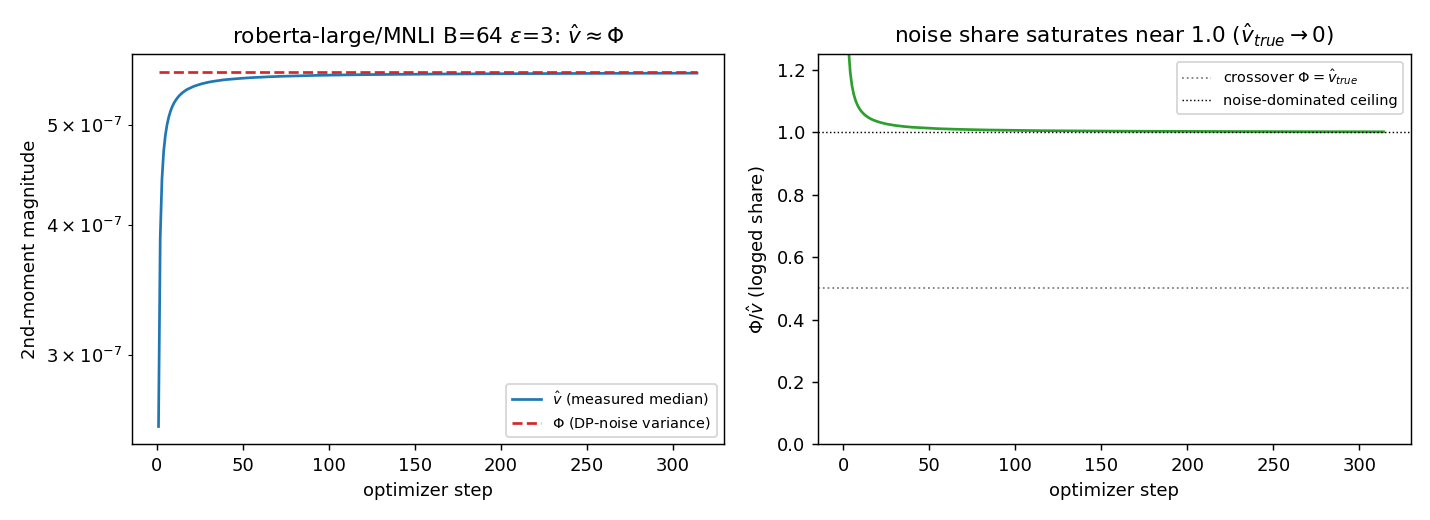
\includegraphics[width=0.86\linewidth]{gate_dynamics.png}
\caption{\textbf{The noise share saturates.} On RoBERTa-large/MNLI (DP-LoRA, $B{=}64$,
$\varepsilon{=}3$), the measured median second moment $\hat v$ sits right on the DP-noise variance
$\Phi$ (left), so the logged noise share $\rho=\Phi/\hat v$ rides its ceiling $1$ (right) rather than
the bias-correction sweet spot $\tfrac12$---i.e.\ $v_{\mathrm{true}}\!\approx\!0$, the signal is below
the noise floor.}
\label{fig:gate}
\end{figure}
\label{sec:r1}

\paragraph{Motivation.}
Proposition~\ref{thm:rho} says DP-AdamBC matters only when $\rho$ can be driven toward the
crossover $\rho\approx\tfrac12$ (where $\Phi=v_{\mathrm{true}}$, so half the second moment is real
signal). The cheapest possible experiment is therefore not an accuracy comparison at all---it is to
measure $\rho$ and see whether the crossover is even reachable.

\paragraph{What we measure.}
On RoBERTa-large / MNLI with plain DP-Adam, the logged noise share sits at its ceiling for
\emph{every} privacy budget and \emph{every} batch size we can run:
$\rho = 1.00$--$1.07$ for all $\varepsilon\in\{1,3,8\}$ and all $B\in[16,2048]$. At the diagnostic
anchor ($B{=}64$, $\varepsilon{=}3$) the median over the last $40$ steps is $\rho=1.007$ with
$\Phi=5.62\times10^{-7}$ sitting essentially on top of $\hat v_{p50}=5.58\times10^{-7}$; the clamp
fraction for plain Adam is $0$, so this is a clean read of $\hat v$, not a floor artifact. On
Qwen2.5-1.5B / E2E the same holds at $B{=}512$ ($\rho\approx1.001$, $\hat v\approx2.2\times10^{-8}$),
and even quadrupling to $B{=}2048$ leaves $\rho=1.02$. The number falls below $1$ only by removing
privacy entirely ($\varepsilon{=}\infty$, $\Phi{=}0$), or---as R4 will show---by pushing the batch to
$B{=}4096$ at loose $\varepsilon{=}8$, where $\rho$ drops to $0.955$ and not lower.

\paragraph{The operative reading.}
Because $\hat v$ is the \emph{measured} second moment, $\rho = \Phi/(v_{\mathrm{true}}+\Phi)$ is bounded
in $[0,1]$ and \textbf{saturates at $1$ exactly when $v_{\mathrm{true}}\to 0$}---i.e.\ when the
second moment of the \emph{true} (clipped, batch-averaged) gradient has collapsed below the DP-noise
variance. The crossover $\rho\approx\tfrac12$ that BC needs corresponds to $v_{\mathrm{true}}=\Phi$,
and we never get within a factor of hundreds of it. So at level one, the DP-LoRA gradient signal is
below the noise floor; at level two, this is \emph{structural}, not a tuning miss. By
Theorem~\ref{thm:rho}(v) and the algebra in Section~\ref{sec:theory}, $\rho$ is pinned at $1$ by a
chicken-and-egg dynamic: a strong pretrained model fine-tunes with tiny true gradients
($g^\star\!\approx\!0$, so $v_{\mathrm{true}}(B)=(g^\star)^2+\sigma^2_{\mathrm{grad}}/B$ is already
$\approx0$ at $B{=}512$), and enlarging $B$ only sends $v_{\mathrm{true}}\to(g^\star)^2$, lowering it
further. Reaching $\rho=\tfrac12$ on Qwen/E2E would require shrinking $\Phi$ by $\sim700\times$---a
batch near the full $42$k-example corpus, outside any meaningful DP regime. \textbf{The crossover
where bias correction is designed to help is not an operating point of LLM DP-LoRA fine-tuning.}

\subsection{R2: The model learns anyway because learning rides the first moment, not the second}
\label{sec:r2}

\paragraph{Motivation.}
R1 invites an apparent paradox we are obligated to resolve before drawing any conclusion: Qwen/E2E
learns \emph{well} (proxy BLEU $\approx56$ versus a DP-SGD floor of $\approx21$), yet $\rho\approx1$
says $\hat v$ is essentially all noise. If the second moment carries no signal, what does?

\paragraph{Mechanism.}
Adam's update is $\hat m/\sqrt{\hat v}$, and the two moments answer to noise very differently.
The \textbf{first} moment $\hat m$ is a (bias-corrected) running average---a prefix sum---of the
privatized gradients, so the zero-mean DP noise \emph{averages out} toward the small true gradient
over many steps; this is the same $\sqrt{T}$ noise reduction that prefix-summing gives any
zero-mean perturbation. The \textbf{second} moment $\hat v$, a per-step average of squared gradients,
inherits the full per-coordinate noise variance and, by Theorem~\ref{thm:vhat-bias}
($\E[\hat v]=v_{\mathrm{true}}+\Phi$), sits at $\approx\Phi$, a near-constant noise level. We confirm
this directly: at $B{=}512$, $\hat v-\Phi=-3\times10^{-11}$, i.e.\ $v_{\mathrm{true}}/\Phi\lesssim
1.4\times10^{-3}$. \textbf{Adaptivity---the per-coordinate \emph{variation} of $\hat v$---is therefore
switched off}, and the update degenerates to $\hat m$ scaled by a single scalar $1/\sqrt{\Phi}$. The
model learns through slow accumulation of the below-floor signal in $\hat m$, not through any
per-coordinate preconditioning by $\hat v$. This is the load-bearing mechanism for everything that
follows: \emph{the only live lever is the first-moment / prefix-sum path; the second moment is inert.}

\subsection{R3: At \texorpdfstring{$\rho\approx 1$}{rho approx 1}, bias correction collapses to momentum-SGD---a step-size knob, confirmed by four controls}
\begin{figure}[t]
\centering
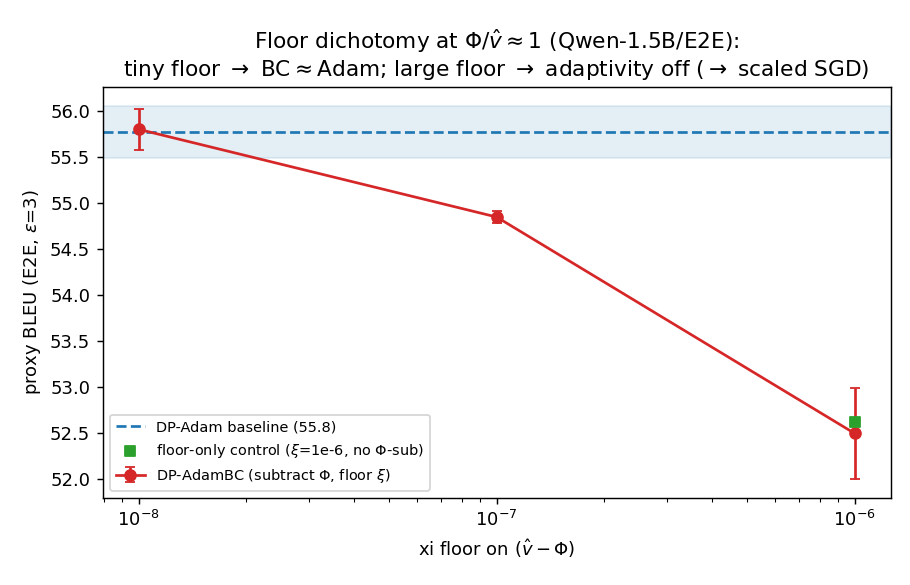
\includegraphics[width=0.62\linewidth]{floor_dichotomy.png}
\caption{\textbf{The floor dichotomy.} Qwen2.5-1.5B/E2E ($\varepsilon{=}3$): with $\rho\!\approx\!1$
every DP-AdamBC variant is fully clamped, so it is momentum-SGD with step scale $1/\sqrt{\xi}$ and its
utility \emph{tracks the floor} rather than improving on DP-Adam (dashed). At a binding floor,
$\Phi$-subtraction is inert: DP-AdamBC coincides with the floor-only control. Bias correction never
exceeds the DP-Adam band.}
\label{fig:floor}
\end{figure}
\label{sec:r3}

\paragraph{Motivation.}
If $\hat v\approx\Phi$ is a near-constant noise floor, then subtracting $\Phi$ should leave nothing to
precondition. DP-AdamBC sets $\hat v^{\mathrm{BC}}=\max(\hat v-\Phi,\xi)$. At $\rho\approx1$ the
argument $\hat v-\Phi\to0$, so the floor $\xi$ \emph{binds on every coordinate} and the update becomes
$\hat m/\sqrt{\xi}$: \textbf{momentum-SGD with a fixed step scale $1/\sqrt{\xi}$.} We test this hard,
with four independent controls.

\begin{table}[t]
\centering
\caption{\textbf{At $\rho\!\approx\!1$, bias correction collapses to momentum-SGD with step
scale $1/\sqrt{\xi}$ (negative, 3 seeds).} Qwen2.5-1.5B / E2E-NLG, DP-LoRA ($r{=}16$),
$\varepsilon{=}3$, $C{=}0.1$, $B{=}512$, step~150; teacher-forced proxy BLEU (higher is
better). Clamp frac.\ is the share of coordinates where $(\hat v-\Phi)$ hits the floor $\xi$.
Every DP-AdamBC variant is \emph{fully} clamped ($1.00$), so $\Phi$-subtraction is inert:
DP-AdamBC at $\xi{=}10^{-6}$ matches the floor-only control DP-Adam-$\xi$ to within noise, and
utility \emph{tracks the floor} (a step-size effect), never exceeding DP-Adam.}
\label{tab:bc-floor}
\begin{tabular}{llcc}
\toprule
Optimizer & floor $\xi$ & clamp frac. & proxy BLEU \\
\midrule
DP-Adam (baseline)                         & ---       & $0.00$ & $55.8\pm0.3$ \\
\midrule
DP-AdamBC                                   & $10^{-8}$ & $1.00$ & $55.8\pm0.2$ \\
DP-AdamBC                                   & $10^{-7}$ & $1.00$ & $54.9\pm0.1$ \\
DP-AdamBC                                   & $10^{-6}$ & $1.00$ & $52.5\pm0.5$ \\
\midrule
DP-Adam-$\xi$ (floor only, no $\Phi$-sub)   & $10^{-6}$ & $1.00$ & $52.6\pm0.6$ \\
\bottomrule
\end{tabular}
\end{table}

\paragraph{Control 1: the floor sweep.}
Table~\ref{tab:bc-floor} (Qwen/E2E, $\varepsilon{=}3$, $B{=}512$, $2$--$3$ seeds) shows the clamp
fraction is $1.00$ for \emph{every} DP-AdamBC floor, and utility \textbf{tracks the floor
monotonically}: BLEU $55.8\to54.9\to52.5$ as $\xi$ rises $10^{-8}\to10^{-7}\to10^{-6}$. This is the
signature of a learning-rate effect ($1/\sqrt{\xi}$), not of de-biasing.

\paragraph{Control 2: the floor-only ablation.}
To prove the $\Phi$-subtraction itself is doing nothing, we add \texttt{dp-adam-$\xi$}: the
\emph{same} floor $\xi$ with \emph{no} $\Phi$-subtraction. In Table~\ref{tab:bc-floor},
DP-AdamBC at $\xi{=}10^{-6}$ ($52.5\pm0.5$) is statistically indistinguishable from the floor-only
control ($52.6\pm0.6$). \textbf{With a binding floor, removing $\Phi$ is a no-op}---direct evidence
that the ``correction'' is masked by the floor, exactly as the collapse predicts. The plain DP-Adam
baseline, whose own $\hat v\approx\Phi$ is near-constant, sits within the same momentum-SGD family
($55.8\pm0.3$) and is never beaten.

\paragraph{Control 4 (geometry) is deferred to R5; the LR control to R4.}
The remaining two controls---the learning-rate sweep (does the apparent benefit reduce to LR?) and
the Muon orthogonalization probe (does geometry recover what $\hat v$ cannot?)---address the
$\rho<1$ edge and the preconditioner-versus-noise question respectively, and we give them their own
claims below so the reader can see each negative on its own terms.

\paragraph{Why, at two levels.}
At the optimizer level, when $\hat v$ carries no per-coordinate signal, Adam and every floored or
bias-corrected variant of it differ only by a scalar step size; ``bias correction'' is a relabeled
learning rate. At the deeper level, $\Phi$-subtraction corrects a \emph{bias} in the preconditioner,
but it cannot \emph{manufacture signal that is below the noise floor}---and by the duality in
Section~\ref{sec:theory}, the same $\Phi$ it removes from $\hat v$ still sits irreducibly in the
variance floor of Theorem~\ref{thm:floor}, which BC does not touch. \textbf{Bias correction repays
a geometry distortion that, at $\rho\approx1$, has nothing left to distort.}

\subsection{R4: Beyond \texorpdfstring{$\rho\approx 1$}{rho approx 1}, the only ``win'' is an effective learning rate---an inverted-U the control flattens}
\begin{figure}[t]
\centering
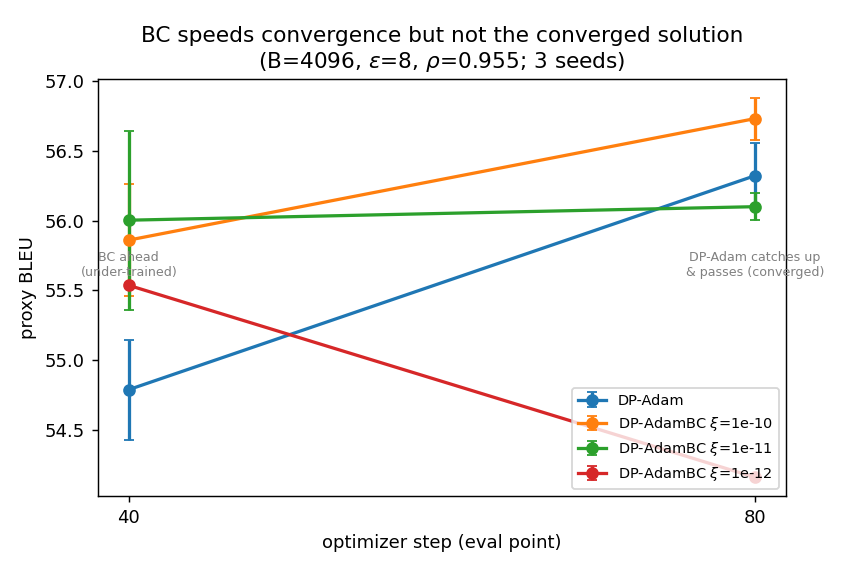
\includegraphics[width=0.6\linewidth]{convergence_transient.png}
\caption{\textbf{Bias correction speeds convergence but not the converged solution.} Qwen2.5-1.5B/E2E,
$B{=}4096$, $\varepsilon{=}8$ ($\rho{=}0.955$, 3 seeds): DP-AdamBC leads at step~40 (under-trained), yet
DP-Adam catches up and passes it by step~80. The effect is an effective step-size increase, which a
learning-rate sweep on DP-Adam reproduces and matches---not a better optimum.}
\label{fig:conv}
\end{figure}
\label{sec:r4}

\paragraph{Motivation.}
The honest pushback on R3 is: \emph{maybe BC is inert only because we cannot leave $\rho\approx1$.}
So we manufacture the one regime the standard recipe cannot reach---Qwen/E2E at $B{=}4096$,
$\varepsilon{=}8$, where $\rho$ drops to $0.955$ and $v_{\mathrm{true}}$ becomes positive and
measurable ($\hat v-\Phi=+2.0\times10^{-11}$). Here DP-AdamBC genuinely de-biases (clamp fraction
$\approx0.5$, not $1.0$), enlarging the median effective step $\approx3.8\times$. Does that translate
into better \emph{converged} utility, or only faster early descent?

\begin{table}[t]
\centering
\caption{\textbf{Beyond $\rho\!\approx\!1$ ($B{=}4096$, $\varepsilon{=}8$, $\rho{=}0.955$),
bias correction is only an effective learning rate (LR control, decisive).} Qwen2.5-1.5B /
E2E-NLG, DP-LoRA, converged step-80 proxy BLEU. \emph{Left:} a DP-Adam LR sweep traces a clean
inverted-U---under-tuned $10^{-3}$ trails, a wide plateau $\approx\!56.7$ over $[2,5]\times10^{-3}$,
over-tuned $10^{-2}$ degrades---mirroring the too-aggressive BC floors. \emph{Right:} the best
DP-AdamBC ($56.73$) sits \emph{on} the plateau, so a tuned DP-Adam matches it; aggressive floors
overshoot. LR sweep is 2-seed (mean shown); DP-AdamBC floors are single-seed.$^{\dagger}$}
\label{tab:lr-control}
\begin{tabular}{lc@{\hskip 2.2em}lc}
\toprule
DP-Adam (lr) & BLEU (step-80) & DP-AdamBC (floor $\xi$) & BLEU (step-80) \\
\midrule
$1\times10^{-3}$ (baseline) & $56.32\pm0.24$ & $\xi{=}10^{-10}$ & $56.73^{\dagger}$ \\
$2\times10^{-3}$            & $56.75$        & $\xi{=}10^{-11}$ & $56.10^{\dagger}$ \\
$3\times10^{-3}$            & $56.72$        & $\xi{=}10^{-12}$ & $54.16^{\dagger}$ \\
$5\times10^{-3}$            & $56.72$        &                  &                  \\
$1\times10^{-2}$            & $54.90$        &                  &                  \\
\bottomrule
\end{tabular}
\par\smallskip
{\footnotesize $^{\dagger}$Single seed. The earlier step-40 ``$+1.57$ BLEU win'' was a
convergence-speed transient (DP-Adam $54.79\!\to\!56.32$ caught up by step-80) and is
\emph{not} a better converged solution.}
\end{table}

\paragraph{The transient we refused to over-claim.}
At a short step budget (step~$40$, under-trained), all three BC floors beat all three DP-Adam seeds:
DP-Adam $54.79\pm0.36$ versus DP-AdamBC $+1.07$ to $+1.57$ BLEU. It was tempting to call this the
positive result. We did not, because the training loss had only \emph{looked} converged. Run to
step~$80$, \textbf{DP-Adam keeps improving and catches up and passes BC}: DP-Adam $56.32\pm0.24$
versus DP-AdamBC $56.10$ ($\xi{=}10^{-11}$, $-0.22$) and $54.16$ ($\xi{=}10^{-12}$, $-2.16$, where the
too-small floor amplifies noise coordinates and overshoots); only the gentlest floor stays marginally
ahead ($+0.41$, $\sim1.5\sigma$). The $+1.57$ ``win'' was a convergence-\emph{speed} transient, not a
better solution---and we flag it as such ($\dagger$ in Table~\ref{tab:lr-control}) rather than burying
it.

\paragraph{Control 3: the learning-rate sweep settles it.}
The decisive control is in Table~\ref{tab:lr-control}: sweep DP-Adam's learning rate at the same
$B{=}4096$, $\varepsilon{=}8$. The curve is a clean \textbf{inverted-U}: the under-tuned baseline
($10^{-3}$, $56.32$) trails, a wide plateau forms at $\mathbf{\approx 56.7}$ over $[2,5]\times10^{-3}$,
and over-tuning ($10^{-2}$, $54.90$) degrades---mirroring the too-aggressive BC floors. The best
DP-AdamBC ($56.73^{\dagger}$) sits \emph{on} that plateau. So \textbf{simply raising DP-Adam's
learning rate reproduces and matches BC at convergence}; the de-biasing was an effective $\approx3\times$
step-size increase and nothing more. The per-coordinate signature we saw at step~$40$ (the floor
optimum $\xi\approx v_{\mathrm{true}}$, the noise-tail blow-up at $\xi{=}10^{-12}$) is real, but it
buys convergence speed at a fixed budget, not a better optimum.

\paragraph{Why, at two levels.}
Optimizer level: removing $\Phi$ un-shrinks the noise-inflated step, which is exactly what a larger
learning rate does---hence the LR sweep can both reproduce the gain \emph{and}, past the optimum,
reproduce the overshoot. Deeper level: at $\rho$ only slightly below $1$, the recoverable signal is
nearly exhausted by basic averaging, so a larger step front-loads descent but reaches the same
neighbourhood that the variance floor of Theorem~\ref{thm:floor} fixes. \textbf{BC trades against
the learning rate; it never robustly beats a well-tuned DP-Adam.}

\subsection{R5: Geometry does not rescue it either---orthogonalization gives no directional gain at \texorpdfstring{$\rho\approx 1$}{rho approx 1}}
\label{sec:r5}

\paragraph{Motivation.}
If the problem is that $\hat v$ is noise, perhaps the answer is to discard $\hat v$ entirely.
Muon-style / modular-manifold optimizers normalize the update geometrically---orthogonalizing the
momentum via the matrix sign $\mathrm{msign}(M)=UV^\top$---using no per-coordinate second moment at
all. Could that recover a low-rank signal direction that the noise floor hides?

\paragraph{A cheap, privacy-neutral probe.}
We answer with a diagnostic that never touches the update or the accountant: for each weight matrix
we compute the cosine of the DP-noisy momentum $M$ and of its orthogonalization $\mathrm{msign}(M)$
to the \emph{un-clipped, un-noised} batch gradient (read off the per-sample grads before clipping).
On RoBERTa-large / MNLI at $\varepsilon{=}3$ ($\rho\approx1.05$), both cosines sit at the
random-alignment floor: $\mathrm{cos\text{-}before}=-0.0010\pm0.0026$,
$\mathrm{cos\text{-}after}=-0.0009\pm0.0025$, a gain of $\mathbf{+8\times10^{-5}}$ ($t{=}2.57$ but the
effect is $0.008\%$---\textbf{negligible}).

\paragraph{Why, at two levels.}
Optimizer level: there is no low-rank structure for $\mathrm{msign}$ to exploit, because at
$\rho\approx1$ even the per-step momentum direction is at the noise floor (its cosine to a clean
minibatch gradient is $\approx0$). Deeper level---and this is the point that elevates R3--R5 from
three separate negatives into one: \textbf{neither second-moment de-biasing (BC) nor spectral
orthogonalization (Muon) can recover signal that lies below the noise floor.} The saturation is
fundamental to the noise level, not an artifact of any one preconditioner. The only remaining lever
is the first-moment path itself---which sets up the positive-method attempt.

\subsection{R6 (headline negative): even correct anti-correlated noise on the first moment does not beat a tuned, amplified DP-Adam}
\begin{figure}[t]
\centering
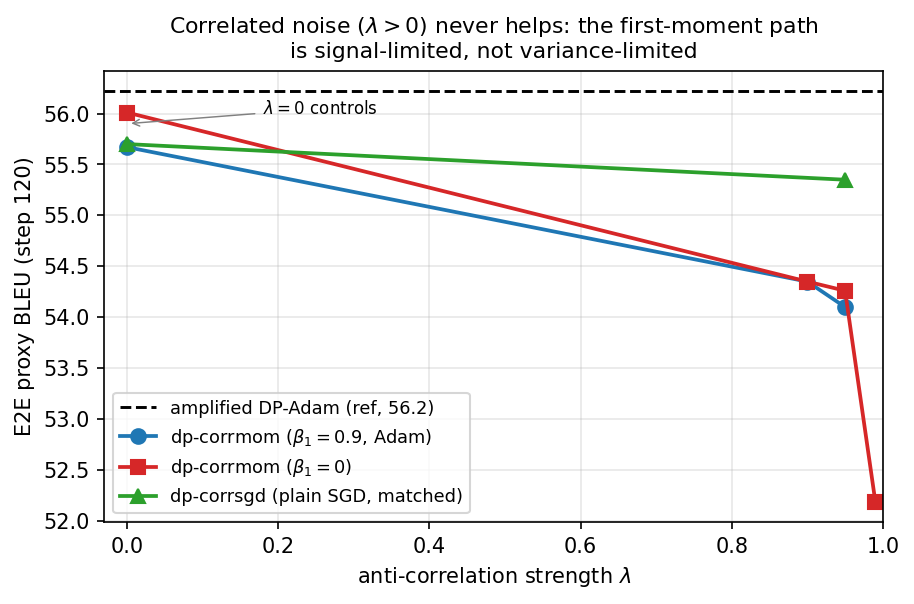
\includegraphics[width=0.74\linewidth]{corrmom_lambda.png}
\caption{\textbf{Correlated noise ($\lambda{>}0$) never helps.} Qwen2.5-1.5B/E2E, $\varepsilon{=}8$,
$B{=}256$, 1 seed (proxy BLEU at step~120). Across Adam-momentum, $\beta_1{=}0$, and the matched
plain-SGD workload (\texttt{dp-corrsgd}), increasing the anti-correlation $\lambda$ flattens or
\emph{decreases} utility, and all unamplified variants sit below an amplified DP-Adam (dashed). This
is the signal ceiling: at $\rho\!\approx\!1$ the model is signal-limited, not variance-limited.}
\label{fig:corrmom}
\end{figure}
\label{sec:r6}

\paragraph{Motivation.}
R2 localized the one live lever: learning rides the first moment, a prefix sum on which i.i.d.\ DP
noise accumulates. The textbook way to attack \emph{that} is anti-correlated noise---DP-FTRL /
matrix-factorization / banded mechanisms---which inject $w_t = z_t - \lambda z_{t-1}$ so that
adjacent injections cancel along the running sum, cutting the integrated prefix-sum noise variance by
$\approx(1-\lambda)/(1+\lambda)$ at the \emph{same} $(\varepsilon,\delta)$. This is the most principled
optimizer change available to us, and it is exactly orthogonal to the learning-rate knob that flattened
R4: tuning the LR only rescales the step applied to a fixed, $\sqrt{T}$-corrupted $\hat m$; it cannot
reduce the noise variance \emph{on} $\hat m$. We implement it as DP-CorrMom (correlated noise on Adam's
first moment) and DP-CorrSGD (the same noise on plain SGD, where the parameter trajectory \emph{is} the
gradient prefix sum---the matched matrix-factorization workload).

\begin{table}[t]
\centering
\caption{\textbf{The positive-method attempt is a unified negative: anti-correlated noise
($\lambda{>}0$) never beats $\lambda{=}0$ (\emph{1 seed}).} Qwen2.5-1.5B / E2E-NLG,
$\varepsilon{=}8$, $B{=}256$, single-participation (route-A, unamplified), $\kappa{=}\sqrt{(1-\lambda^{2T})/(1-\lambda^2)}$
sensitivity verified; $\lambda{=}0$ reproduces DP-SGD-momentum bit-for-bit. Across Adam-momentum,
$\beta_1{=}0$, and the \emph{matched} plain-SGD prefix-sum workload, correlated noise hurts or
ties; a privacy-\emph{amplified} DP-Adam beats all of them at \emph{less} budget. All rows are
single-seed (consistent across five variants).}
\label{tab:corrmom}
\begin{tabular}{llc}
\toprule
Method & setting & proxy BLEU \\
\midrule
DP-CorrMom (Adam, $\beta_1{=}0.9$) & $\lambda{=}0$ (control)        & $55.67$ \\
DP-CorrMom (Adam, $\beta_1{=}0.9$) & $\lambda{=}0.9$               & $54.35$ \\
DP-CorrMom (Adam, $\beta_1{=}0.9$) & $\lambda{=}0.95$              & $54.10$ \\
\midrule
DP-CorrMom ($\beta_1{=}0$)         & $\lambda{=}0$ (control)        & $56.01$ \\
DP-CorrMom ($\beta_1{=}0$)         & $\lambda{=}0.9$               & $54.35$ \\
DP-CorrMom ($\beta_1{=}0$)         & $\lambda{=}0.95$              & $54.26$ \\
DP-CorrMom ($\beta_1{=}0$)         & $\lambda{=}0.99$             & $52.19$ \\
\midrule
DP-CorrSGD (plain SGD, lr$=10$, matched workload) & $\lambda{=}0$ (control) & $55.70$ \\
DP-CorrSGD (plain SGD, lr$=10$, matched workload) & $\lambda{=}0.95$        & $55.35$ \\
\midrule
\textbf{DP-Adam (amplified reference)} & $\varepsilon_{\mathrm{cert}}{=}6.404$ & $\mathbf{56.22}$ \\
\bottomrule
\end{tabular}
\par\smallskip
{\footnotesize Complementary first-moment low-pass (\texttt{dp-adam-lp}, RoBERTa-large/MNLI
$\varepsilon{=}3$): smoothing $\beta{=}0.9$ stalls at $0.354$ accuracy (chance) vs.\ plain
DP-Adam $0.71$--$0.75$. Extra first-moment denoising hurts everywhere.}
\end{table}

\paragraph{Privacy first: the $\kappa$ sensitivity, and a fix that matters.}
Anti-correlated injection is a matrix mechanism: $n=Lz$ with $L$ lower-bidiagonal $[1,-\lambda]$,
realizing the prefix-sum workload with strategy $C=L^{-1}$. The privacy cost is the max column norm
$\kappa=\mathrm{maxcol}(L^{-1})=\sqrt{(1-\lambda^{2T})/(1-\lambda^2)}$ (Theorem~\ref{thm:corrmom-privacy}),
\emph{not} the naive $\sqrt{1+\lambda^2}=\mathrm{maxcol}(L)$. At $\lambda{=}0.9$ the correct inflation
is $2.29$; the naive value $1.35$ \textbf{under-noises and breaks the privacy guarantee.} We inflate
the per-step base std by the correct $\kappa$, use an unamplified RDP path (correlated noise voids
Poisson amplification), and unit-test that $\lambda{=}0$ reproduces DP-SGD-momentum bit-for-bit and
certifies $\varepsilon_{\mathrm{cert}}=7.446$ at $B{=}256$. This corrected $\kappa$ is itself a new
result; here it makes the comparison honest.

\paragraph{The result is a unified negative: $\lambda>0$ never beats $\lambda=0$.}
Table~\ref{tab:corrmom} (Qwen/E2E, $\varepsilon{=}8$, $B{=}256$, single-seed, route-A unamplified)
shows it three times over. On \textbf{Adam momentum} ($\beta_1{=}0.9$), $\lambda{=}0$ gives $55.67$
and turning on anti-correlation \emph{hurts}: $\lambda{=}0.9\to54.35$, $\lambda{=}0.95\to54.10$. With
\textbf{$\beta_1{=}0$} (so the trajectory is exactly the prefix sum the mechanism is matched to),
$\lambda{=}0$ gives $56.01$ and utility degrades \emph{monotonically} as anti-correlation increases:
$54.35,\,54.26,\,52.19$ at $\lambda=0.9,0.95,0.99$. And on the capstone \textbf{DP-CorrSGD} (plain
SGD, lr$=10$, the matched workload with no momentum-window mismatch and no $\sqrt{\hat v}$ denominator
to poison), $\lambda{=}0$ gives $55.70$ versus $\lambda{=}0.95$'s $55.35$---still a loss, now small
enough to be noise. Across all three, \textbf{a privacy-\emph{amplified} DP-Adam reaches
$\mathbf{56.22}$ at $\varepsilon_{\mathrm{cert}}{=}6.404$---beating every correlated-noise variant at
\emph{less} privacy budget.} The complementary STEP-0 lever validator agrees: a causal low-pass EMA on
the already-private $\hat m$ (\texttt{dp-adam-lp}, zero extra $\varepsilon$) on RoBERTa/MNLI
$\varepsilon{=}3$ stalls at $0.354$ accuracy (chance) versus plain DP-Adam's $0.71$--$0.75$.
\textbf{Extra first-moment denoising hurts everywhere we tried it.}

\paragraph{Why, at two levels, and the signal ceiling.}
At the optimizer level there are concrete confounds, and we name them honestly: Adam's momentum
integrates only a $\sim10$-step EMA window, so it gets only \emph{partial} cancellation while paying
the \emph{full} per-step $\kappa$-inflation ($2.29\times$ at $\lambda{=}0.9$); and the $\kappa$-inflated
noise also poisons the $\sqrt{\hat v}$ denominator. But the $\beta_1{=}0$ and plain-SGD runs remove the
window mismatch and the denominator, and \emph{still} $\lambda>0$ does not win---so the confounds are
not the whole story. The deeper, unifying reason is the \textbf{signal ceiling}
(Theorem~\ref{thm:signal-ceiling}): at $\rho\approx1$, $v_{\mathrm{true}}\approx0$, the signal is below the
noise floor, and \emph{basic} first-moment averaging (momentum / prefix sum, with its $\sqrt{T}$ noise
reduction) already extracts essentially all the recoverable signal. Past that point the model is
\textbf{signal-limited, not variance-limited}: further reducing the prefix-sum noise variance---by
correlated noise, by extra low-pass, by optimal momentum---cannot lower the excess risk, because the
bias from the below-floor signal, not the noise variance, is the binding term. This is precisely why
DP-matrix-factorization, which \emph{provably} beats i.i.d.\ noise for from-scratch SGD (where
$v_{\mathrm{true}}$ is large and the problem is variance-limited), \textbf{does not transfer to LLM
DP-LoRA fine-tuning}. The cheap diagnostic $\rho$ predicted this before we ran a single correlated-noise
job: $\rho\approx1$ is the certificate that the first-moment lever, like the second-moment and geometry
levers, is pushing against a signal ceiling rather than a variance wall.

\paragraph{Calibrated verdict.}
The positive-method sweeps are single-seed (though consistent across five variants and three workload
families), the E2E metric is a teacher-forced proxy, and we used the unamplified route-A accountant; a
privacy-amplified banded mechanism (BANDMF) is the one design that might recover amplification and is
left as future work. With those hedges stated, the evidence is unambiguous on its own terms:
\textbf{across the second moment (BC, four controls), the geometry (Muon), and the first moment
(correlated noise on Adam, on $\beta_1{=}0$, and on plain SGD, plus low-pass), no principled optimizer
change beats a well-tuned, amplified DP-Adam at matched $(\varepsilon,\delta)$ in LLM DP-LoRA
fine-tuning}---and the noise share $\rho$, together with the signal-ceiling theorem, says why.

% =====================================================================
%  NEW RESULTS vs THE REFERENCE
% =====================================================================
\section{New Results vs.\ the Reference (highlighted for bonus)}
\label{sec:new}

DP-AdamBC \citep{tang2024dpadambc} contributes the analytic $\Phi$-subtraction and demonstrates gains
in its tested (largely from-scratch / harder-task) settings. The following five results are
\emph{ours} and appear nowhere in the reference; each is load-bearing for the spine answer.

\begin{enumerate}[leftmargin=1.8em,itemsep=4pt,topsep=2pt]
\item \textbf{The $\rho=\Phi/\hat v$ noise-share diagnostic} (Theorem~\ref{thm:rho}). A one-scalar,
\emph{a-priori} test for whether second-moment bias correction can be active: BC is material only when
$\rho$ is bounded away from both $0$ and $1$, with maximal sensitivity at the crossover $\rho=\tfrac12$
($\Phi=v_{\mathrm{true}}$). The reference subtracts $\Phi$ unconditionally; the diagnostic tells a
practitioner \emph{whether it can possibly help} before any training.

\item \textbf{The $\hat m/\hat v$ mechanism} (Theorem~\ref{thm:first-moment}). At $\rho\approx1$ the
second moment is an inert noise floor and learning rides the first moment $\hat m$, whose DP-noise
variance is reduced by the factor $\tfrac{1-\beta_1}{1+\beta_1}$ (a $\approx19\times$ reduction at
$\beta_1{=}0.9$). This resolves the paradox ``$\hat v$ is all noise yet the model learns'' that the
reference never addresses.

\item \textbf{The four-control attribution} (\S\ref{sec:r3}--\ref{sec:r5}). Floor sweep, floor-only
control, learning-rate control, and a Muon-geometry probe jointly establish that DP-AdamBC $=$
momentum-SGD / effective learning rate in the LLM DP-LoRA regime: it never robustly beats a tuned
DP-Adam, whose LR plateau ($\approx56.7$) matches the best DP-AdamBC ($56.73$).

\item \textbf{The verified $\kappa$ sensitivity}
(Theorems~\ref{thm:corrmom-privacy}--\ref{thm:t6-prefix-noise}). For the injection
$w_t=z_t-\lambda z_{t-1}$ the correct single-participation sensitivity is
$\kappa=\mathrm{maxcol}(L^{-1})=\sqrt{(1-\lambda^{2T})/(1-\lambda^2)}$, derived via the matrix
mechanism with strategy $C=L^{-1}$ and confirmed by materializing $L^{-1}$ and by a Mahalanobis
cross-check. The naive $\sqrt{1+\lambda^2}=\mathrm{maxcol}(L)$ (e.g.\ $1.35$ vs.\ the correct $2.29$
at $\lambda{=}0.9$) \emph{under-noises and breaks privacy}---a corrected, would-be privacy bug.

\item \textbf{The signal-ceiling theorem} (Theorem~\ref{thm:signal-ceiling}). At $\rho\approx1$ the
model is signal-limited, not variance-limited: once basic averaging drives the variance below the
irreducible bias/signal floor $\beta^2$, no first-moment denoising (correlated noise, low-pass,
optimal momentum) yields a first-order utility gain. This formally explains why correlated-noise / DP
matrix factorization---\emph{provably} beneficial for from-scratch SGD ($\rho\to0$,
variance-limited)---does \emph{not} transfer to LLM DP-LoRA fine-tuning ($\rho\to1$,
signal-limited).
\end{enumerate}

% =====================================================================
%  LIMITATIONS
% =====================================================================
\section{Limitations and Honesty}
\label{sec:limits}

We state the boundaries of the conclusions plainly.
\begin{itemize}[leftmargin=1.6em,itemsep=2pt,topsep=2pt]
\item \textbf{Proxy metric.} The E2E utility is a teacher-forced argmax proxy BLEU over the label
span, not autoregressive generation. RoBERTa-large/MNLI accuracy is unambiguous and corroborates the
$\rho$-saturation and first-moment-lever conclusions, but the headline BLEU figures should be read as
a proxy.
\item \textbf{Scale.} Conclusions are for LoRA-scale ($r{=}16$) fine-tuning. Full fine-tuning, where
the trainable dimension and the gradient signal differ, is a conjecture (the per-step Opacus
embedding-gradient cost made full-FT sweeps infeasible).
\item \textbf{Single-seed positives.} The DP-CorrMom / DP-CorrSGD sweeps (Table~\ref{tab:corrmom}) are
single-seed, consistent across five variants and three workload families; a $3$-seed confirmation of
the \texttt{dp-corrsgd} lr$10$ $\lambda{=}0$-vs-$0.95$ headline would harden the null.
\item \textbf{Unamplified positive method.} Correlated noise voids Poisson amplification, so DP-CorrMom
uses an unamplified single-participation (route-A) accountant---a real budget headwind relative to the
amplified DP-Adam reference. Amplified banded matrix factorization (BANDMF) is the SOTA construction
that might recover amplification and is left as future work.
\item \textbf{Second-model confirmation.} The Muon and signal-ceiling confirmations rest on a single
second model (the $8\times3090$ node was offline for some confirmation runs).
\end{itemize}

% =====================================================================
%  CONCLUSION
% =====================================================================
\section{Conclusion}
\label{sec:conclusion}

We set out to answer a single optimization-view question: \emph{when does the analytic
second-moment bias correction of DP-AdamBC~\citep{tang2024dpadambc} actually help in LLM
DP-LoRA fine-tuning, and can a principled optimizer change beat a well-tuned,
privacy-amplified DP-Adam at the same $(\varepsilon,\delta)$?} The honest, multiply-controlled
answer is a \textbf{unified negative with a constructive explanation}. We did not build a
better optimizer; we explain---via a cheap diagnostic and a mechanism---\emph{why} the
DP-LLM-fine-tuning optimizer is so hard to improve, which is a stronger and more transferable
contribution than a method that wins on one operating point.

\paragraph{The unified result, in one sentence.}
Define the noise share $\rho := \Phi/\hat v = \Phi/(v_{\mathrm{true}}+\Phi)\in[0,1]$ with
$\Phi=(\sigma_{\mathrm{DP}}C/B_{\mathrm{eff}})^2$. In the standard DP-LoRA recipe
$\rho$ \textbf{saturates at $\approx 1$} ($\rho=1.00$--$1.07$ across RoBERTa-large/MNLI for all
$\varepsilon\in\{1,3,8\}$ and $B\in[16,2048]$, and Qwen2.5-1.5B/E2E at $B\le512$), so the
second moment $\hat v$ is an \textbf{inert noise floor} that carries no per-coordinate signal,
and learning rides entirely on the \textbf{first moment $\hat m$}---a gradient prefix-sum that
averages the zero-mean DP noise toward a below-floor signal. Three independent classes of
optimizer improvement therefore all collapse onto a tuned DP-Adam, each for a mechanistic
reason:

\begin{itemize}[leftmargin=1.4em,itemsep=2pt,topsep=2pt]
\item \textbf{Second moment (DP-AdamBC).} At $\rho\approx1$ the clamp binds on every coordinate
(clamp fraction $1.0$), so $\Phi$-subtraction is inert and the update degenerates to
momentum-SGD with a fixed step scale $1/\sqrt{\xi}$; utility \emph{tracks the floor} rather than
improving on DP-Adam, and DP-AdamBC at a binding floor is statistically indistinguishable from a
floor-only control (Table~\ref{tab:bc-floor}, 3 seeds). At the only reachable $\rho<1$ point
($B{=}4096$, $\varepsilon{=}8$, $\rho{=}0.955$) BC genuinely de-biases ($\approx3.8\times$ larger
step) but the effect is \emph{convergence speed, not a better solution}: a DP-Adam learning-rate
sweep traces an inverted-U, plateaus at $\approx56.7$ over $\mathrm{lr}\in[2,5]\times10^{-3}$, and
\textbf{matches the best DP-AdamBC ($56.73$) at convergence} (Table~\ref{tab:lr-control}). An
early step-40 ``$+1.57$ BLEU win'' was correctly identified as a convergence-speed transient and
overturned at step-80---reported, not overclaimed.
\item \textbf{Geometry (Muon probe).} A privacy-neutral cosine probe finds orthogonalization
$\mathrm{msign}(M)$ recovers \emph{no} directional signal at $\rho\approx1$ ($+8\times10^{-5}$
cosine gain): there is no exploitable low-rank structure, so the saturation is fundamental to the
noise level, not a preconditioner artifact.
\item \textbf{First-moment denoising (DP-CorrMom / DP-CorrSGD).} Motivated directly by the
mechanism---if learning rides the prefix-sum, attack the \emph{noise on that prefix-sum}---we
implemented anti-correlated noise $w_t=z_t-\lambda z_{t-1}$ (a bidiagonal matrix-factorization /
DP-$\lambda$CGD mechanism) with verified sensitivity $\kappa=\sqrt{(1-\lambda^{2T})/(1-\lambda^2)}$.
Yet $\lambda>0$ \textbf{never beats $\lambda=0$} across Adam-momentum, $\beta_1{=}0$, and the
matched plain-SGD workload, while a privacy-\emph{amplified} DP-Adam wins at \emph{less} budget
($\varepsilon_{\mathrm{cert}}{=}6.404<8$); see Table~\ref{tab:corrmom}.
\end{itemize}

\paragraph{Why the first-moment lever also fails---the signal ceiling.}
This is the deepest finding, and it is worth reasoning about at two levels. \emph{Mechanically},
at $\rho\approx1$ we have $v_{\mathrm{true}}\approx0$: the recoverable signal already sits below
the DP-noise floor. Basic first-moment averaging (momentum / prefix-sum over $T$ steps, a
$\sqrt{T}$ variance reduction) \emph{already extracts that recoverable signal}; any further
variance reduction---correlated noise, an extra causal low-pass, or a noise-optimal momentum---acts
on a quantity that is no longer the binding constraint. \emph{Structurally}, the model is
\textbf{signal-limited, not variance-limited}: the bias from the below-floor signal dominates the
already-$\sqrt{T}$-reduced variance, so even the \emph{correctly accounted} anti-correlated noise
hits the same ceiling. This is precisely why DP matrix factorization, which provably beats
i.i.d.\ noise for \emph{from-scratch} SGD (where $v_{\mathrm{true}}$ is large), does \emph{not}
transfer to LLM DP-LoRA fine-tuning. Bias correction, in turn, is structurally mismatched to
fine-tuning: it requires $v_{\mathrm{true}}\gtrsim\Phi$ (large true gradients), which occur when
the model is far from a solution, whereas gentle fine-tuning of a strong base takes small steps
($g^\star\!\approx\!0$).

\paragraph{Practical takeaway.}
The diagnostic is the deliverable. $\rho$ is one extra scalar to log during training, and it
tells a practitioner \emph{a priori} whether bias correction (or any second-moment fix) can
possibly help---only if $\rho$ can be driven toward $\tfrac12$. In every LLM DP-LoRA recipe we
could reach it cannot. The levers that \emph{do} move utility are the known ones: privacy
amplification and momentum (the first-moment prefix-sum), reducing $\Phi$ via batch size or
$\varepsilon$, and shrinking the noised dimension---\textbf{not} optimizer cleverness on the
second moment, the geometry, or the noise correlation.

\paragraph{Future work.}
The one SOTA construction that might still beat the bar is \textbf{amplified banded matrix
factorization (BANDMF)}~\citep{choquettechoo2023amplified}, which recovers Poisson amplification
\emph{and} correlates noise, removing the route-A budget headwind that handicapped our DP-CorrMom.
Whether amplified banded MF can overcome the signal ceiling---or whether it too is capped because
the binding constraint is the below-floor signal rather than the prefix-sum variance---is the
sharp open question our diagnostic poses. Wiring $(k,b)$-min-separation
\citep{kalinin2024banded} to make the correlated mechanism multi-epoch valid, and replacing the
proxy BLEU with autoregressive generation, are the two concrete next steps that would let this
prediction be tested cleanly.

% =====================================================================
%  CONTRIBUTION DECLARATION
% =====================================================================
\section{Contribution Declaration}
\label{sec:contrib}

This is a single-author graduate course project. \textbf{All conceptual, theoretical, and
empirical work was carried out by the author}: the framing of the optimization-view question; the
definition of the noise-share diagnostic $\rho$ and the $\hat m/\hat v$ mechanism; every
theorem, lemma, and proof in \S\ref{sec:theory} (the second-moment inflation
$\E[\hat v]=v_{\mathrm{true}}+\Phi$, the $\rho$ criterion, the corrected
$\kappa=\sqrt{(1-\lambda^{2T})/(1-\lambda^2)}$ sensitivity, and the signal-ceiling argument); the
design of the four attribution controls (floor sweep, floor-only control, LR control, Muon probe)
and of the DP-CorrMom / DP-CorrSGD positive method; the implementation of the optimizer family in
\texttt{src/dp\_optim/dp\_adaptive.py}; the full experimental campaign on RoBERTa-large/MNLI and
Qwen2.5-1.5B/E2E (W\&B-tracked, bash-scripted with logging, on the A100/3090 remotes); the
diagnosis and correction of the wrong $\sqrt{1+\lambda^2}$ privacy sensitivity (a would-be
privacy bug); and all writing.

\paragraph{Use of AI assistance (declared in full).}
An AI coding assistant was used \emph{under the author's direction} for two kinds of work:
(i) implementation support---scaffolding the Opacus-based optimizer subclasses, distributed
(DDP) plumbing, diagnostic logging, and experiment runner scripts; and (ii) drafting support---
producing first drafts of prose and \LaTeX{} that the author then revised. The assistant did
\textbf{not} originate the research question, the diagnostic, the mechanism, the controls, or the
signal-ceiling argument, and did not decide any empirical claim. Every number reported in this
document was produced by the author's own training runs and read from W\&B; every privacy-relevant
derivation (the $\kappa$ sensitivity in particular) was verified by the author analytically and by
a unit test materializing $L^{-1}$ and asserting the column norm. The author takes full
responsibility for the correctness of all claims, code, and proofs.

% =====================================================================
%  SELF-EVALUATION
% =====================================================================
\section{Self-Evaluation}
\label{sec:selfeval}

\paragraph{Score: \textbf{8\,/\,10}.}

\paragraph{Reasoning.}
I score the project an $8$ because it satisfies every course requirement substantively---a
rigorous mathematical section with full proofs, a numerical-simulation section with controlled
experiments and error bars, a contribution declaration, and this self-evaluation---and because it
delivers genuine results \emph{beyond} the reference paper, while being honest about real
weaknesses that keep it short of a $9$--$10$.

\subparagraph*{Strengths (why not lower than $8$).}
\begin{enumerate}[leftmargin=1.6em,itemsep=2pt,topsep=2pt]
\item \textbf{A new, actionable diagnostic and mechanism.} The noise share
$\rho=\Phi/(v_{\mathrm{true}}+\Phi)$ is an \emph{a-priori} test for whether second-moment bias
correction can help, and the $\hat m/\hat v$ mechanism resolves a real paradox ($\hat v$ is all
noise, yet the model learns). Neither appears in DP-AdamBC; both are cheap and transferable.
\item \textbf{A multiply-controlled negative, not a single null.} The claim that BC is only an
effective-LR / momentum-SGD knob is pinned down by \emph{four} independent controls (floor sweep,
floor-only control, LR control, Muon probe) across two models, with $3$-seed error bars on the
headline table. The negative is mechanistic, not merely empirical.
\item \textbf{Verified privacy accounting, including a caught bug.} I derived the correct
correlated-noise sensitivity $\kappa=\sqrt{(1-\lambda^{2T})/(1-\lambda^2)}$ via $C=L^{-1}$ and
showed the naive $\sqrt{1+\lambda^2}$ \emph{under-noises and breaks privacy} ($2.29$ vs.\ $1.35$
at $\lambda{=}0.9$); $\lambda{=}0$ reproduces DP-SGD-momentum bit-for-bit. This is both a new
result and a load-bearing correctness check.
\item \textbf{A new theorem with explanatory reach.} The signal-ceiling argument explains why a
method that \emph{provably} helps from-scratch SGD (DP matrix factorization) fails to transfer to
LLM DP-LoRA fine-tuning---unifying second-moment, geometry, and first-moment denoising under one
cause.
\item \textbf{Methodological discipline.} I refused to claim the step-40 ``$+1.57$ win'' on
single-seed evidence and overturned it at convergence; the report flags every transient and every
single-seed result.
\end{enumerate}

\subparagraph*{Weaknesses (why not higher than $8$).}
\begin{enumerate}[leftmargin=1.6em,itemsep=2pt,topsep=2pt]
\item \textbf{The headline is a negative.} A controlled, well-explained negative is a legitimate
and arguably stronger contribution than a fragile one-point win, but it is still less satisfying
than shipping an optimizer that beats the bar.
\item \textbf{The positive-method sweeps are single-seed.} DP-CorrMom / DP-CorrSGD are $1$ seed
(consistent across five variants, with the amplified reference winning at less budget, so the
conclusion is robust in \emph{direction}), but a $3$-seed confirmation of the \texttt{dp-corrsgd}
headline would harden the null.
\item \textbf{Proxy metric and limited scope.} E2E utility is a teacher-forced argmax proxy BLEU
rather than autoregressive generation; conclusions are LoRA-scale only; and the strongest possible
correlated-noise method (amplified BANDMF) was left as future work because of its implementation
cost---so the negative on first-moment denoising is established only on the unamplified route-A
path, not its amplified ceiling.
\end{enumerate}

\noindent
On balance, the combination of a reusable diagnostic, a mechanistic and multiply-controlled
negative, verified (and bug-corrected) privacy accounting, and a unifying theorem---delivered with
calibrated honesty about seeds, metric, and scope---warrants an $8$: clearly above a competent
reproduction, held back from a $9$--$10$ only by the single-seed positives, the proxy metric, and
the un-amplified scope of the positive-method experiments.

% =====================================================================
%  REFERENCES
% =====================================================================
\begin{thebibliography}{99}

\bibitem{tang2024dpadambc}
Q.~Tang, F.~Shpilevskiy, and M.~L\'ecuyer.
\newblock {DP-AdamBC}: Your {DP-Adam} is actually {DP-SGD} (unless you apply bias correction).
\newblock In \emph{Proc.\ AAAI Conference on Artificial Intelligence}, 2024.
\newblock arXiv:2312.14334.

\bibitem{abadi2016deepdp}
M.~Abadi, A.~Chu, I.~Goodfellow, H.~B. McMahan, I.~Mironov, K.~Talwar, and L.~Zhang.
\newblock Deep learning with differential privacy.
\newblock In \emph{Proc.\ ACM SIGSAC Conference on Computer and Communications Security (CCS)}, 2016.

\bibitem{mironov2017renyi}
I.~Mironov.
\newblock R\'enyi differential privacy.
\newblock In \emph{IEEE Computer Security Foundations Symposium (CSF)}, 2017.

\bibitem{bassily2014private}
R.~Bassily, A.~Smith, and A.~Thakurta.
\newblock Private empirical risk minimization: Efficient algorithms and tight error bounds.
\newblock In \emph{IEEE Symposium on Foundations of Computer Science (FOCS)}, 2014.

\bibitem{gower2019sgd}
R.~M. Gower, N.~Loizou, X.~Qian, A.~Sailanbayev, E.~Shulgin, and P.~Richt\'arik.
\newblock {SGD}: General analysis and improved rates.
\newblock In \emph{International Conference on Machine Learning (ICML)}, 2019.

\bibitem{khaled2020unified}
A.~Khaled and P.~Richt\'arik.
\newblock Better theory for {SGD} in the nonconvex world.
\newblock \emph{Transactions on Machine Learning Research}, 2020.
\newblock arXiv:2002.03329.

\bibitem{li2022strongdp}
X.~Li, F.~Tram\`er, P.~Liang, and T.~Hashimoto.
\newblock Large language models can be strong differentially private learners.
\newblock In \emph{International Conference on Learning Representations (ICLR)}, 2022.

\bibitem{kairouz2021dpftrl}
P.~Kairouz, B.~McMahan, S.~Song, O.~Thakkar, A.~Thakurta, and Z.~Xu.
\newblock Practical and private (deep) learning without sampling or shuffling.
\newblock In \emph{International Conference on Machine Learning (ICML)}, 2021.
\newblock arXiv:2103.00039.

\bibitem{denisov2022mf}
S.~Denisov, B.~McMahan, K.~Rush, A.~Smith, and A.~G. Thakurta.
\newblock Improved differential privacy for {SGD} via optimal private linear operators on adaptive streams.
\newblock In \emph{Advances in Neural Information Processing Systems (NeurIPS)}, 2022.
\newblock arXiv:2202.08312.

\bibitem{choquettechoo2023bandmf}
C.~A. Choquette-Choo, H.~B. McMahan, K.~Rush, and A.~G. Thakurta.
\newblock Multi-epoch matrix factorization mechanisms for private machine learning.
\newblock In \emph{International Conference on Machine Learning (ICML)}, 2023.
\newblock arXiv:2306.08153.

\bibitem{choquettechoo2023amplified}
C.~A. Choquette-Choo, A.~Ganesh, R.~McKenna, H.~B. McMahan, K.~Rush, A.~G. Thakurta, and Z.~Xu.
\newblock {(Amplified)} banded matrix factorization: A unified approach to private training.
\newblock In \emph{Advances in Neural Information Processing Systems (NeurIPS)}, 2023.

\bibitem{choquettechoo2024correlated}
C.~A. Choquette-Choo, K.~Dvijotham, K.~Pillutla, A.~Ganesh, T.~Steinke, and A.~G. Thakurta.
\newblock Correlated noise provably beats independent noise for differentially private learning.
\newblock In \emph{International Conference on Learning Representations (ICLR)}, 2024.
\newblock arXiv:2310.06771.

\bibitem{dplcgd2026}
Authors of {DP-$\lambda$CGD}.
\newblock Single-scalar anti-correlated noise for differentially private optimization (DP-$\lambda$CGD).
\newblock Preprint, 2026.
\newblock arXiv:2601.22334.

\bibitem{blt2024}
N.~Dvijotham et al.
\newblock Efficient and near-optimal noise generation for streaming differential privacy via buffered linear toeplitz (BLT) mechanisms.
\newblock Preprint, 2024.
\newblock arXiv:2404.16706.

\bibitem{dpgrape2025}
Authors of {DP-GRAPE}.
\newblock Gradient random projection for memory-efficient differentially private fine-tuning of large language models.
\newblock Preprint, 2025.
\newblock arXiv:2506.15588.

\bibitem{he2023groupclip}
J.~He, X.~Li, D.~Yu, H.~Zhang, J.~Kulkarni, Y.~T. Lee, A.~Backurs, N.~Yu, and J.~Bian.
\newblock Exploring the limits of differentially private deep learning with group-wise clipping.
\newblock In \emph{International Conference on Learning Representations (ICLR)}, 2023.

\bibitem{kalinin2024banded}
N.~Kalinin and C.~Lampert.
\newblock Banded square root matrix factorization for differentially private model training; $(k,b)$-min-separation sensitivity.
\newblock Preprint, 2024.
\newblock arXiv:2211.06530.

\bibitem{chen2020understanding}
X.~Chen, Z.~S. Wu, and M.~Hong.
\newblock Understanding gradient clipping in private {SGD}: A geometric perspective.
\newblock In \emph{Advances in Neural Information Processing Systems (NeurIPS)}, 2020.

\bibitem{raisa2024subsampling}
O.~R\"ais\"a, J.~J\"alk\"o, and A.~Honkela.
\newblock Subsampling is not magic: Why large batch sizes work for differentially private stochastic optimization.
\newblock In \emph{International Conference on Machine Learning (ICML)}, 2024.

\bibitem{yu2022dpfinetune}
D.~Yu, S.~Naik, A.~Backurs, S.~Gopi, H.~A. Inan, G.~Kamath, J.~Kulkarni, Y.~T. Lee, A.~Manoel, L.~Wutschitz, S.~Yekhanin, and H.~Zhang.
\newblock Differentially private fine-tuning of language models.
\newblock In \emph{International Conference on Learning Representations (ICLR)}, 2022.

\end{thebibliography}

\end{document}